\chapter{Moving least squares level set smoothing}
\section{Introduction}
As were previously concluded blur level set method requires hight effort to configure all available parameters to match required fluid surface reconstruction quality.\\
A lot of work was already done in the field of Surface reconstruction form point clouds. 
The central objectives is obtaining a digital representation of real wold objects, where the basic problem is to capture a 3D point cloud that samples the real world, and reconstruct as much information as possible concerning the scanned objects. There exists a large amount of approaches, that reconstructs surface from the point cloud. different algorithms makes an assumptions on quality of the point cloud (density, noise, outliers...) on which the algorithm is supposed to perform robustly.\\
Points that are randomly distributed near the surface are traditionally considered to be noise. The specific distribution is commonly a function of scanning artifacts such as sensor noise, depth quantization, and distance or orientation of the surface in relation to the scanner. For some popular scanners, noise is introduced along the line of sight, and can be impacted by surface properties, including scattering characteristics of materials. In the presence of such noise, the typical goal of surface reconstruction algorithms is to produce a surface that passes near the points without overfitting to the noise. Robust algorithms that impose smoothness on the output \cite{PSR}, as well as methods that employ robust statistics \cite{FPPSKR}, are common ways of handling noise. We note that spatially varying noise poses a significant challenge \cite{NSRFRPS}, where for many scanners, the noise level is correlated with the depth measurement.Another helpful method comes in mind, which can be applied to correct an implicit ISO-surface such, that the explicit reconstructed surface will be smoothed out.\\
In the work \cite{Apss} new Point Set Surface (PSS) definition based on moving least squares (MLS) fitting of algebraic spheres is presented. The central advantages of APSS approach compared to existing planar MLS include significantly improved stability of the projection under low sampling rates and in the presence of high curvature.\\
In this thesis ideas developed in \cite{Apss} will be applied directly on the SDF of the MC grid domain. As a blur level set method the level set mls correction method is also designed to be applied on every reconstruction approach, which in the core uses an implicit SDF ISO-surfaces for surface reconstruction.  
\section{Moving least squares}
In this section concept of the Moving Least Squares (MLS) will be described. The MLS approximation was introduced in an early paper by Lancaster and Salkauskas  \cite{MLSSalkauskas} in 1981 with special cases going back to McLain  \cite{MLSMcLain1}, \cite{MLSMcLain2} in 1974 and 1976. Since, in MLS one writes the value of the unknown function in terms of scattered data, it can be used as an approximation to span the trial space in meshless (or meshfree) methods. This approximation has found many applications in curve fitting and numerical solutions of partial differential equations.\\
Most of the theoretical material was taken from \cite{MLSIntro}.
\subsection{Global least squares}
\textbf{Problem domain.} Given a points $X = [x_1, ..., x_n]$. The goal of a is to fit point cloud to some geometric surface e.g. sphere. Suppose, that we are given a values of $u(X) = [u_1, ..., u_n]$ and the values are biased, e.g. $u_i + \varepsilon = u(x_i)$ and the function $u(x)$ is unknown.\\ 
The idea of a Global Least Squares (GLS) technique is to reconstruct $u(x)$ so that for all $|u_i - u(x_i)|$ is minimal, that is:
\begin{equation}
	\sum_i (u_i - u(x_i))^2 -> min
	\label{eq:min_problem}
\end{equation}
\textbf{Description.} For simplicity 1D problem will be reviewed e.g. $x_i \in R$. Function $u(x_i)$ can be described as polynomial $u(x)=\sum_k{c_i \cdot x^k}$, where $c_i$ are unknown coefficients, which are to be found.
As soon as in the problem domain $x_i$ are given values we can substitute a $x^k$ with a coefficient $b_k(x) = x^k$. Returning to the equation \ref{eq:min_problem} no the equation can be expanded the minimization problem:
\begin{equation}
	\sum_i (u_i - \sum_j{c_j \cdot b_j(x_i)})^2 = R^{GLS}
	\label{eq:min_problem_exp}
\end{equation}
where $R^{GLS}$ is a function to be minimized. Finding a minimum first derivative of the equation \ref{eq:min_problem_exp} w.r.t. $c_j$ should be taken, and assigned to 0. An example of one derivative over $c_k$ is in Equation \ref{eq:RGLSderivatieve}
\begin{equation}
	\dfrac{\partial R^{GLS}}{\partial c_k} = 2\cdot \sum_i{b_k(x_i) \cdot (\sum_j{b_j(x_i)\cdot c_j} - u_i)} = 0
	\label{eq:RGLSderivatieve}
\end{equation}
or equation \ref{eq:RGLSderivatieve}  can be rewritten as follows:
\begin{equation}
	\sum_i{b_k(x_i) \cdot (\sum_j{b_j(x_i)\cdot c_j})}  = \sum_i {b_k(x_i) \cdot u_i}
	\label{eq:RGLSderFinal}
\end{equation}
Taking all partial derivatives over $c_j$ the set of equations can be generated $LS = 
\begin{matrix}
	\sum_i{b_1(x_i) \cdot (\sum_j{b_j(x_i)\cdot c_j})}  &= \sum_i {b_1(x_i) \cdot u_i}\\
	\sum_i{b_2(x_i) \cdot (\sum_j{b_j(x_i)\cdot c_j})}  &= \sum_i {b_2(x_i) \cdot u_i}\\
	\sum_i{b_3(x_i) \cdot (\sum_j{b_j(x_i)\cdot c_j})}  &= \sum_i {b_3(x_i) \cdot u_i}\\
	...\\
	\sum_i{b_m(x_i) \cdot (\sum_j{b_j(x_i)\cdot c_j})}  &= \sum_i {b_m(x_i) \cdot u_i}\\
\end{matrix}$\\
This is a linear system with m equations and m unknown $c_j$`s. Thus it can be reformulated into a matrix form
\begin{equation}
 B \cdot B^T \cdot c  = B\cdot u
 \label{eq:matrEquation}
\end{equation}
where $B = 
\begin{pmatrix}
	b_1(x_1) & b_1(x_2) & ... & b_1(x_n)\\
	b_2(x_1) & b_2(x_2) & ... & b_2(x_n)\\
	...\\
	b_m(x_1) & b_m(x_2) & ... & b_m(x_n)\\
\end{pmatrix}$, $u = \
\begin{pmatrix}
	u_1\\
	u_2\\
	...\\
	u_n
\end{pmatrix}$ is a vector of the given scalar function values, and $c = 
\begin{pmatrix}
	c_1\\
	c_2\\
	...\\
	c_m
\end{pmatrix}$ are the unknown coefficients of the searched function. Thus the solution of \textbf{c} can be retrieved by solving a linear system formulated by the matrix equation \ref{eq:matrEquation}.\\
Having obtained the coefficients \textbf{c}, we can then compute the value of the function at any point $x$ in the domain using the equation for $u(x)$ . This analysis is substantially unchanged in higher dimensions. An example of a global least squares fit is shown in Figure \ref{fig:gls_example}.
\begin{figure}[H]
	\begin{center}
		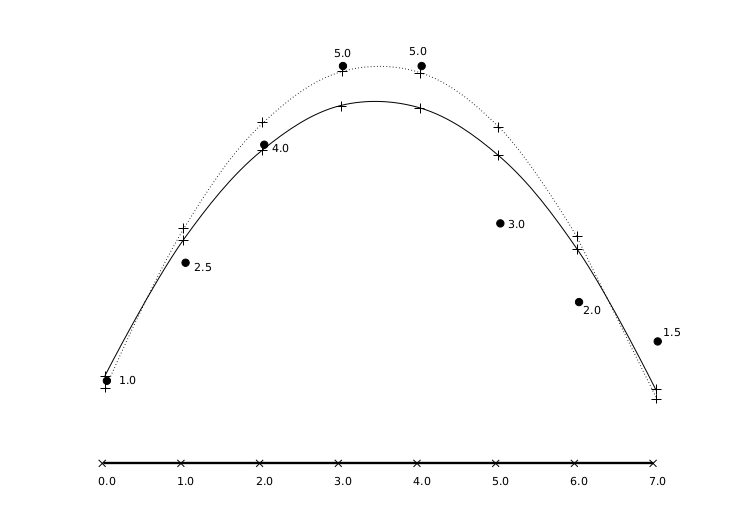
\includegraphics[width=\textwidth]{figures/GLS.png}
	\end{center}
	\caption{Global Least Squares (solid curve) and Weighted Global Least Squares (dashed curve) fit for data represented by the solid circles. The fit is a quadratic fit. The weighting used for the dashed curve is 1.0 every where except at x = 3.0 and x = 4.0 where it is 10.0 (\cite{MLSIntro})}
	\label{fig:gls_example}
\end{figure}
\subsection{Weighted GLS}
We can assign each data value a weight w to use in the least squares fit, so that we write the objective function to be minimized as:
\begin{equation}
	R^{WGLS} = \sum_i{w_i \cdot (u_i - u(x_i)^2} = \sum_i{w_i \cdot (u_i - \sum_j{b_j(x_i)\cdot c_j})^2}
\end{equation}
The gradient $\nabla_c R^{WGLS}$ is expanded to a linear system:
\begin{equation}
	B^TWBc = B^TWu
\end{equation}
where $W = 
\begin{pmatrix}
	w_1 & 0 	& ... & 0\\
	0 	& w_2 	& ... & 0\\
	...\\
	0 	& 0 	& ... & w_n\\
\end{pmatrix}$ is a diagonal matrix with $W_{i,i} = w_i$. Figure \ref{fig:gls_example} shows an example of a weighted global least squares approximation.\\
The solution is obtained by solvong $c = (B^TWB)^{-1}\cdot B^TWu$
\subsection{Weighted Local Least Squares}
In global least squares fitting, we assumed that the function represented by the data can be accurately captured by a single polynomial spanning the entire domain. For large, complex data sets, however, this would require to fit a polynomial of an impractically high order and even then it may not capture all the features of the data. So instead of a global solution, the better picture of the solution can be obtained by fitting lower order polynomials to each data point $(x_p, u_p)$ and its neighbors. Thus there are N least squares fits $u_i(x)$ , each one approximating the solution at point $x_i$ and the coefficient vector $c_i$ is different at each point. Note that this is not a well-established method and is not in common use, however, it is perfectly aligns with the correction of SDF grid, which is generated by the fluid reconstruction methods.\\
The approximate solution for point $x_p$ is evaluated through $R^{WLLS}_p = \sum_i^N w_{pi} \cdot (u_i - u(x_i))^2$, where $i\in [1, N]$ are neighbors of $x_p$. The gradient is expanded to matrix equation: $B^T W_p Bc_p = B_p^T W_p u$.\\
Unlike the Weighted Global Least Squares fit, there isn’t necessarily only one approximate solution at any point x in the domain since the neighborhoods of the local solutions overlap. Then the first choice we have for evaluating $u(x)$ is to use the local solution $u_p(x)$ at the point $x_p$. The other method could be averaging all solutions, which were calculated for point $x_p$ within its neighbors:
\begin{equation}
	u(x) = \dfrac{1}{n} \sum_{i=1}^n{u_i(x)}
\end{equation}
An example of what quadratic functions fitted to each point and its neighbors might look like is shown in Figure \ref{fig:WLLS}
\begin{figure}[H]
	\begin{center}
		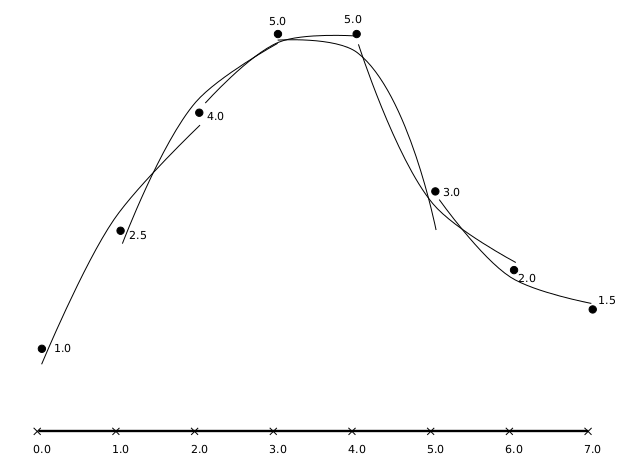
\includegraphics[width=\textwidth]{figures/WLLS.png}
	\end{center}
	\caption{Weighted Local Least Squares fit for given data. Note the overlapping approximations at most points (\cite{MLSIntro})}
	\label{fig:WLLS}
\end{figure}

More discussion on the MLS for arbitrary point in space and Local Regression estimator could be found in \cite{MLSIntro}. In this thesis WLLS approach will be used to correct SDF of the MC grid domain.

\section{Algorithm}
In the Algorithm \ref{alg:mls_alg} general overview of the mls smoothing filter on MC SDF grid is described. The filter can be applied iteratively, similarly to blur filter.
\begin{algorithm}[H]
	\scriptsize
	\begin{algorithmic}
		\State generate set of 0-level intersection vertices 
		\State generate neighborClusters form 0-level intersection vertices 
			
		\ForAll{$cluster \in neighborClusters$}
			\State find mls surface approximation for cluster (surfApproximation)
			\ForAll{$vertex \in cluster$}
				\State $newSDF[vertex] \gets newSDF[vertex] + computeUpdatedSDF(vertex, surfApproximation)$
				\State $weights[vertex] \gets weights[vertex] + 1$
			\EndFor
		\EndFor

		\ForAll{$\{vertex, weight\} \in weights$}
			\State $sdfFactor \gets min\left(1, smoothingFactor \cdot \dfrac{fluidParticles[vertex]}{maxFluidParticles}\right)^2$
			\State $newSDF[vertex] \gets sdfFactor \cdot \dfrac{newSDF[vertex]}{weight} + oldSDF[vertex] \cdot (1 - sdfFactor)$
		\EndFor
		\State return levelSet
	\end{algorithmic}
	\caption{mls smoothing filter algorithm}
	\label{alg:mls_alg}
\end{algorithm}
As an input we have an old SDF, computed by underlying reconstruction method (e.g. Dencity based reconstruction, Zhu \& Bridson, Solenthaler). The algorithm computes 0-level intersection vertices - vertices from which final surface mesh will be extracted by linearly interpolating the SDF's between two neighboring vertices with different SDF signs. This is required as soon as the MLS by definition reconstructs surfaces from SDF that represents a distance to a surface (e.g. tuple $(x_p, u_p)$ is a position in space and distance to the surface). However, in the underlying reconstruction methods computed SDF does not represents the distance to a surface along the whole domain of MC grid. Only the SDF values of 0-level intersection vertices are assumed to be a a distances to a surface, thus can be used for mls approximation. Intersection cells are shown in the Figure \ref{fig:intersection_vertices}.\\
\begin{figure}[H]
	\begin{center}
		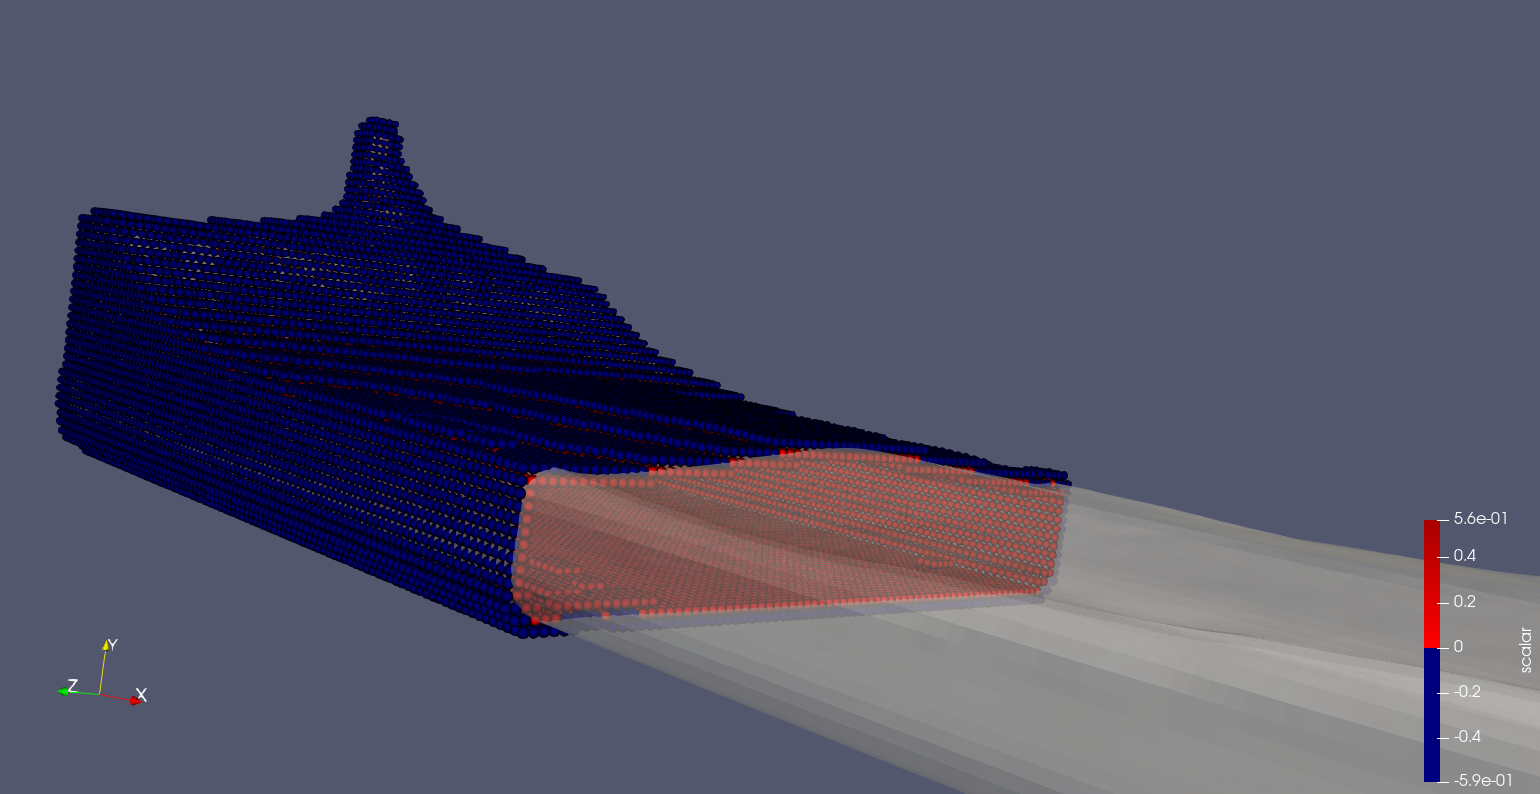
\includegraphics[width=\textwidth]{figures/MlsIntersectionVertexSet.png}
	\end{center}
	\caption{0-level intersection MC grid vertices. Red are vertices with positive SDF sign, blue are one with negative sign}
	\label{fig:intersection_vertices}
\end{figure}

Another advantage of using set of 0-level intersection vertices for mls approximation is that the algorithm can exactly determine the set of neighbor MC vertices that lie along the reconstructed surface, without approximating the surface normal and taking approximate neighbor set along the tangential direction to the normal. Some computed clusters are represented in the Figure \ref{fig:clusters}\\
\begin{figure}[H]
	\begin{center}
		\begin{subfigure}[b]{0.45\textwidth}
			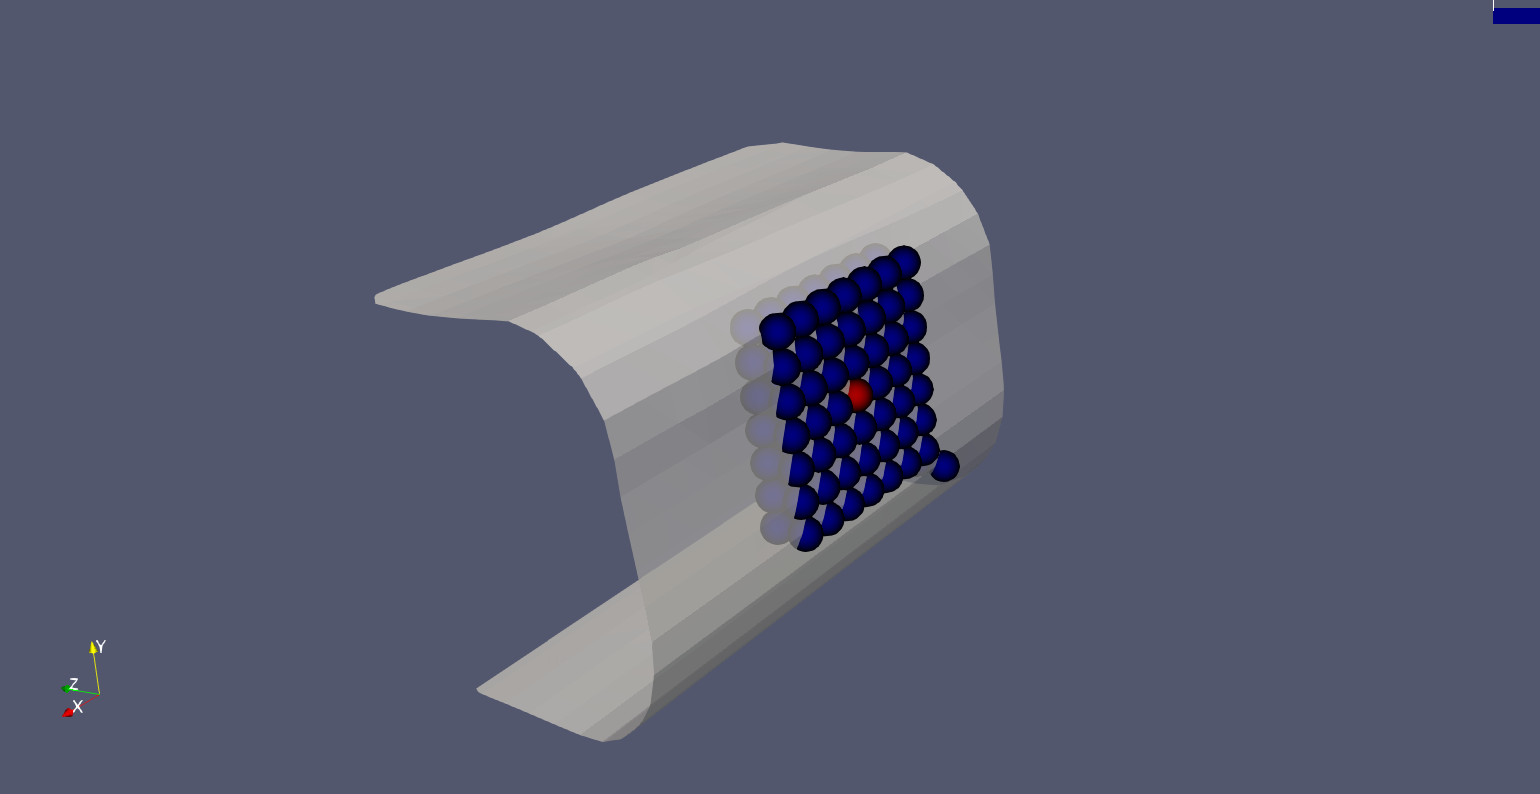
\includegraphics[width=\textwidth]{figures/MlsCluster.png}
		\end{subfigure}
		\begin{subfigure}[b]{0.45\textwidth}
			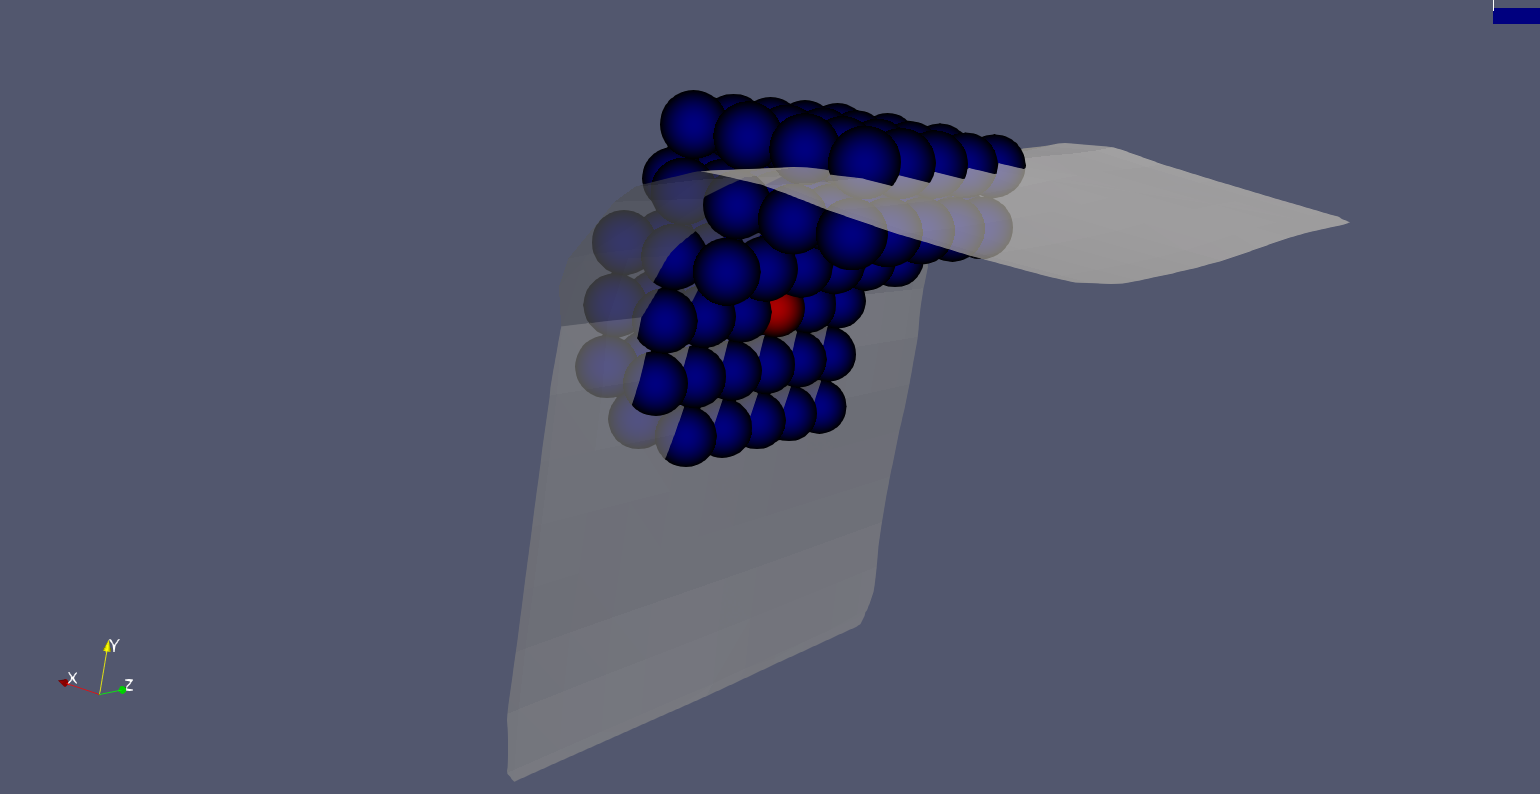
\includegraphics[width=\textwidth]{figures/MlsCluster2.png}
		\end{subfigure}
	\end{center}
	\caption{Examples of computed clusters. Red sphere is a reference vertex w.r.t. which cluster is computed.}
	\label{fig:clusters}
\end{figure}

And the last important advantage is a performance optimization, as far as there is no need to compute costly mls approximation for each MC grid vertices in the domain.\\

However, there is no guarantee that after the applying approximation the SDF sign of the MC grid vertex will not be switched, e.g. if some MC grid vertex had a positive SDF value before smoothing, after mls approximation it can take a negative value. In this case the set of 0-level intersection vertices set will be changed, and some of the MC grid vertices, that was not mls smoothed will be used during the final surface generation and can bring unnecessary noise to the reconstructed surface. This issue can be worked around by applying multiple iteration of mls smoothing trading off final surface smoothness and reconstruction performance.\\

The set of 0-level intersection vertices is split into clusters. For each cluster coefficients of mls approximated surface is computed using WLLS approach, and based on the obtained solution new SDF values are generated for each vertex in the cluster. As soon as vertices can appear in multiple clusters the total values are summed up and then the final value should be divide by a sum of weights applied for mls values. For simplicity and maximization of surface smoothing it was decided set final mls corrected SDF to a average of the mls approximations computed for point vertex $x_p$ is each cluster e.g.:
\begin{equation}
	SDF(x_p) = \dfrac{1}{N} \sum_{i = 0}^N{SDF_{C_i}(x_p)}
\end{equation}
where $C_i$ are all clusters such, that $x_p \in C_i$.\\

For thin and small feature areas, where smoothing could destroy small features or even introduce artifacts, smoothing factor is computed and applied to the final mls value as a weighted sum between the old SDF value and new mls corrected SDF value. The smoothing factor is applied similarly to Blur filter.\\

\subsection{Clusters computation}
After computing the 0-level intersection vertices of MC grid, clusters are computed. The clusters are a set of neighbor vertices, picked from the 0-level intersection vertices set, which, after all, will be used to compute a mls approximation. The Algorithm \ref{alg:computeClusters} describes the procedure of clusters generation.
\begin{algorithm}[H]
	\scriptsize
	\begin{algorithmic}
			\State $vertices \gets ZeroLevelIntersectionVertices$
			\While{$vertices$ is not empty}
				\State $vertex \gets vertices.top()$
				\State compute vertex curvature

				\State $maxSamplesFactor \gets \left(\dfrac{min(\dfrac{1}{|curvature|}, FluidParticleDiameter \cdot FluidParticlesForCurvatureRadius)}{FluidParticleDiameter \cdot FluidParticlesForCurvatureRadius}\right)^2$
				\State $samplesCount \gets MlsSamples \cdot maxSamplesFactor$

				\State $cluster \gets getNeighbourCells(ZeroLevelIntersectionVertices, vertex, samplesCount)$
				\State add cluster to clusters
			\EndWhile
			\State return clusters
	\end{algorithmic}
	\caption{mls clusters computation}
	\label{alg:computeClusters}
\end{algorithm}
Here $ZeroLevelIntersectionVertices$ is a previously computed set of MC grid vertices  that are in the neighborhood of the 0-level SDF,  
$FluidParticleDiameter$ is a diameter of a SPH fluid particles, $FluidParticlesForCurvatureRadius$ is a number of particles that can fit in a mean curvature radius (more explanations later), $MlsSamples$ - user defined maximum number of neighbor vertices in the cluster.\\
Before the algorithm iterates over the vertices in the 0-level intersection set, they are duplicated in separate storage($vertices$). This is required to be able to remove some of the neighbor vertices from the intersection vertex set to avoid re-computation of the clusters for this vertices. In the mean time unchanged set of $ZeroLevelIntersectionVertices$ is to be used in the neighborhood search algorithm for clusters. This step adds a trade-off between the reconstruction runtime and surface quality. More explanations will be added in next sections.\\
Next the curvature of the current processed vertex is computed. To save a sharp features of the fluid surface it was decided to decrease the number of neighbors in the cluster, for which mls approximation will be applied. Based on the mean curvature of current 0-level intersection vertex number of samples in the cluster is computed, which is a fraction [1, MlsSamples]. The curvature is computed using the method described in \cite{CurvatureComputation}. firstly compute the curvature for each surface particle that resides in
this cell with the help of its neighboring particles as:
\begin{equation}
	c_i = \sum_j{(1 - n_i \cdot n_j)\cdot k_c(x_i-x_j, h)}
\end{equation}
where $j$ stands for the neighboring particles, $n_i, n_j$ are SPH particle normals and
$k_c$ is the kernel function defined as:
\begin{equation}
	k_c(x_i-x_j, h) = max\left(0, \dfrac{1 - |x_i - x_j|}{h}\right)
\end{equation}
Finally, the curvature of any surface cell is approximated as:
\begin{equation}
	c_{cell} = \dfrac{\sum_i{c_i}}{N}
\end{equation}
where i and N represent the surface particles and the total number of surface particles inside the cell, respectively. The factor $maxSamplesFactor$ reaches valuation of 1 for all vertices, for which mean curvature radius exceeds value of $FluidParticleDiameter \cdot FluidParticlesForCurvatureRadius$. Optimal solution for this thesis was to use $FluidParticlesForCurvatureRadius=50$

\subsection{MLS neighborhood search}
Neighbors detection is described in pseudo-code of Algorithm \ref{alg:mls_nbsearch}
\begin{algorithm}[H]
	\scriptsize
	\begin{algorithmic}
		\State push $BaseMcVertex$ to $todoMlsVertices$
		\While{$sizeof(neighborCells) < MlsSamples \land todoMlsVertices \ne \emptyset$}
			\State $currentMcVertex \gets todoMlsVertices[0]$
			\State $todoMlsVertices \gets todoMlsVertices \ todoMlsVertices[0]$
			\If{$indexOf(currentMcVertex) \in SelectedIndices \lor SelectedIndices = \emptyset$}
				\State push currentMcVertex back to neighborCells
			\EndIf
			\ForAll{ $nc \in nearest neighbors of currentMcVertex$}
				\If{$nc \in ZeroLevelIntersectionVertices \land nc \not\in neighborCells \land nc \not\in todoMlsVertices$}
					\State push $nc$ back to todoMlsVertices;
				\EndIf
			\EndFor
		\EndWhile
		return neighborCells;
	\end{algorithmic}
	\caption{mls MC vertex neighbors search}
	\label{alg:mls_nbsearch}
\end{algorithm}
As an input procedure receives a $BaseMcVertex$ - a MC vertex for which neighborhood cluster is going to be computed, $ZeroLevelIntersectionVertices$ - 0-level intersection MC vertices explained previously, and $SelectedIndices$ - a set of indexes of neighbors, that should be accepted as a samples (more explanations are in the next section). The procedure returns a set of MC grid vertices, that are in the nearest neighborhood within a requested $BaseMcVertex$, and which are in a set of 0-level intersection MC vertices. The computed array has some important properties, that will be exploited further. First of all, the further the neighbor is from the base cell the higher index it has inside the array. Figure \ref{fig:mls_neighbor_alignment} shows the example of alignment of detected cluster neighbors in the set of 0-level intersection vertices.\\
\begin{figure}[H]
	\begin{center}
		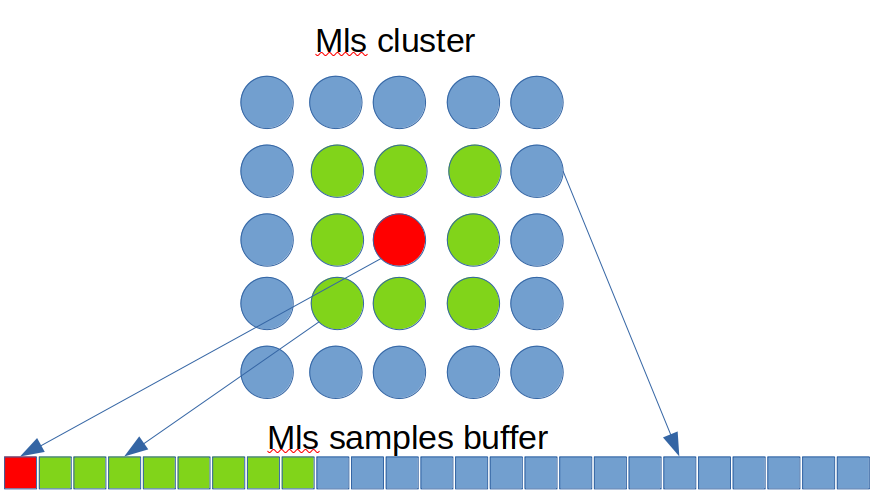
\includegraphics[width=\textwidth]{figures/MlsSamplesBufferAlignment.png}
	\end{center}
	\caption{Mapping of mls samples from cluster to buffer (2d slice view)} \label{fig:mls_neighbor_alignment}
\end{figure}
\subsubsection{MlsSamples}
The final neighborhood is formed as an area of MC vertices along the 0-level iso surface. The larger MlsSamples the wider area of samples within the requested base sample will be computed and the more smoothing will be applied to the SDF, e.g. some examples of computed neighborhood area depending on a number of MlsSamples and respective reconstructed surface are shown in the figure \ref{fig:mls_samples_example_surfaces}.
\begin{figure}[H]
	\begin{center}
		\begin{subfigure}[b]{0.49\textwidth}
			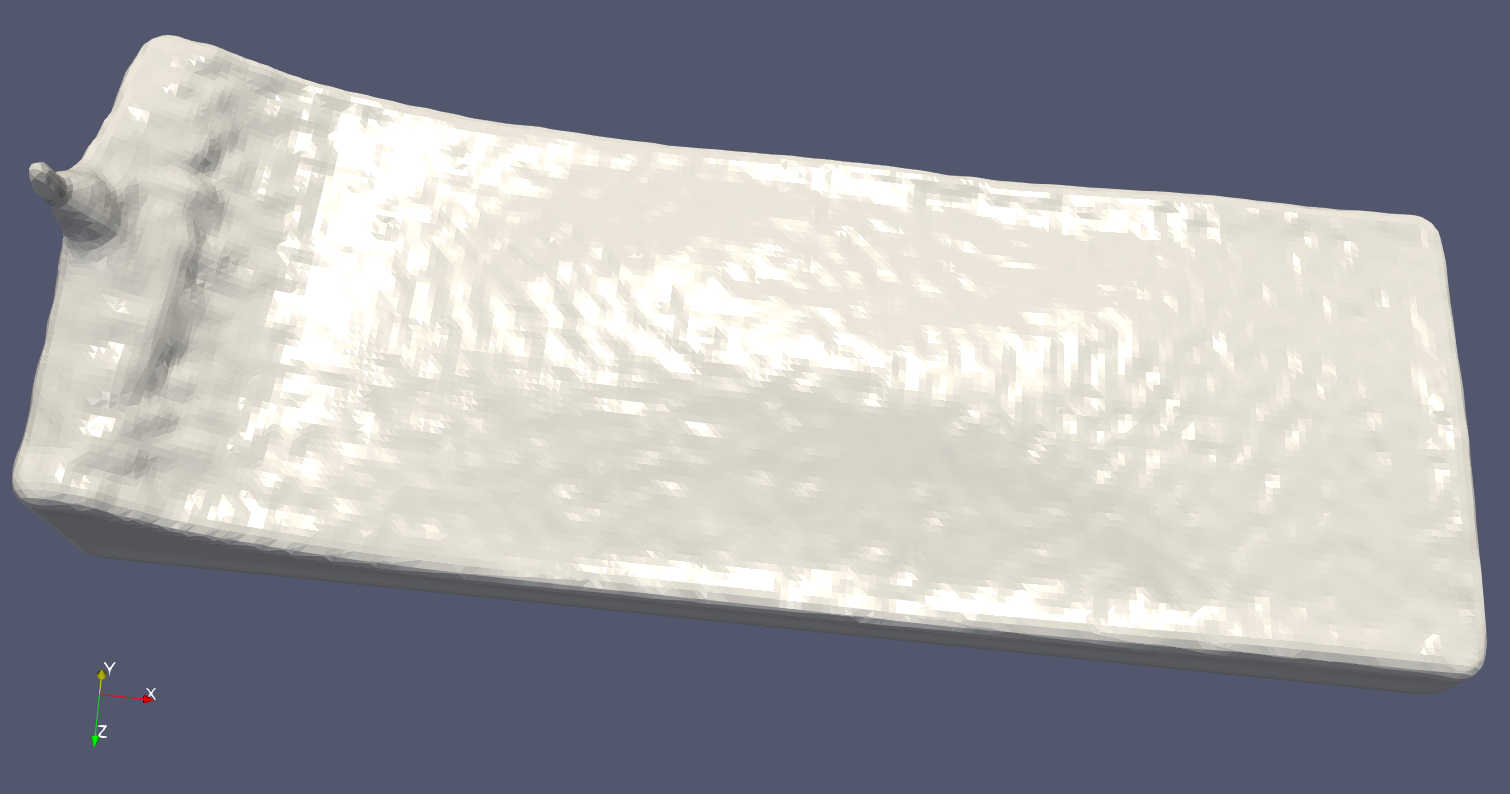
\includegraphics[width=\textwidth]{figures/MlsSamples10.png}
			\caption{10 samples}
		\end{subfigure}
		\begin{subfigure}[b]{0.49\textwidth}
			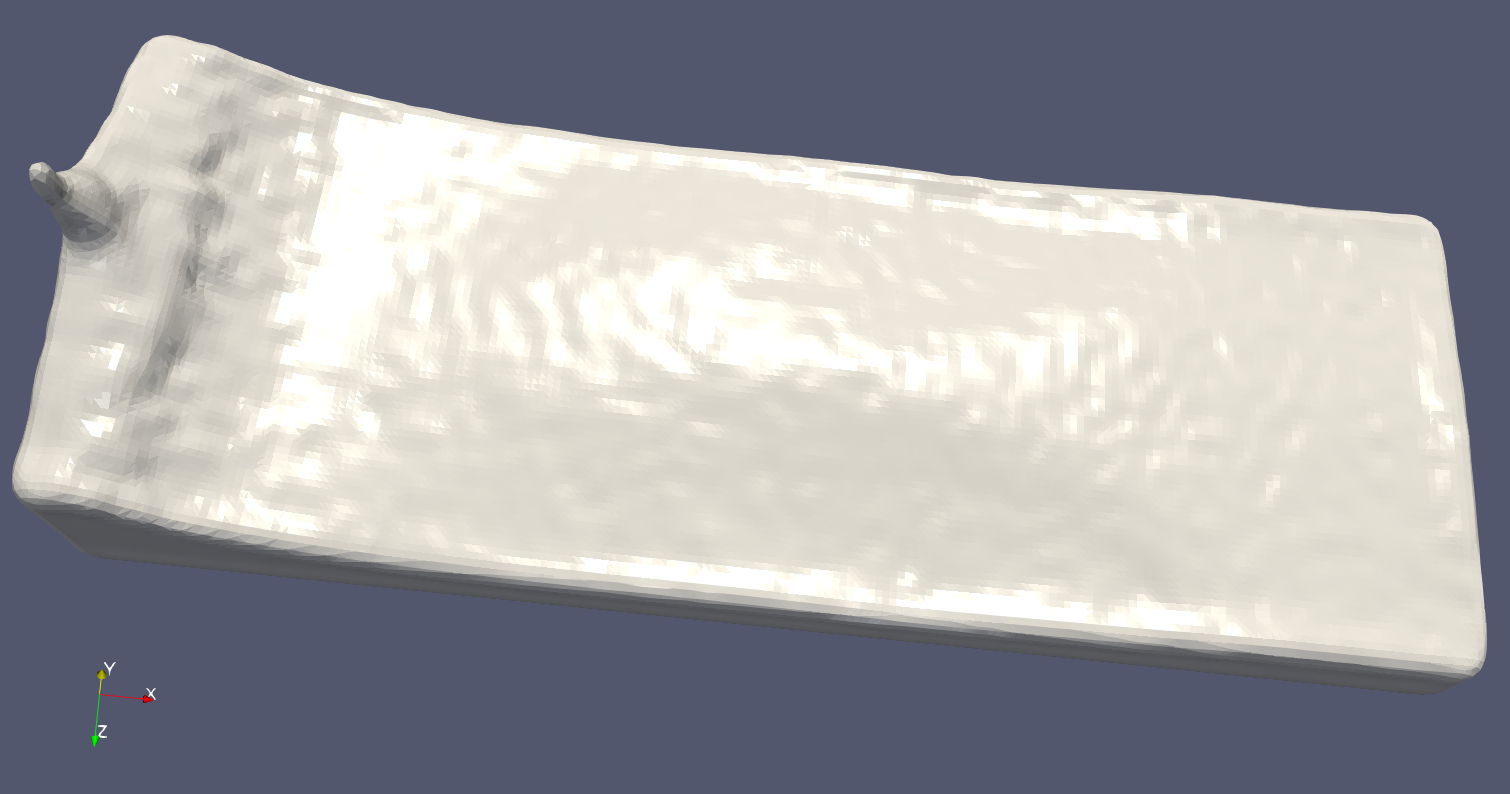
\includegraphics[width=\textwidth]{figures/MlsSamples40.png}
			\caption{40 samples}
		\end{subfigure}
		\begin{subfigure}[b]{0.49\textwidth}
			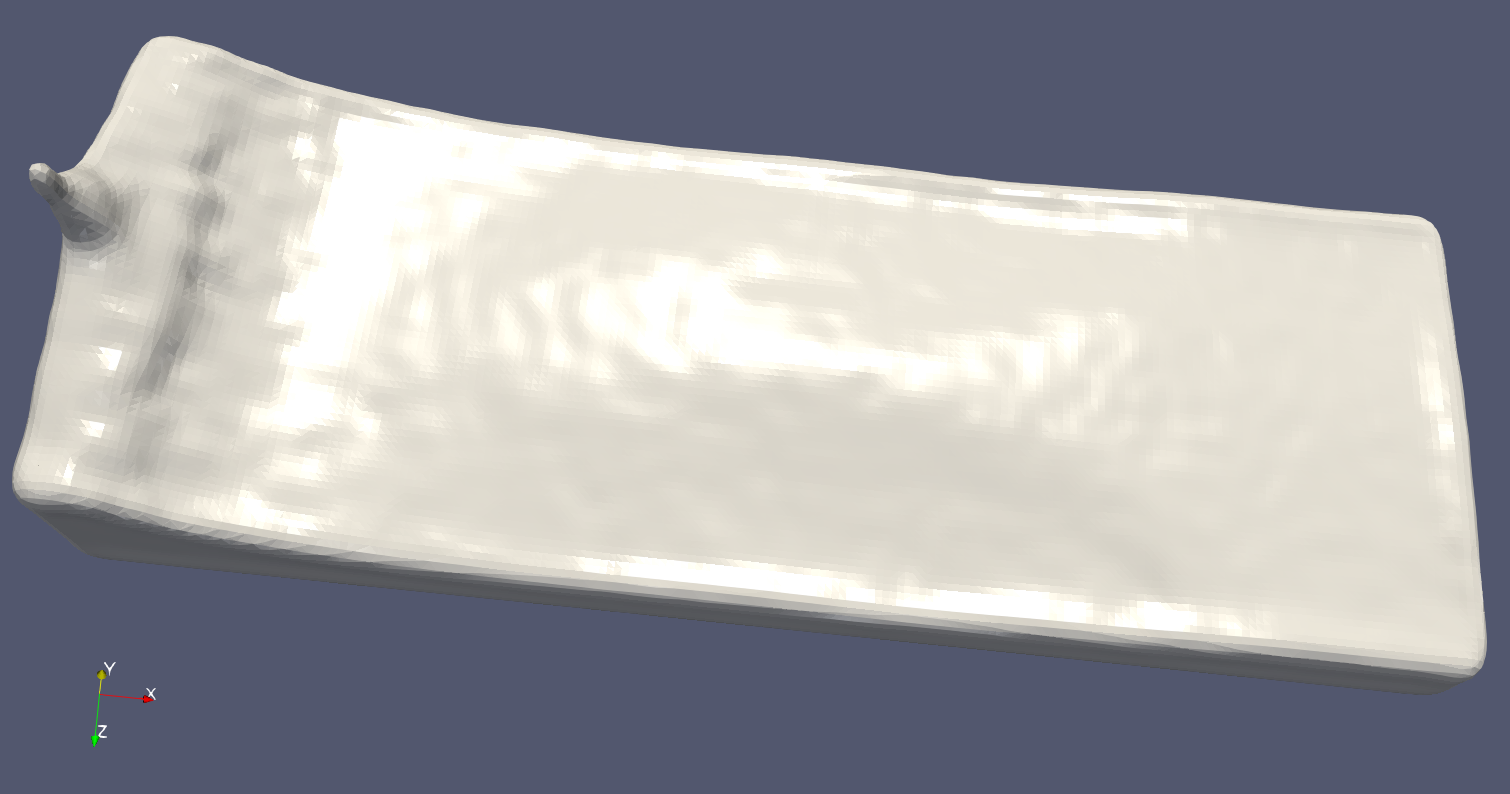
\includegraphics[width=\textwidth]{figures/MlsSamples80png.png}
			\caption{80 samples}
		\end{subfigure}
		\begin{subfigure}[b]{0.49\textwidth}
			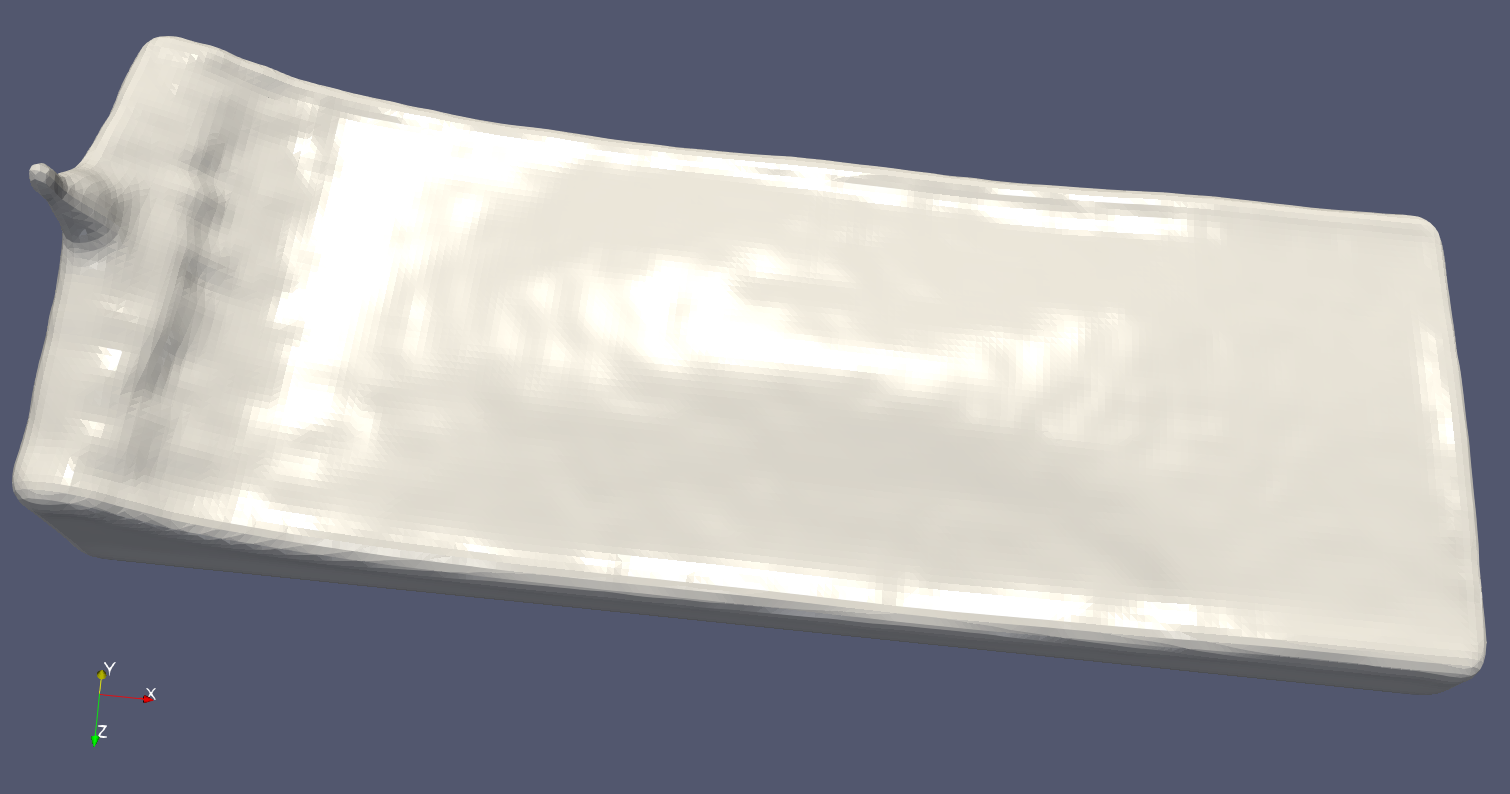
\includegraphics[width=\textwidth]{figures/MlsSamples100.png}
			\caption{100 samples}
		\end{subfigure}
	\end{center}
	\caption{Surface quality depending on the number of mls samples} \label{fig:mls_samples_example_surfaces}
\end{figure}
Thus modifying number of mls samples influences the final surface quality as well as reconstruction time. In general complexity of the mls smoothing can be estimated as $O(n \cdot m)$, where $m$ is a number of mls samples and $n$ is number of 0-level intersection vertices.
\subsubsection{SelectedIndices}
To receive a smooth surface it is required to use a large amount of mls samples in the neighborhood as was already shown in previous section. Thus it requires a lot of computational efforts, to generate approximated mls surface and to correct SDF of 0-level vertices. Thus to reduce reconstruction time it was decided to apply Monte Carlo approach to pick a representative subset of samples from the neighborhood cluster, which uniformly represents initially computed set. The hope is that we will be able to correctly detect a distribution so that the final surface quality will not be degraded too much and the computation time of the reconstruction phase will be reduced.\\
The first idea that comes to mind is just uniformly pick $n$ samples from the computed mls sample buffer. But for our needs it is more appropriate to pick samples uniformly from each distance level from the reference sample (central one). Figure \ref{fig:samples_distribution} shows the example of the uniformly distributed samples over distance levels.
\begin{figure}[H]
	\begin{center}
		\begin{subfigure}[b]{0.48\textwidth}
			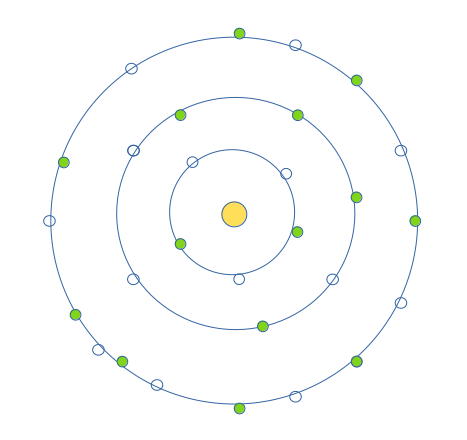
\includegraphics[width=\textwidth]{figures/SampleDistrUnifOverDomain.png}
			\caption{Samples uniformly picked w.r.t. the samples domain}
		\end{subfigure}
		\begin{subfigure}[b]{0.48\textwidth}
			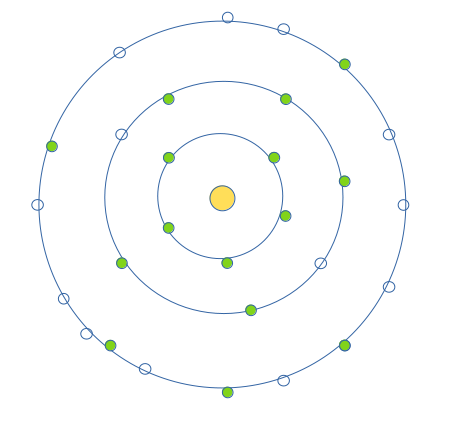
\includegraphics[width=\textwidth]{figures/SampleDistrOverLeveDist.png}
			\caption{Samples uniformly picked from w.r.t. the distance level}
		\end{subfigure}

	\end{center}
	\caption{Example of uniform sampling over points domain and over distance levels}
	\label{fig:samples_distribution}
\end{figure}

The probability of picking samples far away from the base sample is larger then the probability of picking the samples near the base cell, e.g. (for simplicity circle will be used to show  the probability distribution) the density  function of picking arbitrary point, that lies in radius $r$ from the current point is shown in equation \ref{eq:probability_distr}.
\begin{equation}
	p(r) = \dfrac{2 \cdot \pi r}{\pi \cdot R^2} = \dfrac{2 \cdot r}{\cdot R^2}
	\label{eq:probability_distr}
\end{equation}
where $R$ is a radius to the sphere (distance to the outer distance level from reference point). In another words talking the probability of picking sample on that lies from the central sample in a distance of $r$ is equal to length of the inner circle with radius $r$ divided by the area of the sphere.
Thus to pick samples from the buffer uniformly w.r.t. the distance level from the central sample we have to modify the probability distribution of picking a samples from buffer. Next procedure is applied to pick the sample indexes from the buffer uniformly w.r.t. the distance level:
\begin{algorithm}[H]
	\scriptsize
	\begin{algorithmic}
			\State $acceptedIndices \gets \{0\}$;
			\State $lowerBound \gets 0$
			\State $upperBound \gets (MlsSamples - 1)$
			\For{$i \in [0, MaxSamples]$}
				\State $offset \gets \dfrac{PickRandom(0, MaxSamples - 1)}{MaxSamples}$
				\State $index \gets lowerBound + offset^2 \cdot (upperBound - lowerBound))$
				\State $currentIndex \gets index$
				\While{$index \in acceptedIndices$}
					\If{$index = lowerBound$}
						\State $index = upperBound$
					\Else
						\State $index \gets index - 1$
					\EndIf
				\EndWhile
				\State $acceptedIndices \gets acceptedIndices \cup index$;
				\If{$index = lowerBound$}
					\State $index++;$
					\While{$index \in acceptedIndices$}
						\State $index++$
					\EndWhile
					\State $lowerBound \gets index$
				\Else 
					\If{$index = upperBound$}
						\State $index--;$
						\While{$index \in acceptedIndices$}
							\State $index--$
						\EndWhile
						\State $upperBound \gets currentIndex$
					\EndIf
				\EndIf
			\EndFor
	\end{algorithmic}
	\caption{random sampling of indices's in the mls neighborhood}
	\label{alg:mls_montecarlo_sampling}
\end{algorithm}
The idea of the algorithm is to generate set of indexes from domain of mls neighborhood buffer, and after that shift the index to the beginning according to quadratic function $x^2$ where $x\in [0,1]$ is uniformly at random generated position in the array. This way the probability distribution of picking sample from specific distance from the center of the area will be compensated and converge to uniform distribution. Figure \ref{fig:distributions} shows the distributions of sampling indexes before quadratic shifting (uniformly pick the index of the buffer) and after (pick index uniformly and shift it according to the $x^2$ function).\\
\begin{figure}[H]
	\begin{tikzpicture}
		\begin{axis}
			[
				xlabel={$x$},
				ylabel={$y$},
				ymin = 0,
				ymax = 0.1,
				width = 0.45\textwidth
			]
			\addplot[
				red,
				mark=*
			] table{initialDistributionOverLevels.txt};
		\end{axis}

	\end{tikzpicture}
	\begin{tikzpicture}
		\begin{axis}
			[
				xlabel={$x$},
				ylabel={$y$},
				ymin = 0,
				ymax = 0.1,
				width = 0.45\textwidth
			]
			\addplot[
				blue,
				mark=*
			] table{resultingDistributionOverLevels.txt};
		\end{axis}
	\end{tikzpicture}
	\caption{Initial distribution of the samples over area levels (left) and final distribution after modifying indexes (right)}
	\label{fig:distributions}
\end{figure}
where $x$ is a probability of picking sample on distance level $i$ from the center of area, $y$ - is a depth of the distance level. The distributions where generated empirically by sampling 10000 indices's over the whole domain of the buffer. 
\begin{figure}
	\begin{center}
		\begin{subfigure}[b]{0.9\textwidth}
			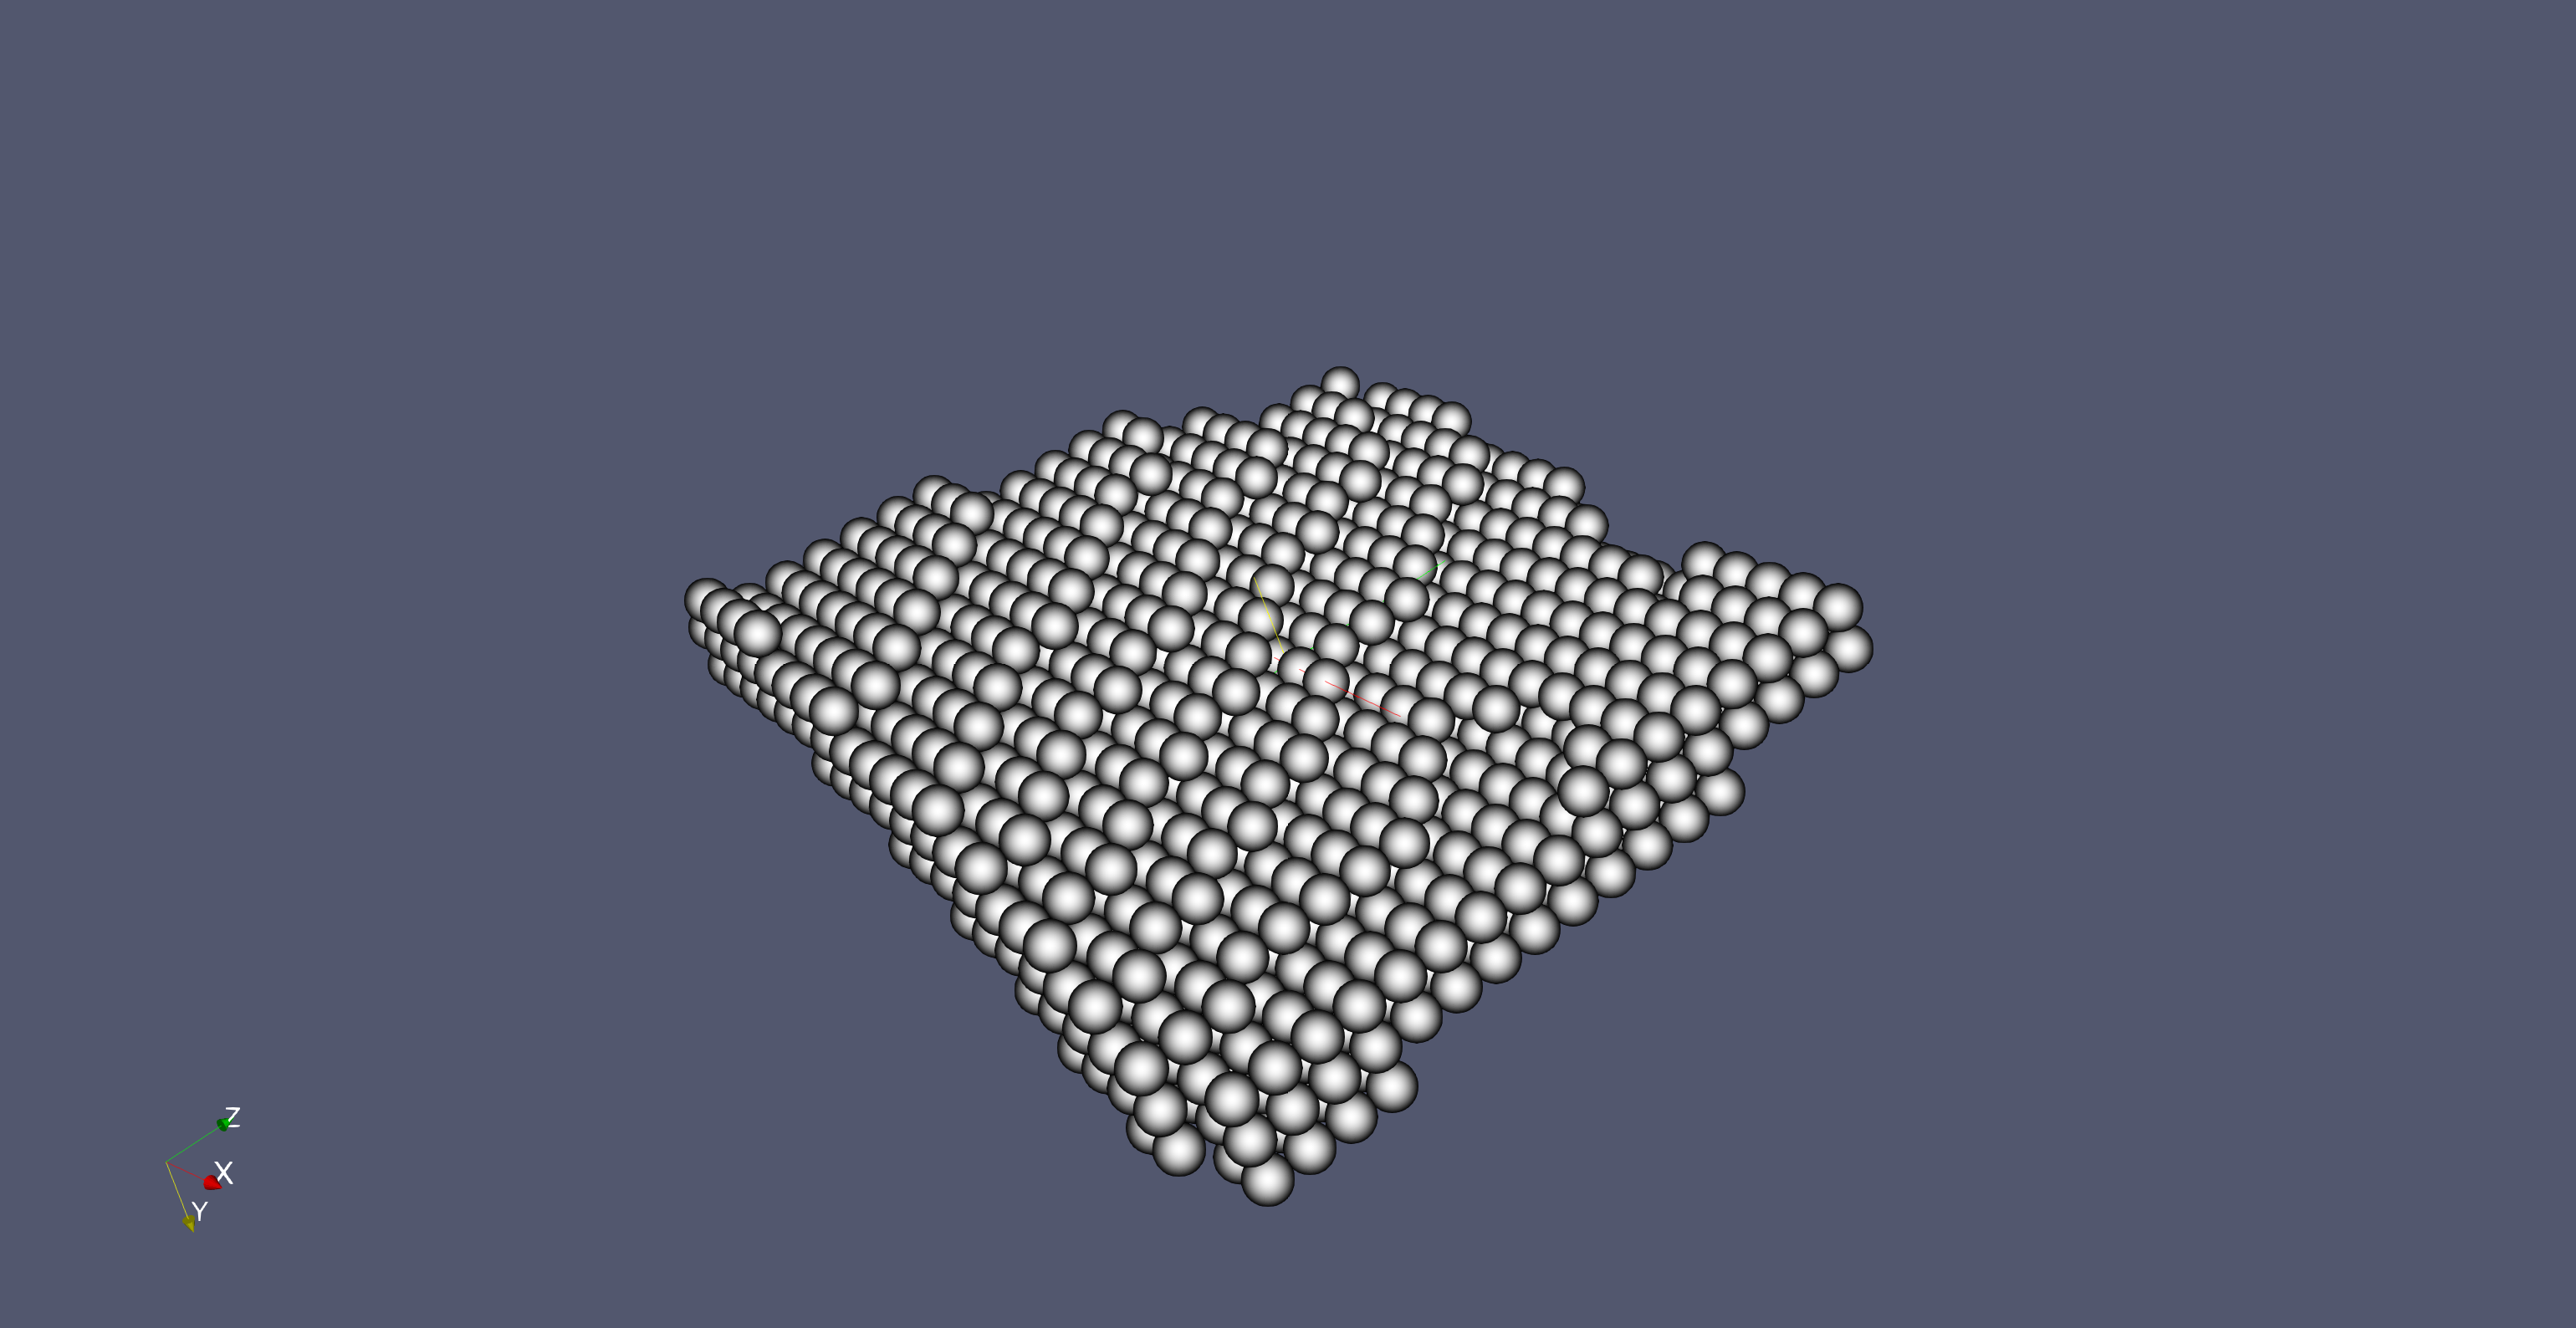
\includegraphics[width=\textwidth]{figures/SamplingFullDomain.png}
			\caption{full set of neighbors}
		\end{subfigure}
		\begin{subfigure}[b]{0.9\textwidth}
			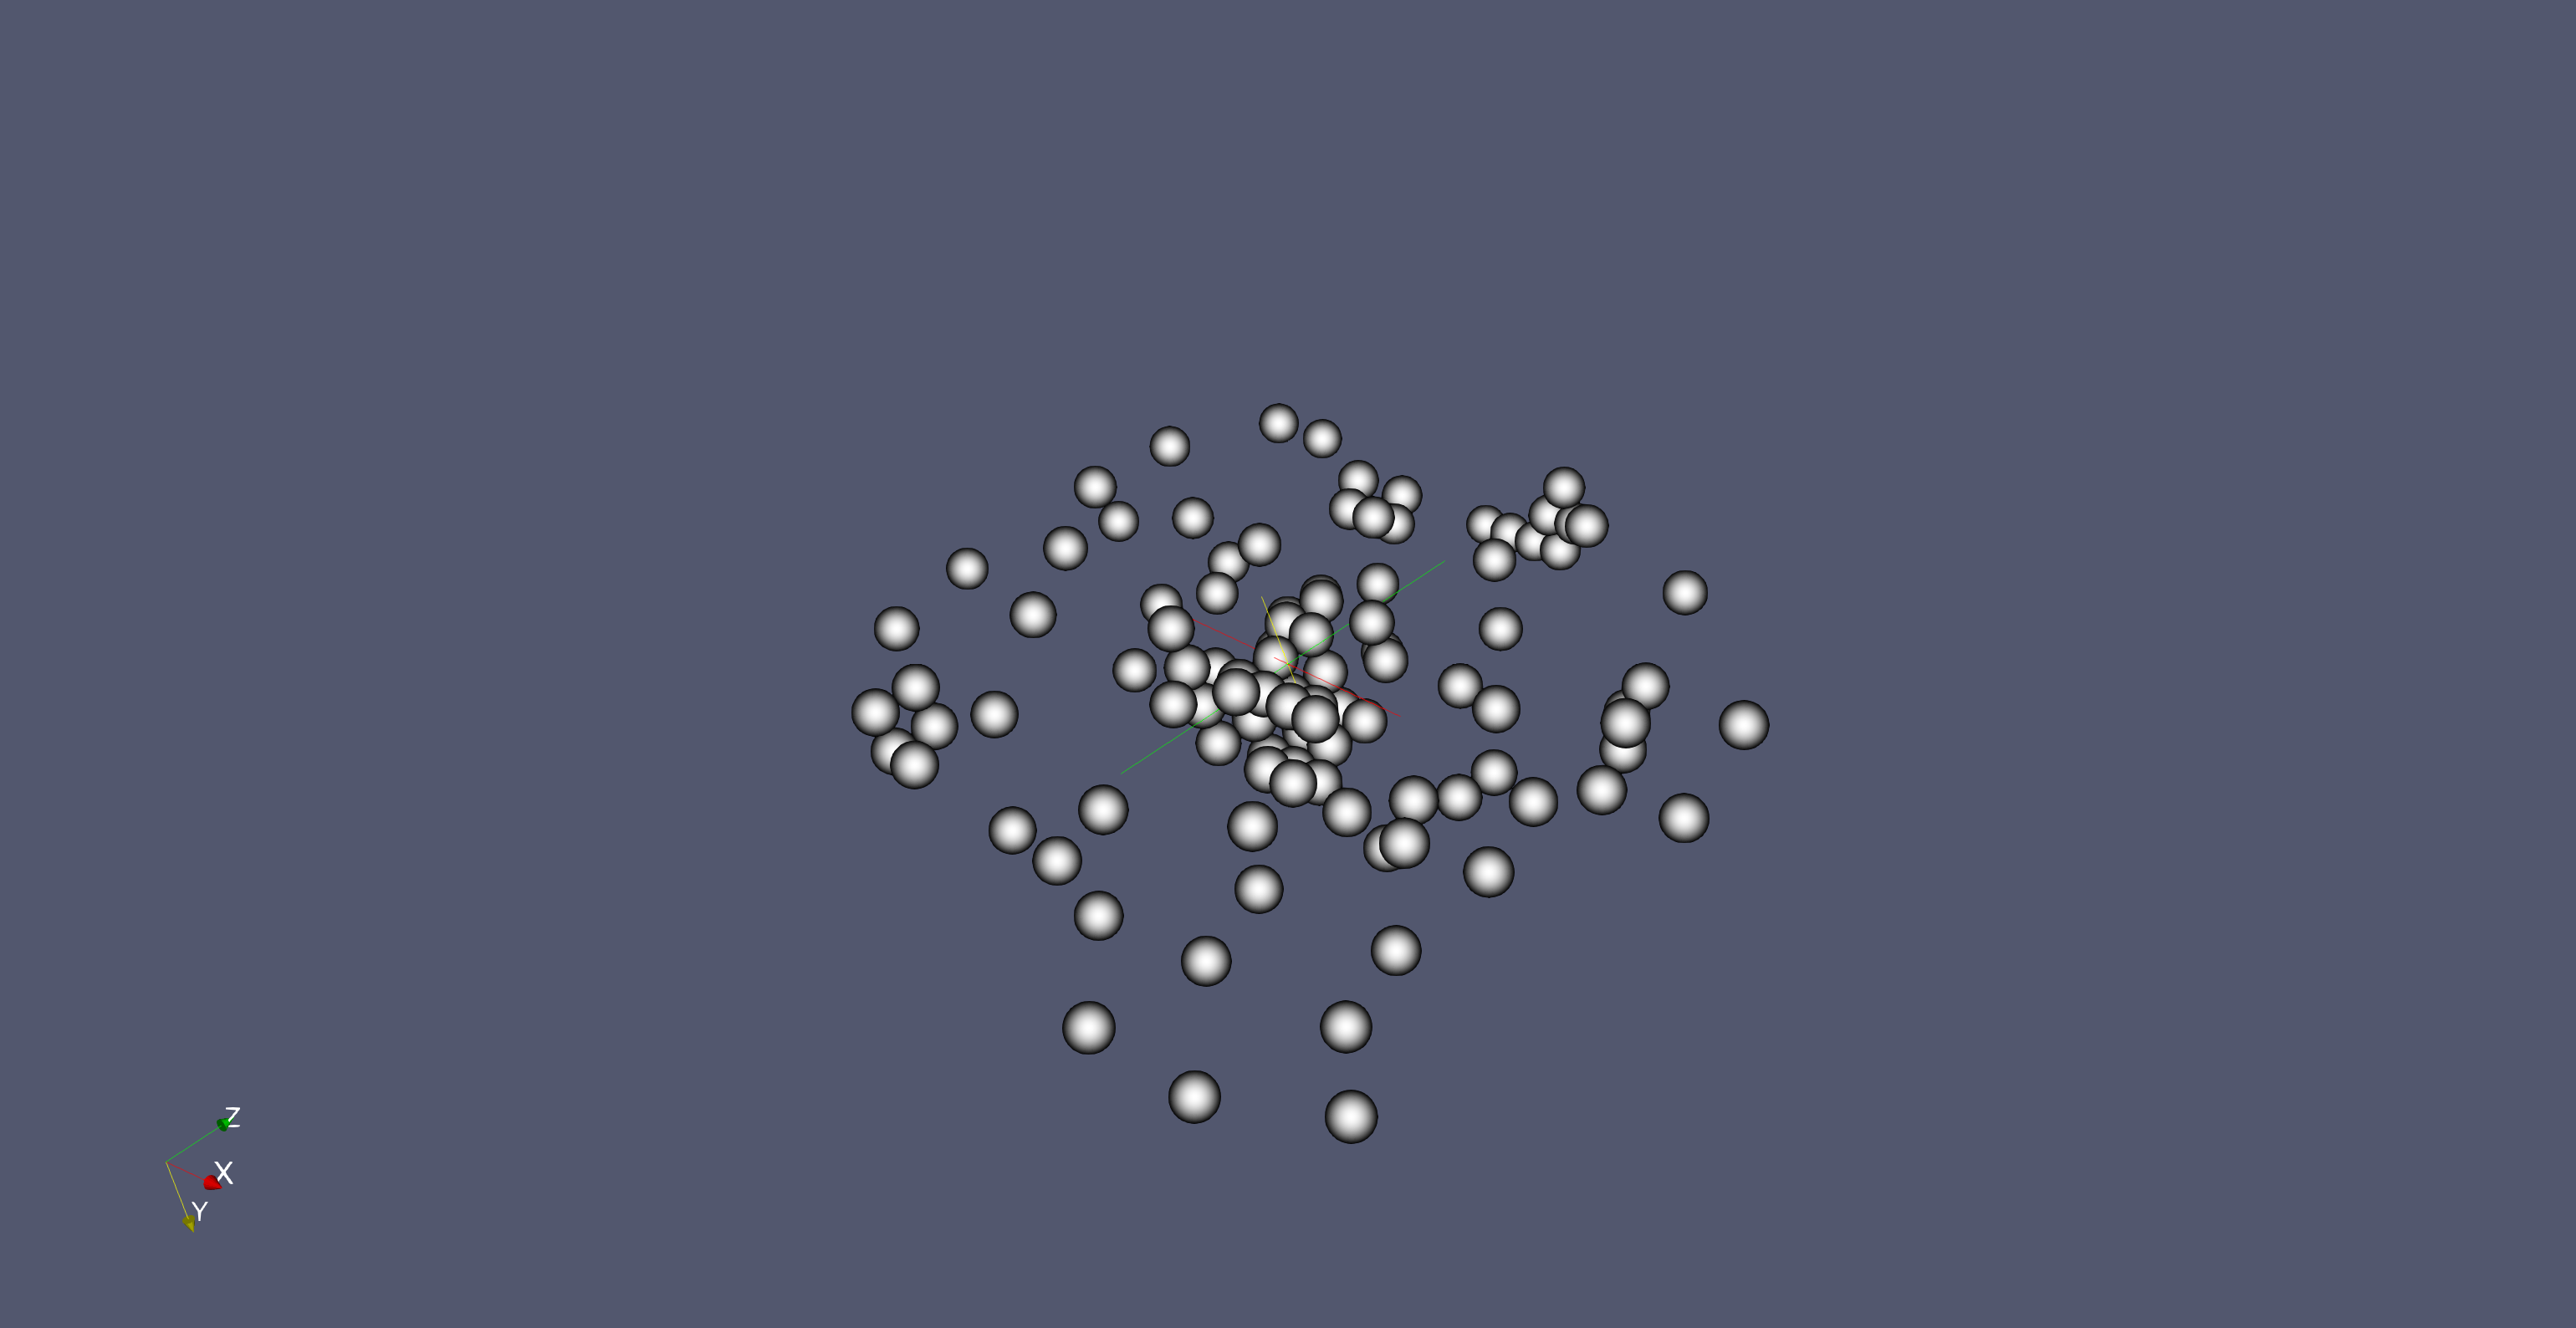
\includegraphics[width=\textwidth]{figures/SamplingQuadratic.png}
			\caption{set of samples with quadratic shift}
		\end{subfigure}
		\begin{subfigure}[b]{0.9\textwidth}
			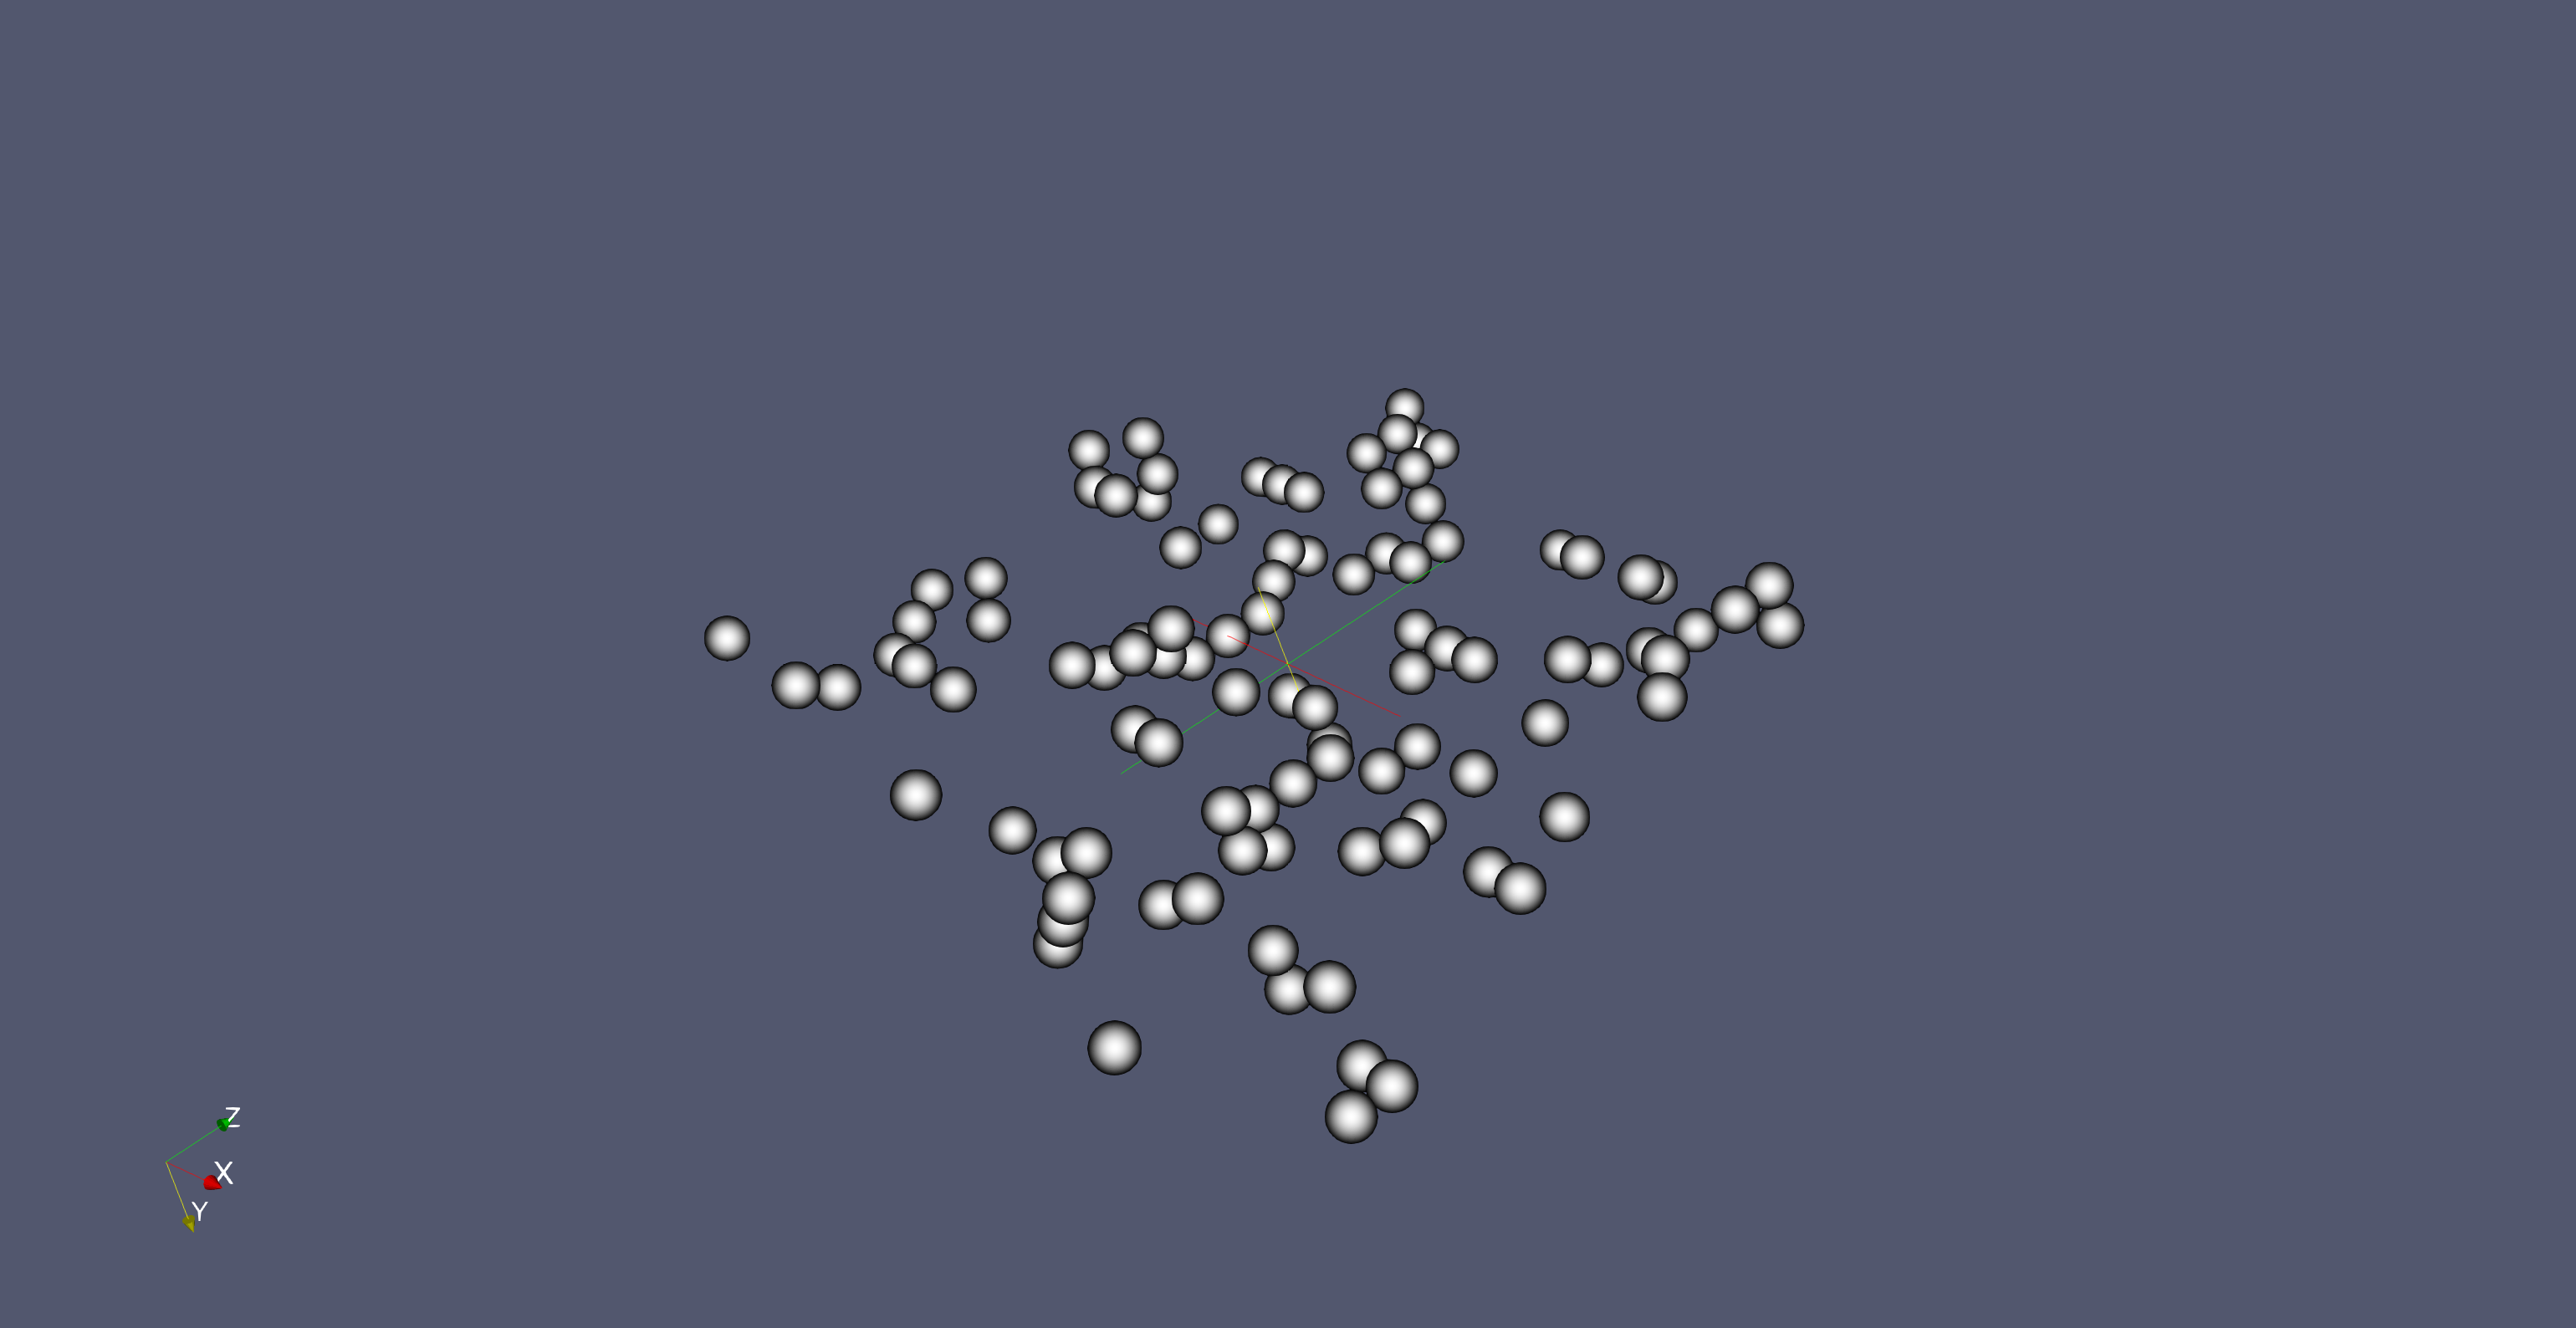
\includegraphics[width=\textwidth]{figures/SamplingUniform.png}
			\caption{uniformly sampled set}
		\end{subfigure}
	\end{center}
	\caption{sampling of mls neighbor vertices set} \label{fig:cluster_sampled}
\end{figure}
In the quadratic shift sampling approach most of the samples are concentrated in the center of the cluster, thus compensating the number of samples, that are far away from the center and that are near to the center. In the uniform approach samples are spreader along the whole area. Figure \ref{fig:cluster_sampled} shows the cluster, with different sampling types.\\
In Figure \ref{fig:surface_sampling_results} some examples of reconstructed scenes using sampled subset of neighbor vertices is shown.
\begin{figure}
	\begin{center}
		\begin{subfigure}[b]{\textwidth}
			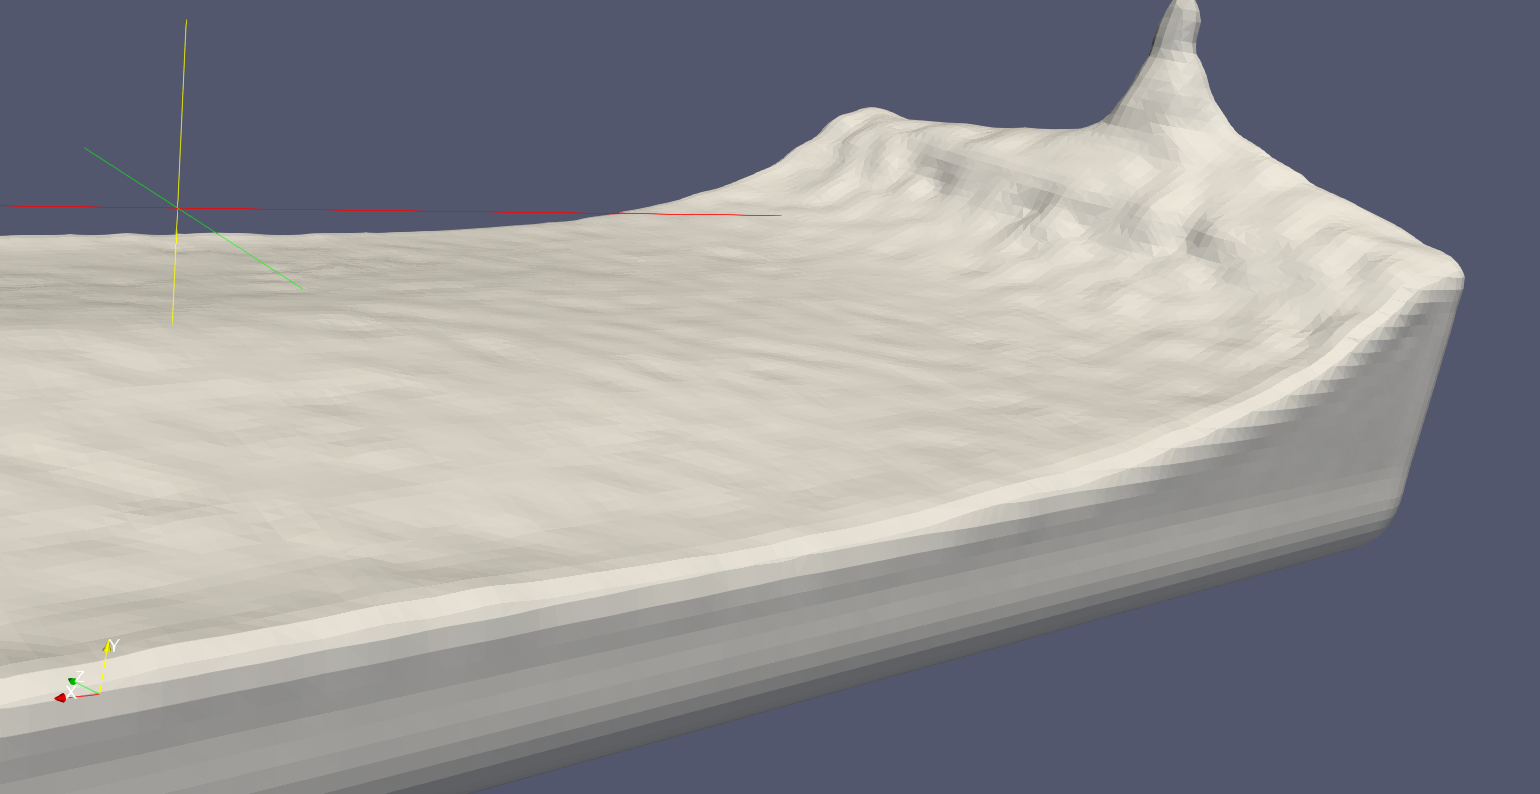
\includegraphics[width=\textwidth]{figures/MLSSurfaceOriginal.png}
			\caption{original surface}
		\end{subfigure}
		\begin{subfigure}[b]{\textwidth}
			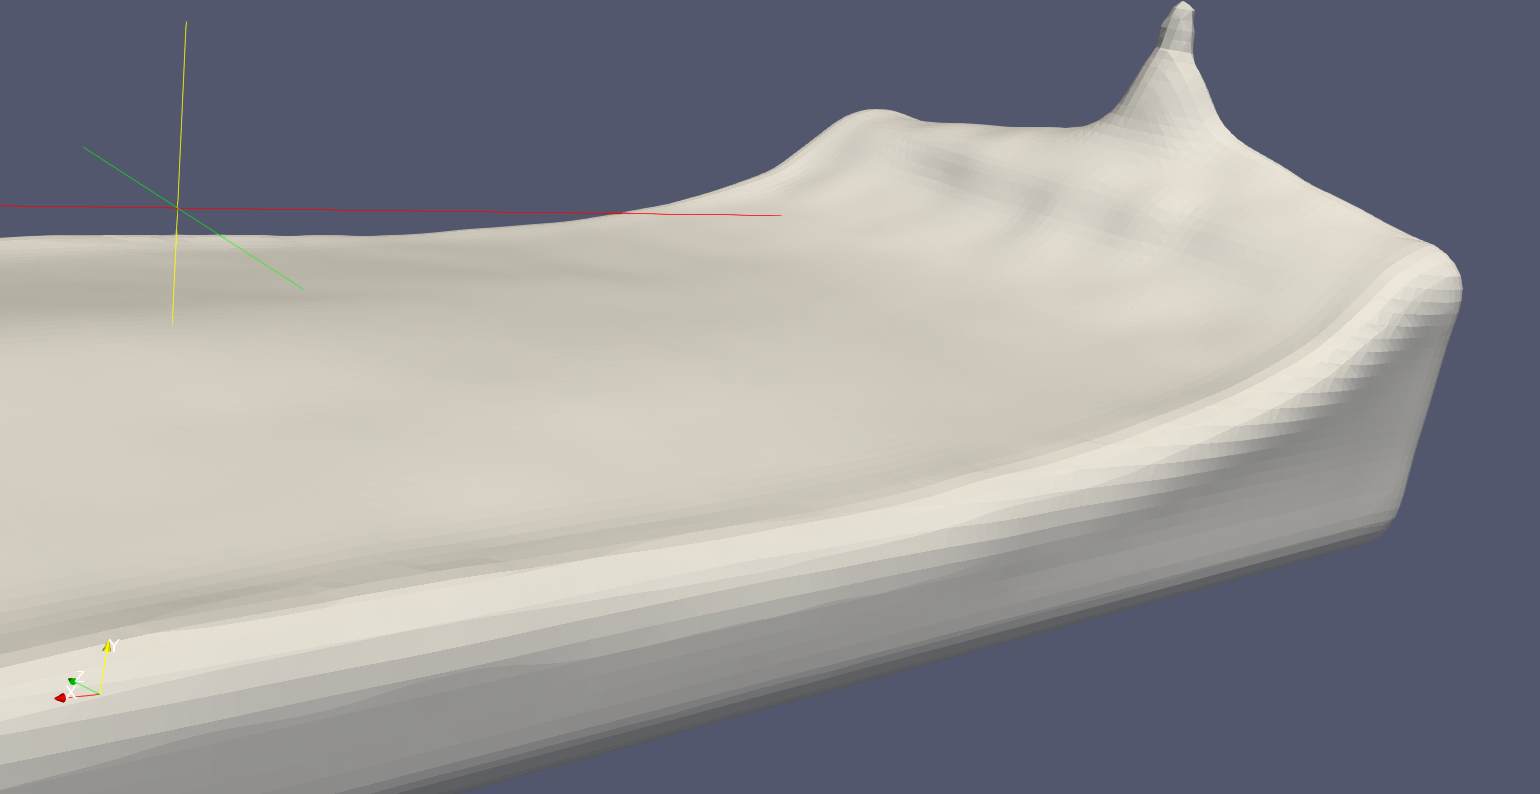
\includegraphics[width=\textwidth]{figures/MLSSurfaceSamplingFullSet.png}
			\caption{mls corrected surface with full set of samples}
		\end{subfigure}
		\begin{subfigure}[b]{\textwidth}
			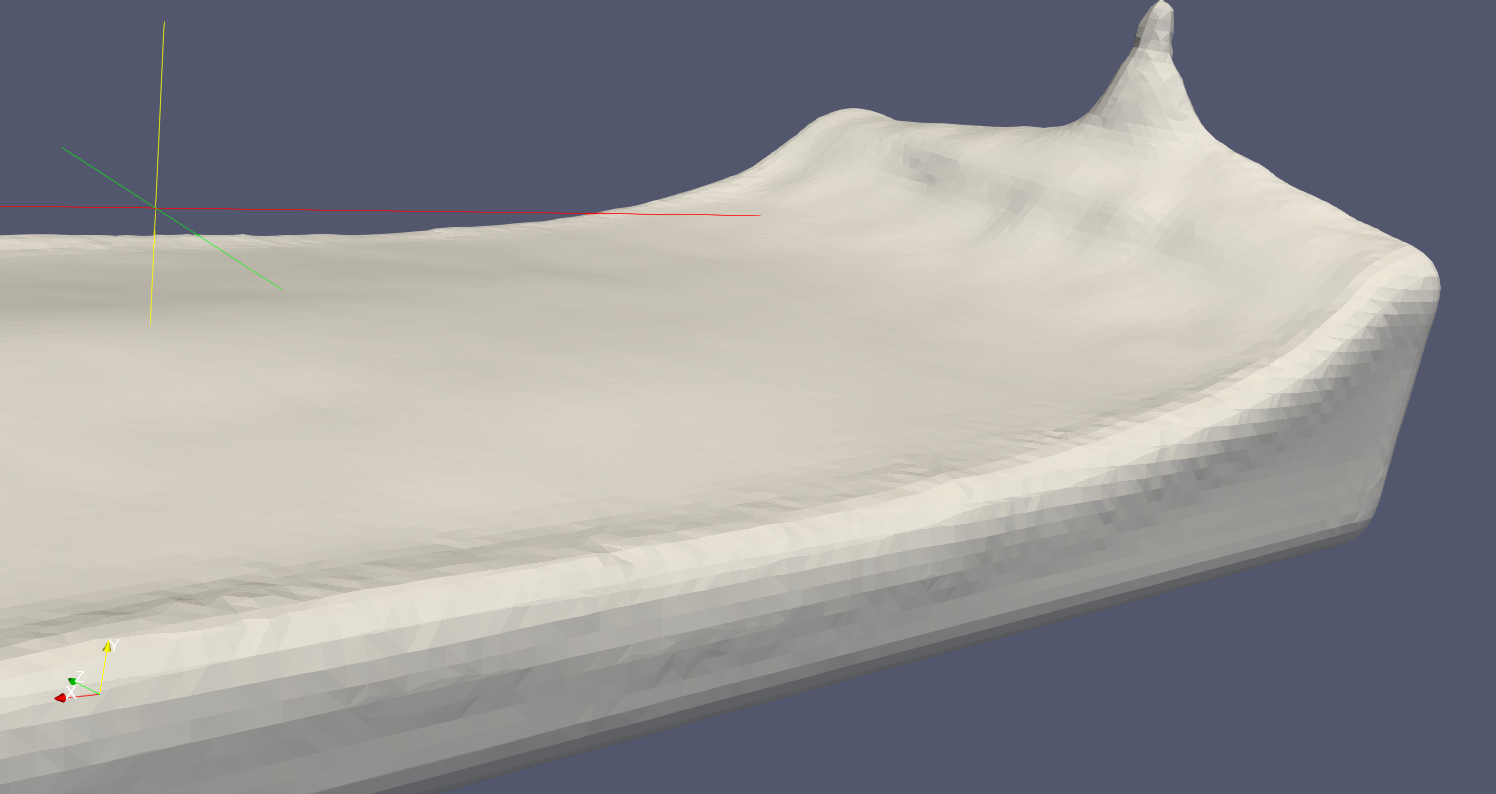
\includegraphics[width=\textwidth]{figures/MLSSurfaceSamplingQuarterSet.png}
			\caption{mls corrected surface with quarter set of samples}
		\end{subfigure}
	\end{center}
	\caption{Reconstructed mls surface} \label{fig:surface_sampling_results}
\end{figure}
Both, full samples set and partial samples set removes bumps from the original surface, but for the reconstruction with $\dfrac{1}{4}$ set of mls samples small frequency noise can be seen on the corner areas.\\

\subsection{Clusters density factor}
According to the algorithm \ref{alg:mls_alg} clusters are computed for each 0-level intersection cell, and after this mls approximation is applied to each intersection cell in the cluster. This means that each 0-level intersection MC vertex takes part in multiple clusters during the mls approximation. However, for fluid surface smoothing it is enough to generate clusters only for a subset of the 0-level intersection cells such that depending on the size of the cluster all 0-level intersection vertices will be mls corrected. For example see figure \ref{fig:mls_clusters_sparse_generations}:
\begin{figure}[H]
	\begin{center}
		\begin{subfigure}[b]{0.48\textwidth}
			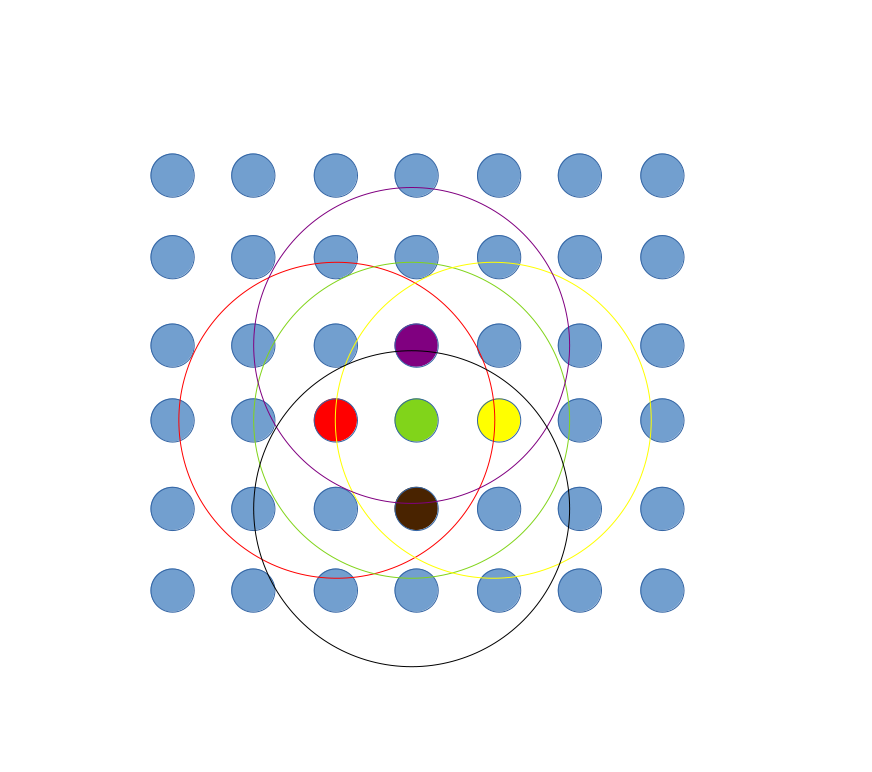
\includegraphics[width=\textwidth]{figures/FullDomainClusters.png}
			\caption{} \label{fig:mls_clusters_sparse_generations_nonsparse}
		\end{subfigure}
		\begin{subfigure}[b]{0.48\textwidth}
			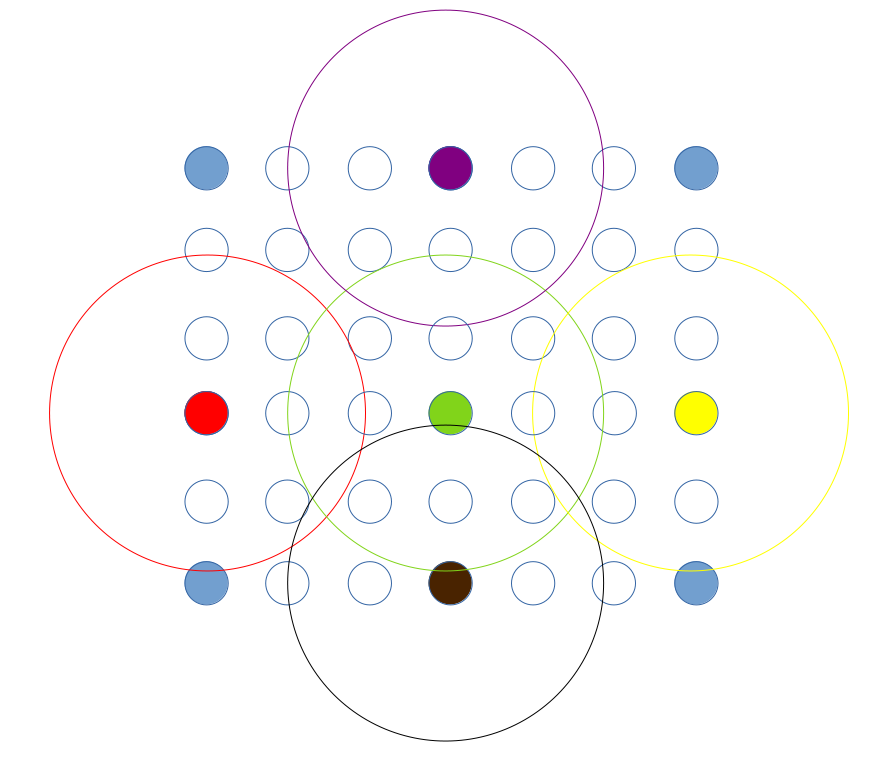
\includegraphics[width=\textwidth]{figures/PartialDomainClusters.png}
			\caption{} \label{fig:mls_clusters_sparse_generations_sparse}
		\end{subfigure}
	\end{center}
	\caption{Comparison of sparse and non sparse clusters computation.} \label{fig:mls_clusters_sparse_generations}
\end{figure} 
Filled vertices are the MC grid vertices for which clusters are generated, and then mls correction is computed. Generating clusters for each 0-level intersection cell might be redundant, thus clusters can be computed not for all domain of 0-level intersection vertices but just for a subset of the 0-level intersection vertices domain (see figure \ref{fig:mls_clusters_sparse_generations_nonsparse}). However, it is important to generate clusters such that they overlap, while for different clusters different surface approximations is computed and thus in the border areas non-smooth transitions can be observed. To accomplish this problem ClusterFactor ($cf$) is used. ClusterFactor identifies the fraction of the 0-level intersection vertices for which clusters will be computed. For simplicity $cf \cdot n$ out of $n$ 0-level intersection vertices will be picked uniformly at random. Figure \ref{fig:mls_sparse_clusters_reconstruction} shows the results of the reconstruction given different valuations of $ClusterFactor$.
\begin{figure}[H]
	\begin{center}
		\begin{subfigure}[b]{0.46\textwidth}
			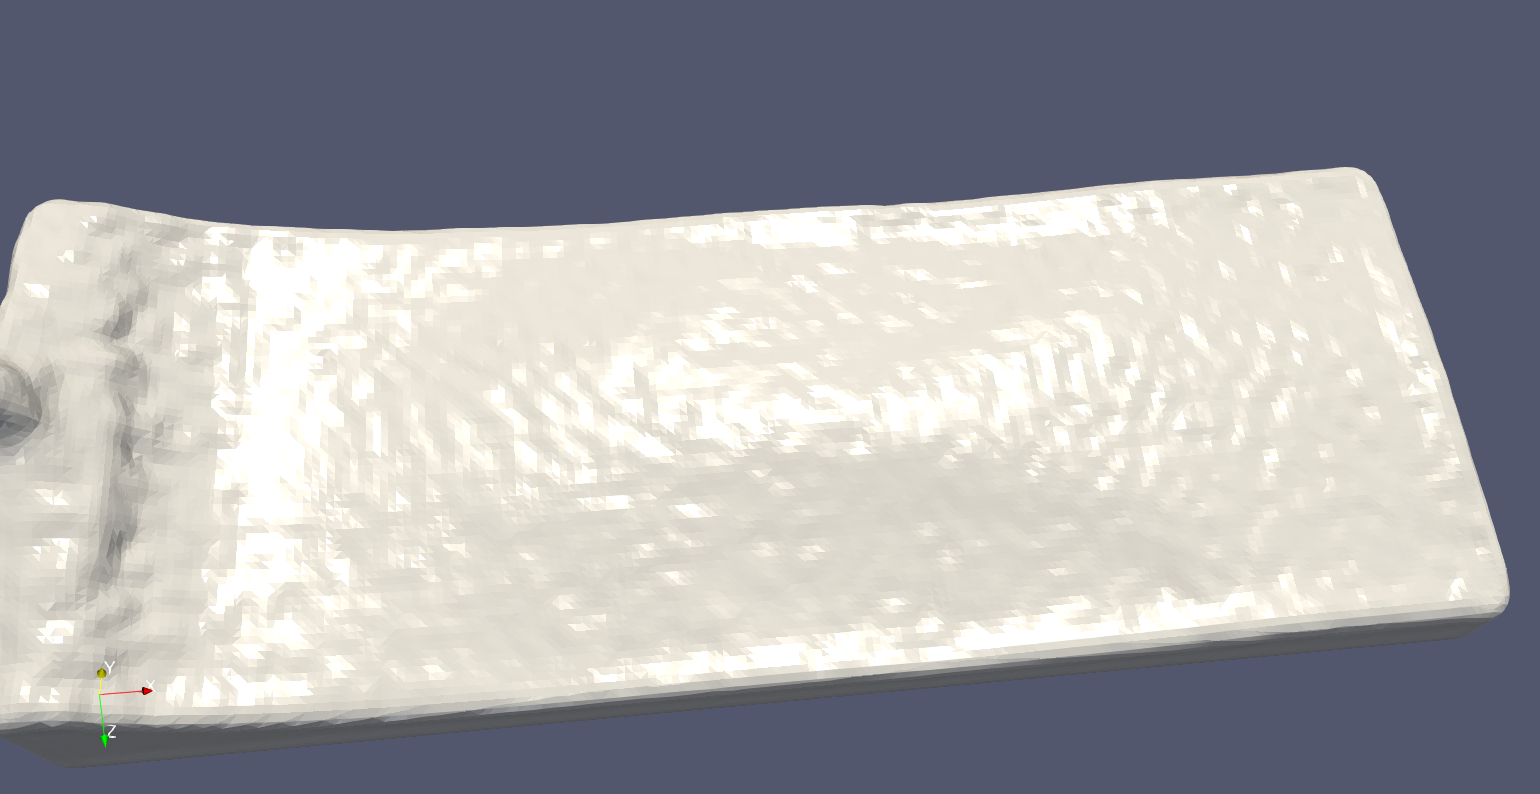
\includegraphics[width=\textwidth]{figures/MlsSparseClustersOriginalpng.png}
			\caption{Original reconstruction} \label{fig:mls_clusters_original}
		\end{subfigure}
		\begin{subfigure}[b]{0.46\textwidth}
			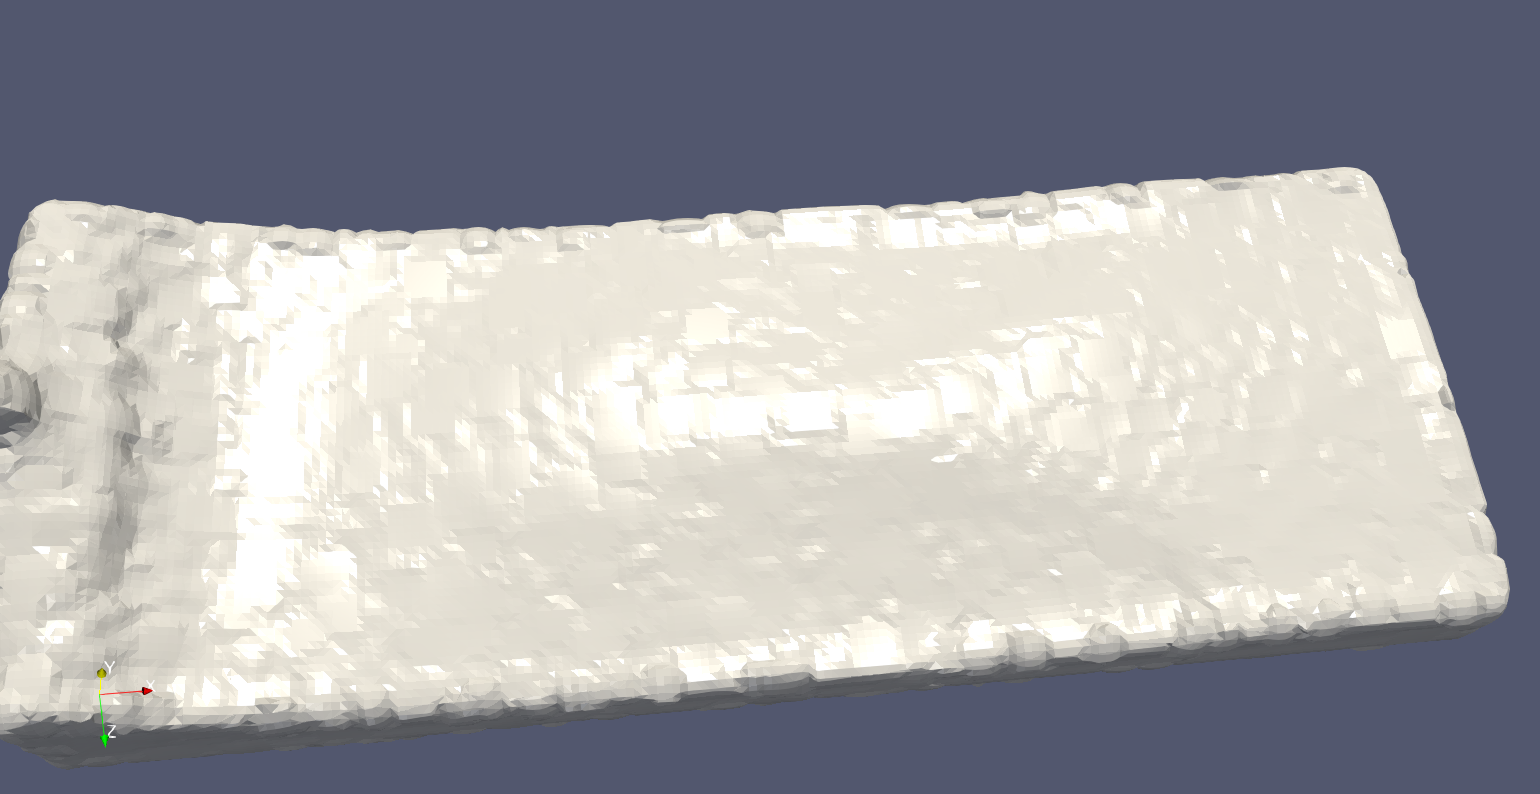
\includegraphics[width=\textwidth]{figures/MlsSparseClusters0.01.png}
			\caption{ClusterFactor = 0.01} \label{fig:mls_clusters_sparse_0.01}
		\end{subfigure}
		\begin{subfigure}[b]{0.46\textwidth}
			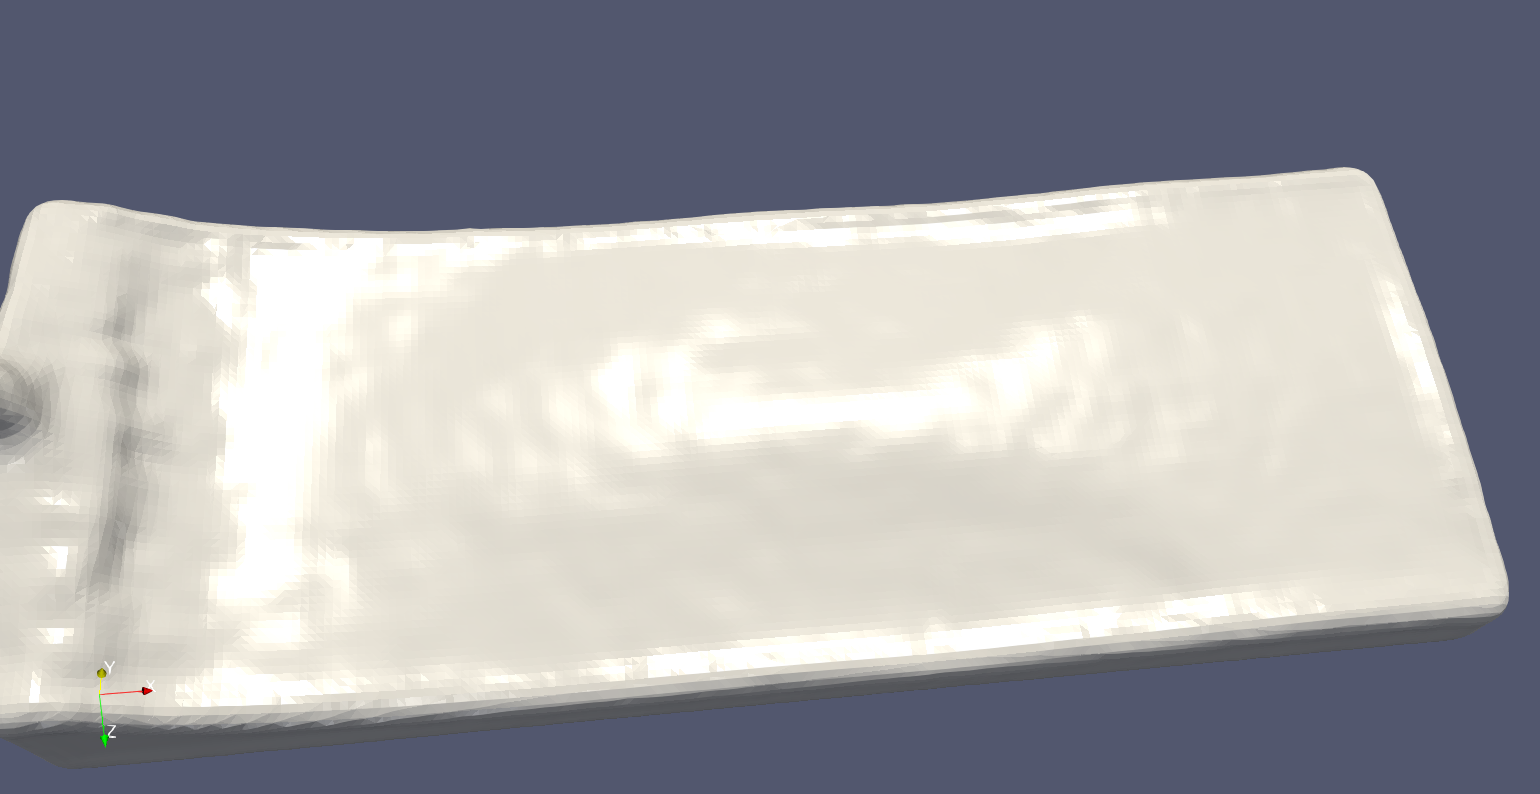
\includegraphics[width=\textwidth]{figures/MlsSparseClusters0.5.png}
			\caption{ClusterFactor = 0.5} \label{fig:mls_clusters_sparse_0.5}
		\end{subfigure}
		\begin{subfigure}[b]{0.46\textwidth}
			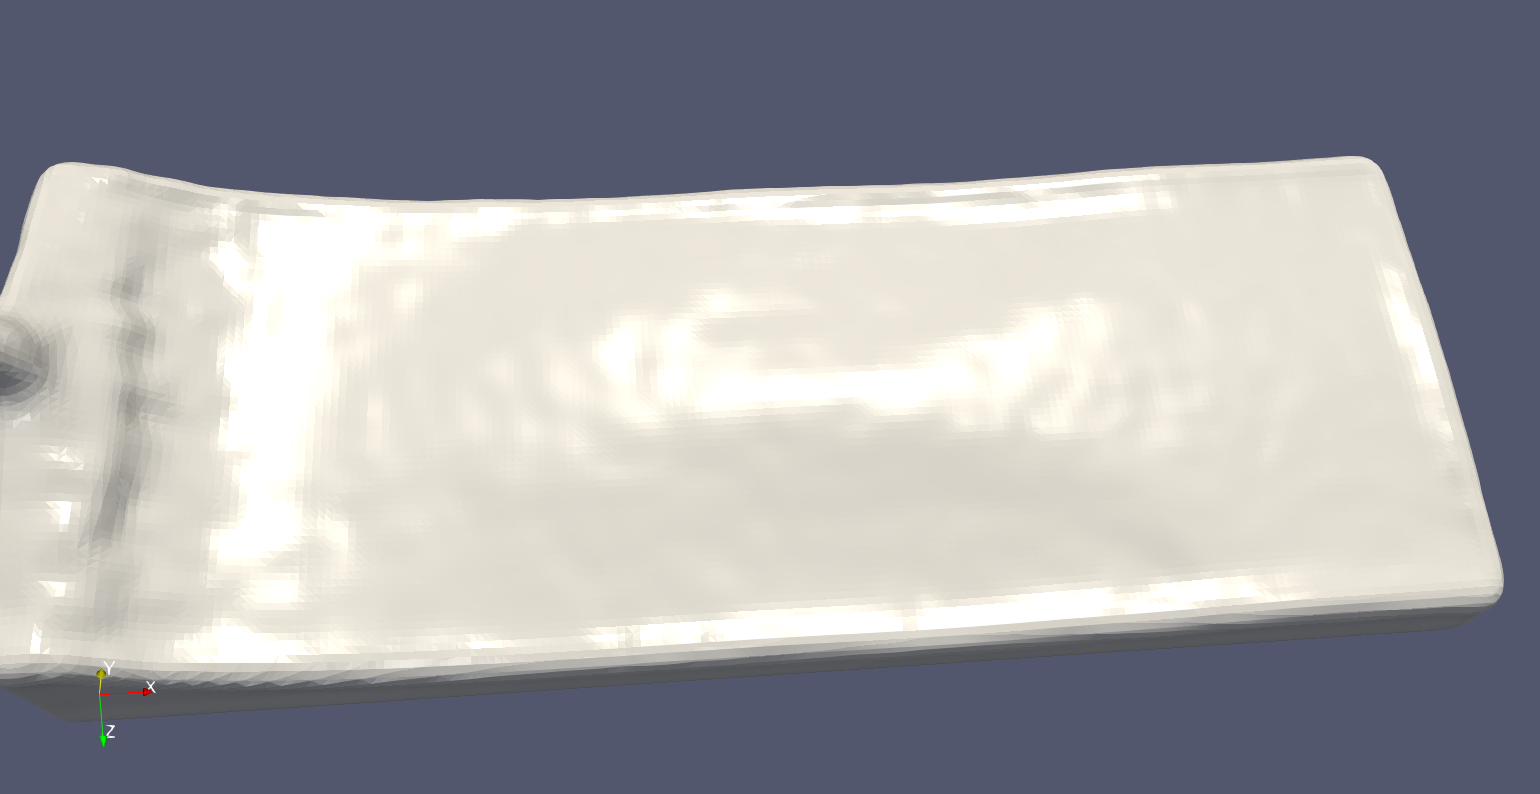
\includegraphics[width=\textwidth]{figures/MlsSparseClusters1.png}
			\caption{ClusterFactor = 1} \label{fig:mls_clusters_sparse_1}
		\end{subfigure}

	\end{center}
	\caption{Comparison reconstruction which uses full domain of 0-level intersection cells for clusters computation and subset of 0-level intersection cells depending on the ClusterFactor.} \label{fig:mls_sparse_clusters_reconstruction}
\end{figure} 
Taking into account that the number of mls vertices in the cluster is 100, mls smoothing over the 0-level intersection vertices with ClusterFactor 0.01 is generating clusters without overlap, thus on the figure \ref{fig:mls_clusters_sparse_0.01} the reconstructed surface looks such as if the surface was built from parts of spheres. In the other hand taking $ClusterFactor = 0.5$ reconstructed surface looks much smoother (see figure \ref{fig:mls_clusters_sparse_0.5}). In this thesis $ClusterFactor = 0.5$ was used for reconstruction of fluid surfaces. 

\subsection{Mls surface computation}

The core of the smoothing method is a computation of an approximated surface. 
The main idea of computational approach was taken from the work of Guennebaud \& Gross \cite{Apss}. 
Given a set of points $P = \{p_i \in R_d \}$, a smooth surface $S_P$ approximating $P$ using a moving least squares spherical fit to the data can be defined. However, in case of this study there is no set of points, that define surface and which should be approximated. As an input we receive a set of points, that are resided near the surface - e.g. the MC grid vertices, that are resided in the nearest neighborhood to the 0-level iso-surface. 
Although, with the MC grid vertices we also have a values of the SDF, which theoretically define the distance to the surface. But in most cases the computed SDF doesn't represent an actual distance to the surface, but just an approximation of the distance, which is more approximate in the neighborhood of the 0-level iso-surface, but is not define the distance to the surface in the further areas of the fluid. 
However, in the 0-level intersection areas SDF also doesn't exactly defines a distance to the surface, which is one of the reason of the occurrence of small frequency bubs on the reconstructed fluid surface. Thus applying mls approximation to the 0-level intersection MC vertices and correcting their SDF is an attempt to reconstruct a smooth distance based SDF.\\
In the APSS work analytical equation of the sphere was used as a core function, that is approximated by applying least squares approximation to a samples set. Given a point $x$ the equation, that represents a distance to the sphere center can be represented as a function of x:
\begin{equation}
f(x) = s_1\cdot x^2 + s_2 \cdot x_x + s_3 \cdot x_y + s_4 \cdot x_z + s_5
\end{equation}
where $x^2$ is a dot product of point $x$ on itself, $s_i$ are unknown coefficients, that are going to be calculated. Thus the goal is to calculate the unknown coefficients $s_i$, and based to the approximated mls surface correct the sdf value by multiplying the MC grid vertex world coordinate by the coefficients:
\begin{equation}
SDF_{new}(x_i) = f(x_i) = s_1\cdot x_i^2 + s_2 \cdot x_{i_x} + s_3 \cdot x_{i_y} + s_4 \cdot x_{i_z} + s_5
\end{equation}
In the Algorithm \ref{alg:mls_alg} each MC grid vertex in the cluster $SDF_{new}$ is computed. As soon as each particle can appear in the cluster multiple times for each cluster, for which mls corrected surface is computed. Then the final SDF is a weighted sum of all sdf's, computed according to the Algorithm \ref{alg:mls_alg}, divided by total sum of weights:
\begin{equation}
	SDF_{mls}(x) = \dfrac{\sum_{j \in Clusters}{SDF_{new_j}(x)}}{|Clusters|}
\end{equation}
where $Clusters$ is a set of clusters, such that $: \forall cluster \in Clusters: x \in cluster$. 
\subsection{Applying mls filter iteratively}
In the Algorithm \ref{alg:mls_alg} it is stated that only computed 0-level intersection MC grid vertices are under the mls correction procedure. In the meantime the MC grid vertices, that are not taking part in surface mesh generation while cells no neighbor vertices contains SDF value transfer from positive to negative and vice-verse, thus the SDF correction procedure is not applied to this vertices. In this case next problem can arise: the corrected MC vertices can change the sign of SDF and will be no more in a subset of the 0-level intersection MC grid vertices, and non corrected vertices, that are in the neighborhood of the stated vertices, will not take part in surface generation. In the Figure \ref{fig:mls_iterations} shown the effect of applying mls correction on the 0-level intersection MC grid vertices:
\begin{figure}[H]
	\begin{center}
		\begin{subfigure}[b]{0.9\textwidth}
			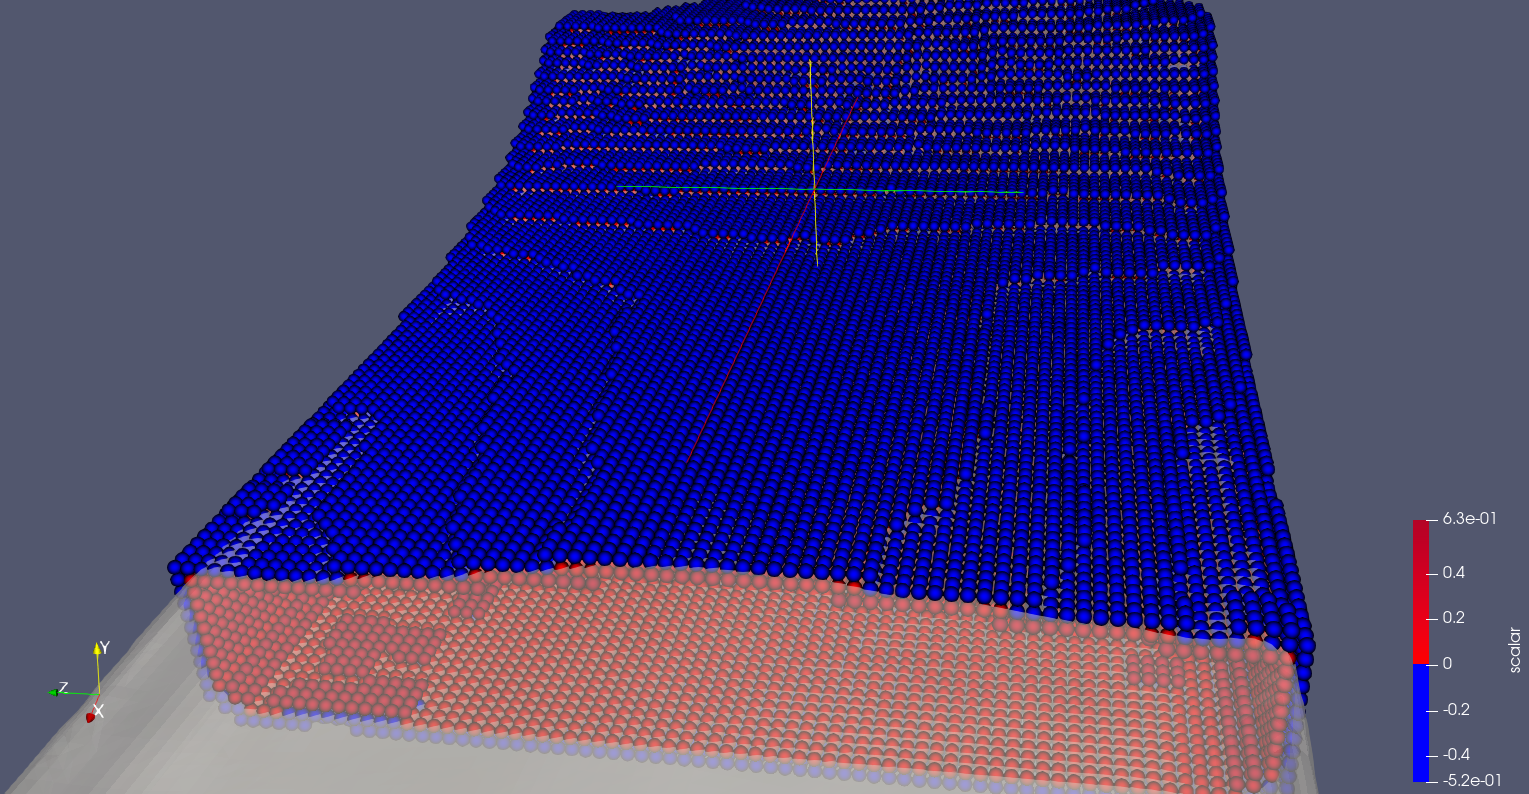
\includegraphics[width=\textwidth]{figures/IntersectionCellsSdfBeforeMls_1_iter.png}	
			\caption{Before mls smoothing} \label{fig:mls_0_iter}
		\end{subfigure}
		\begin{subfigure}[b]{0.9\textwidth}
			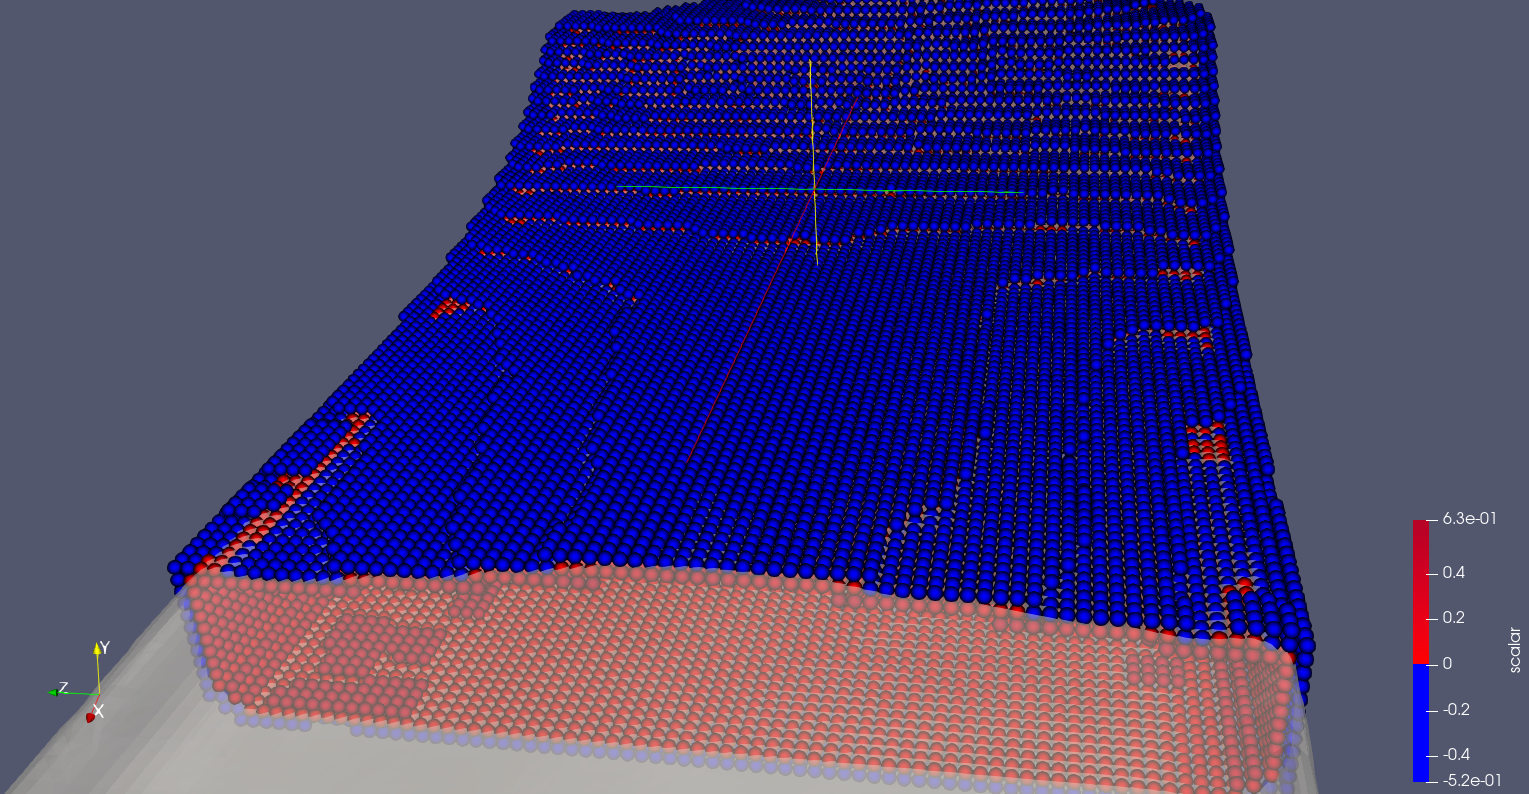
\includegraphics[width=\textwidth]{ figures/IntersectionCellsSdfAfterMls_1_iter.png}	
			\caption{1 iterations of mls smoothing} \label{fig:mls_1_iter}
		\end{subfigure}
		\begin{subfigure}[b]{0.9\textwidth}
			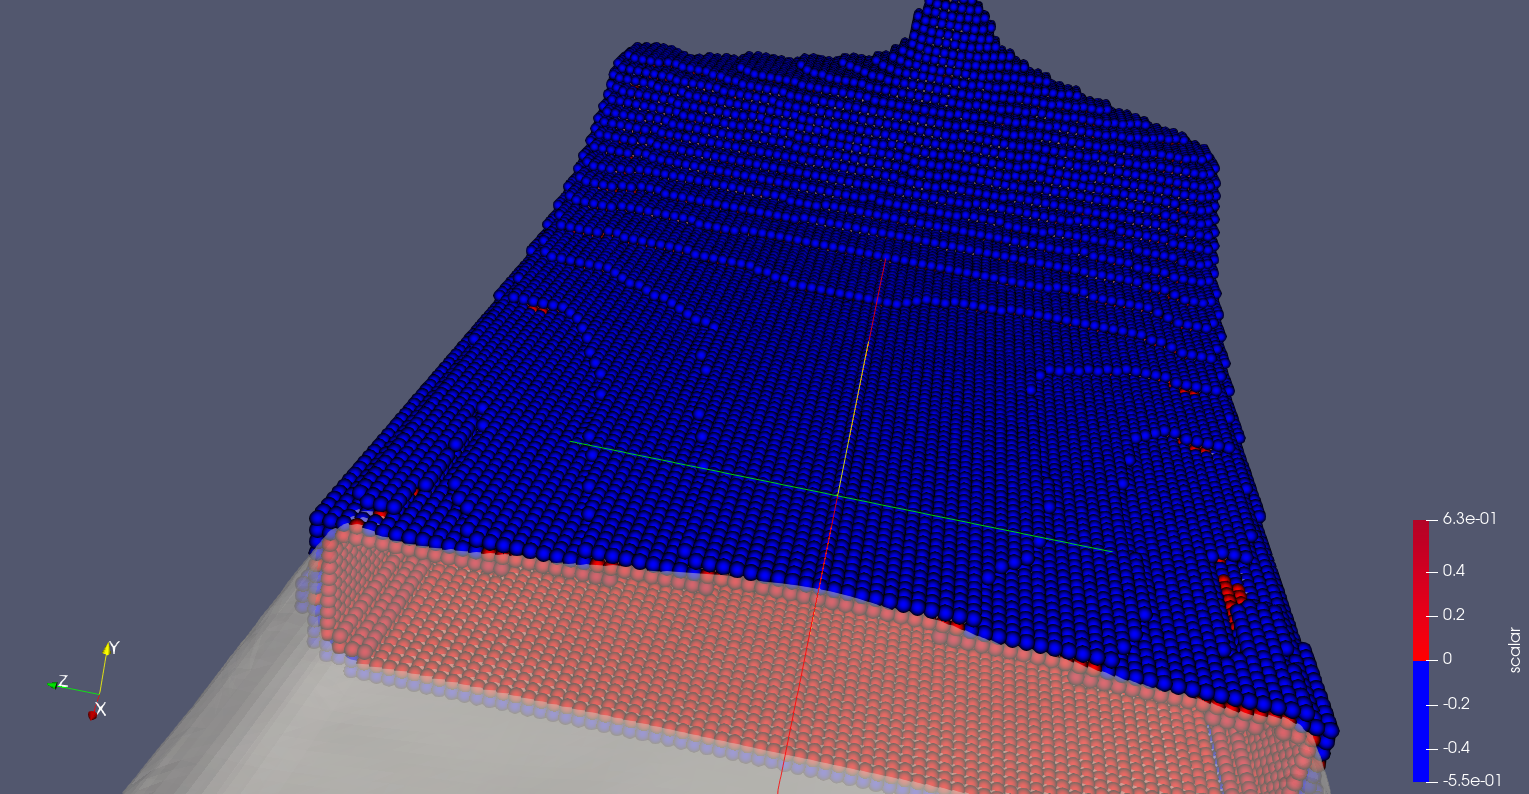
\includegraphics[width=\textwidth]{figures/IntersectionCellsSdfAfterMls_3_iter.png}	
			\caption{3 iterations of mls smoothing} \label{fig:mls_3_iter}
		\end{subfigure}
	\end{center}
	\caption{Subset of 0-level intersection MC grid vertices with SDF values before and after mls smoothing. Red are vertices with positive SDF valuations, blue are vertices with negative SDF value.} 
	\label{fig:mls_iterations}
\end{figure}
After application of mls it can be seen on the picture, that some MC grid vertices changed its SDF sign from negative to positive (Figure \ref{fig:mls_1_iter}). After 3 iterations of mls filter smoothing the effect of SDF sign switch is applied to smaller subset of MC grid vertices (Figure \ref{fig:mls_3_iter}). This can be explained by the convergence of the surface to some invariant state, since each iteration the average standard deviation of SDF values before and after the application of MLS among all clusters gradually decreases and converges to 0:
\begin{figure}[H]
	\begin{center}
		\begin{tikzpicture}
			\begin{axis}
				[
					xlabel=iterations,
					ylabel=error,
					width = 0.45\textwidth
				]
				\addplot[
					red,
					mark=*
				] table{mls_std_dev.txt};
			\end{axis}
		\end{tikzpicture}
	\end{center}
	\caption{Total standard deviation of each grid vertex's SDF before and after mls correction}
	\label{fig:mls_std_dev}
\end{figure}
There are some examples of reconstructed surface shown in the Figure \ref{fig:mls_surf_iter_examples} and \ref{fig:mls_surf_iter_examples2} given different amount of iterations.
\begin{figure}
	\begin{center}
		\begin{subfigure}[b]{0.47\textwidth}
			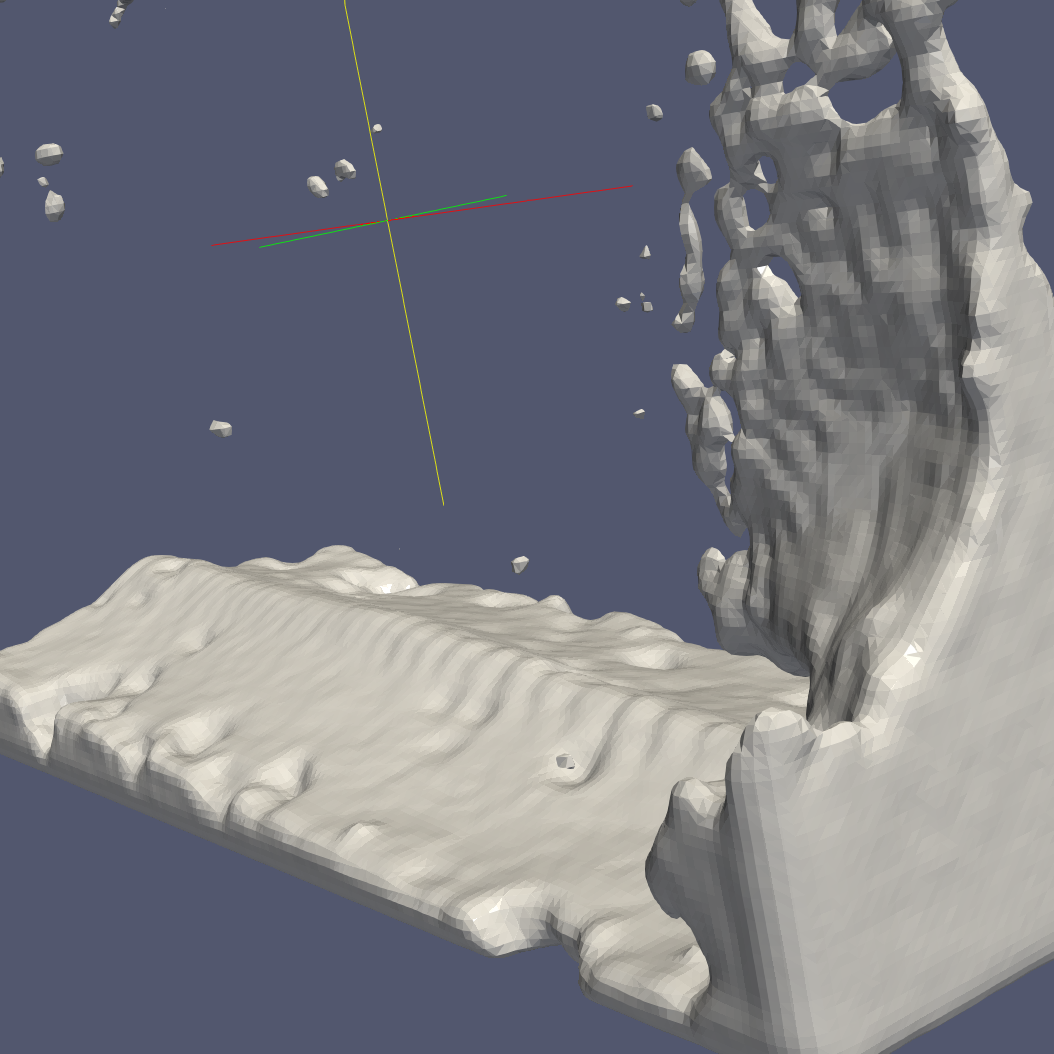
\includegraphics[width=\textwidth]{figures/MlsSurfaceInitial.png}
			\caption{original surface}
		\end{subfigure}
		\begin{subfigure}[b]{0.47\textwidth}
			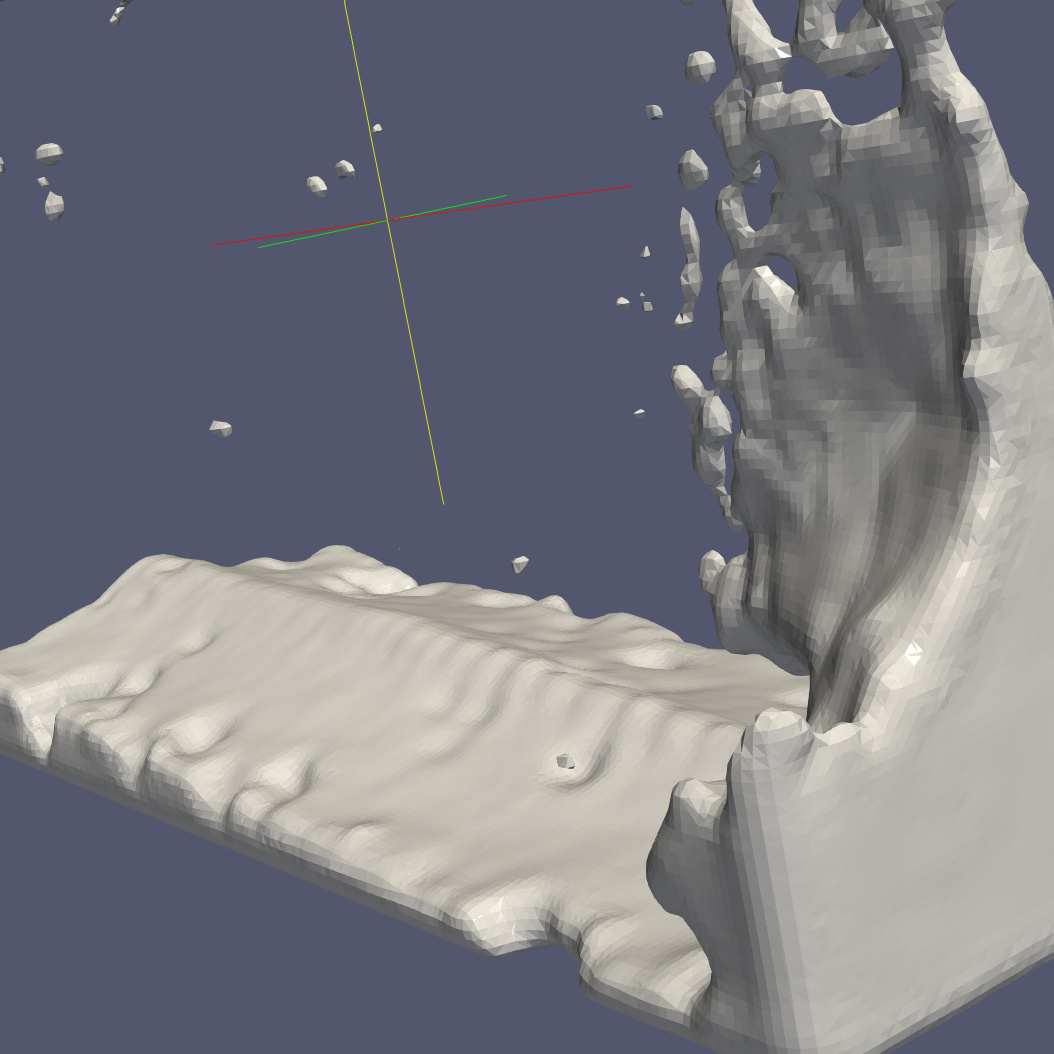
\includegraphics[width=\textwidth]{figures/MlsSurface1Iteration.png}
			\caption{Mls correction 1 iteration}
		\end{subfigure}
		\begin{subfigure}[b]{0.47\textwidth}
			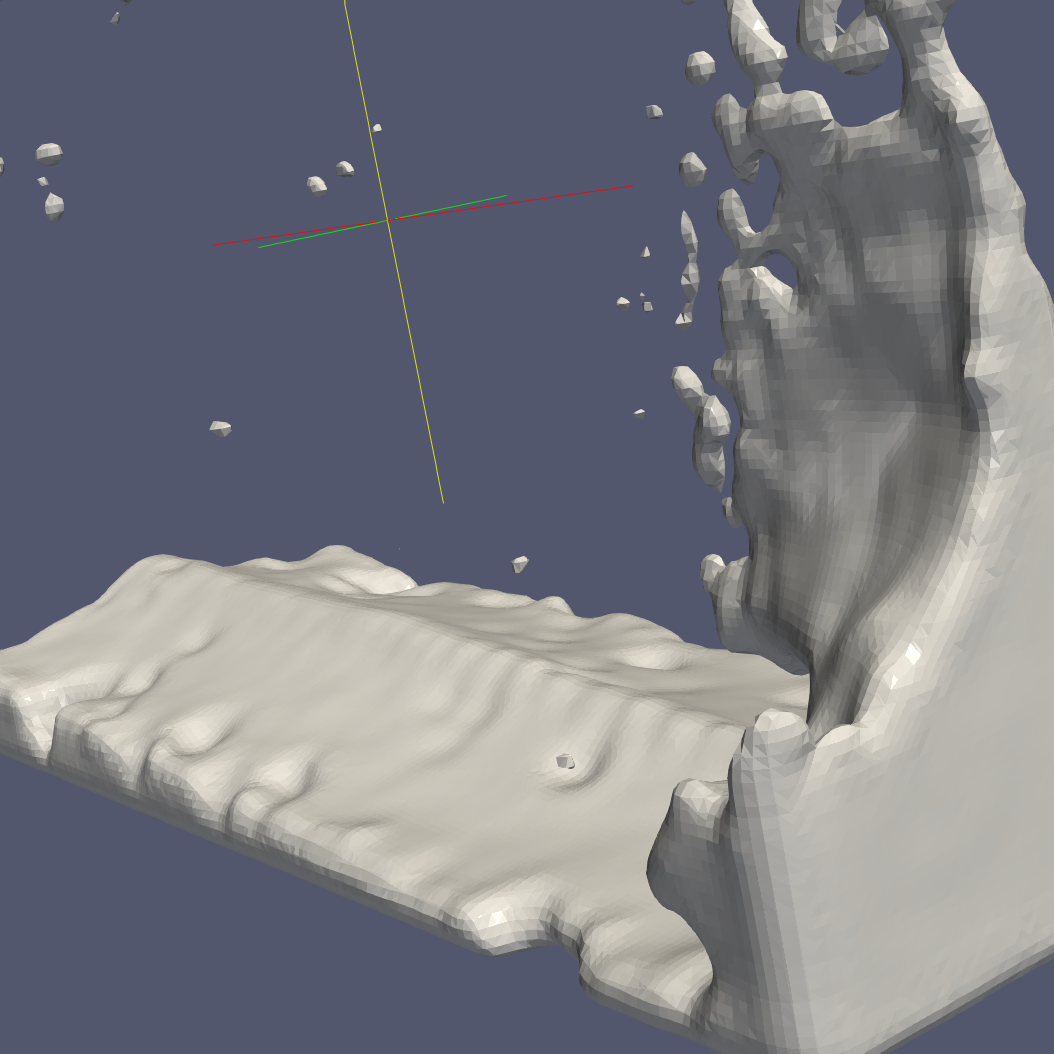
\includegraphics[width=\textwidth]{figures/MlsSurface2Iteration.png}
			\caption{Mls correction 2 iterations}
		\end{subfigure}
		\begin{subfigure}[b]{0.47\textwidth}
			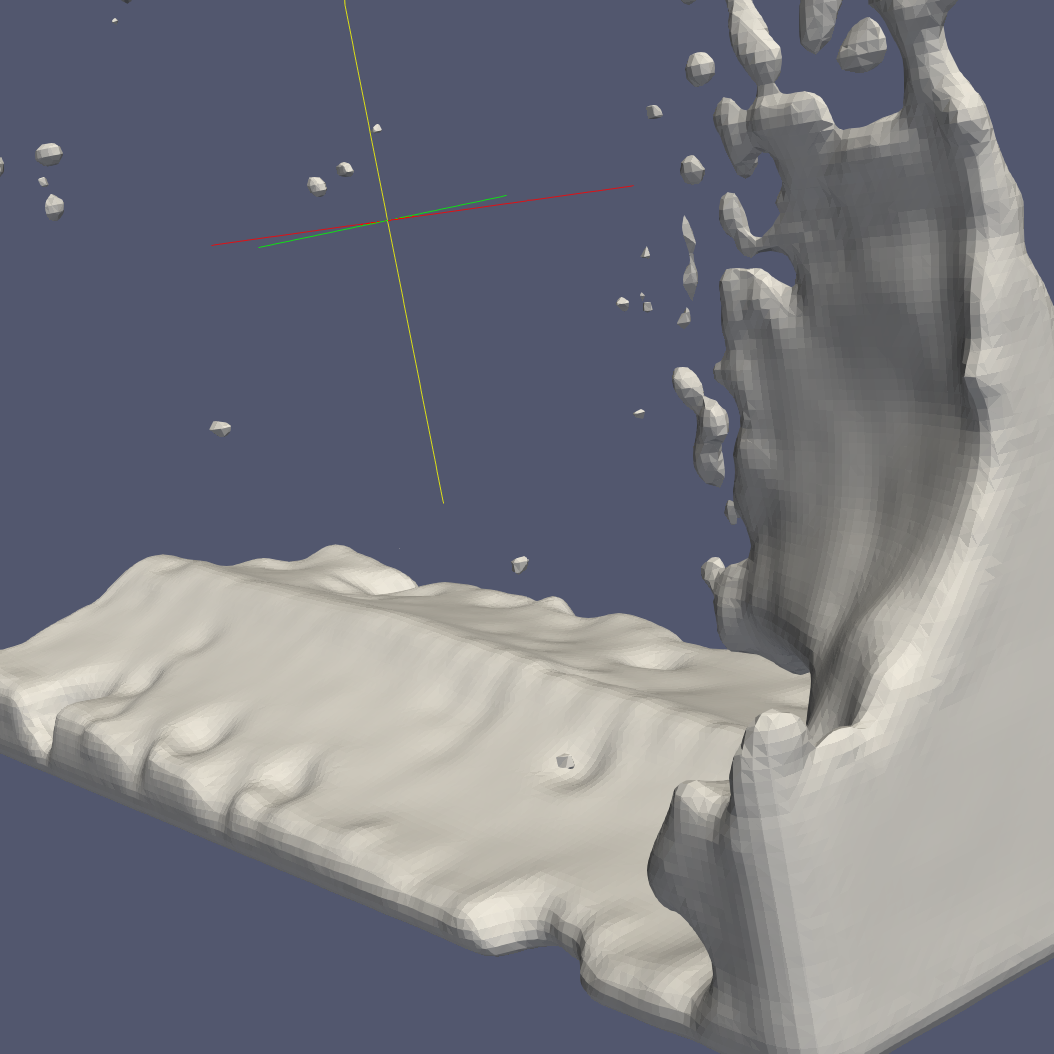
\includegraphics[width=\textwidth]{figures/MlsSurface3Iteration.png}
			\caption{Mls correction 3 iterations}
		\end{subfigure}
		\begin{subfigure}[b]{0.47\textwidth}
			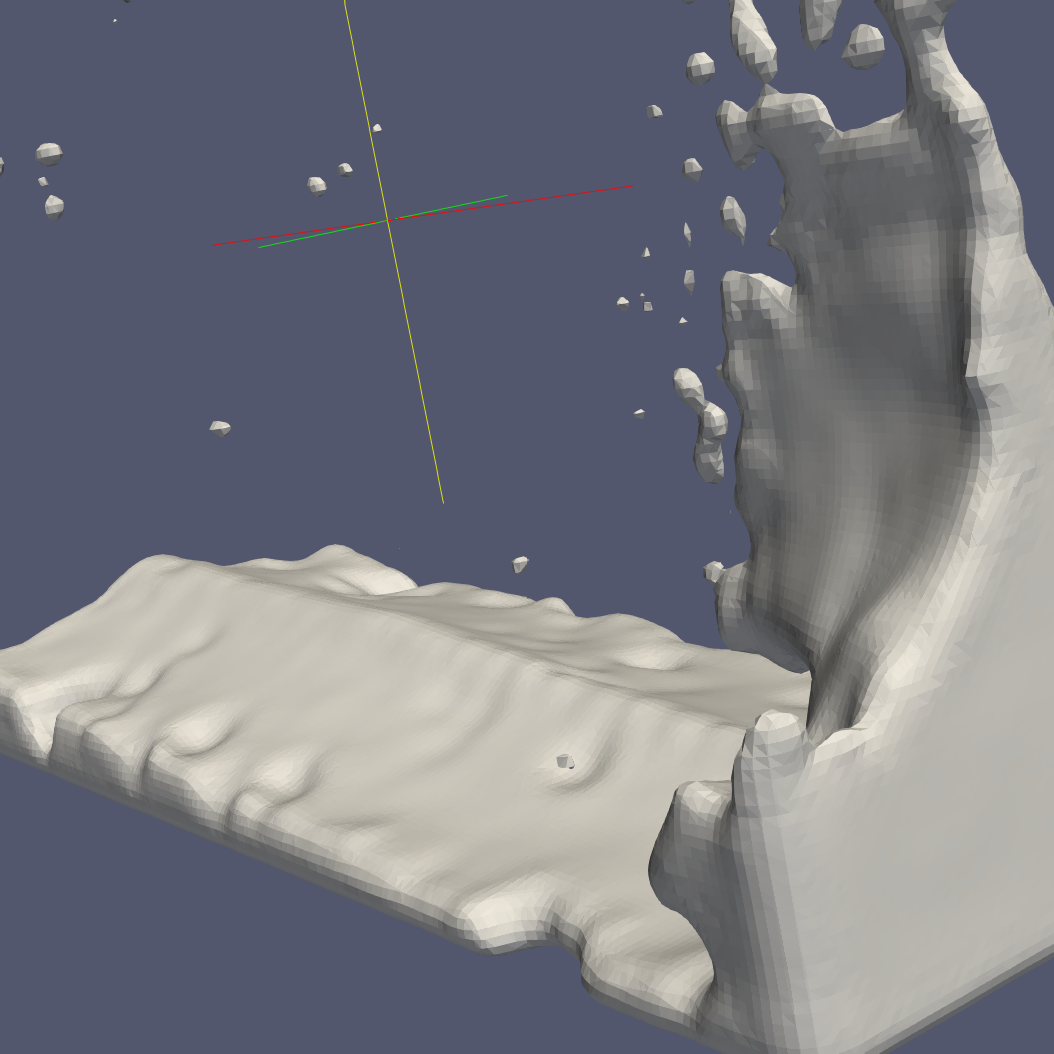
\includegraphics[width=\textwidth]{figures/MlsSurface4Iteration.png}
			\caption{Mls correction 4 iterations}
		\end{subfigure}
		\begin{subfigure}[b]{0.47\textwidth}
			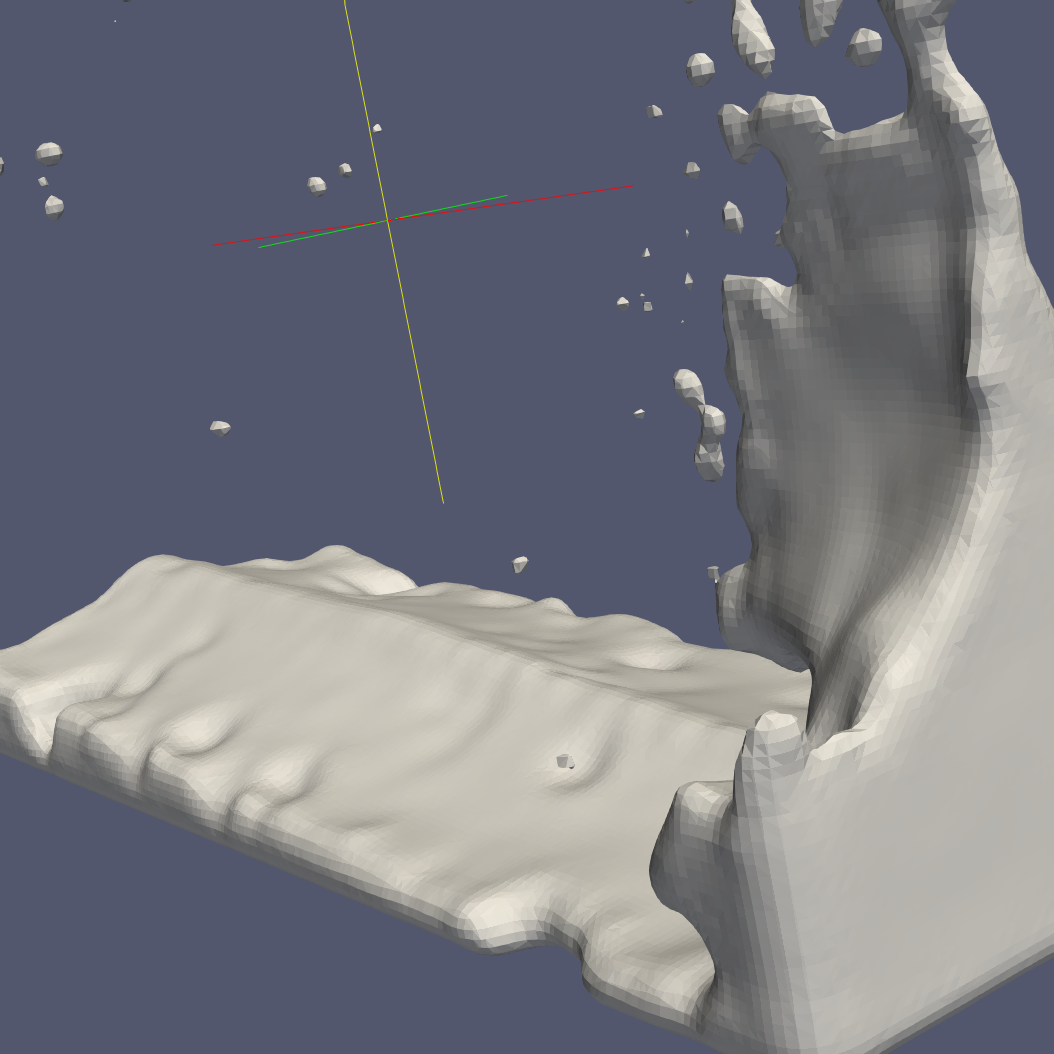
\includegraphics[width=\textwidth]{figures/MlsSurface5Iteration.png}
			\caption{Mls correction 5 iterations}
		\end{subfigure}
	\end{center}
	\caption{Reconstructed mls surface} \label{fig:mls_surf_iter_examples}
\end{figure}
\begin{figure}
	\begin{center}
		\begin{subfigure}[b]{0.47\textwidth}
			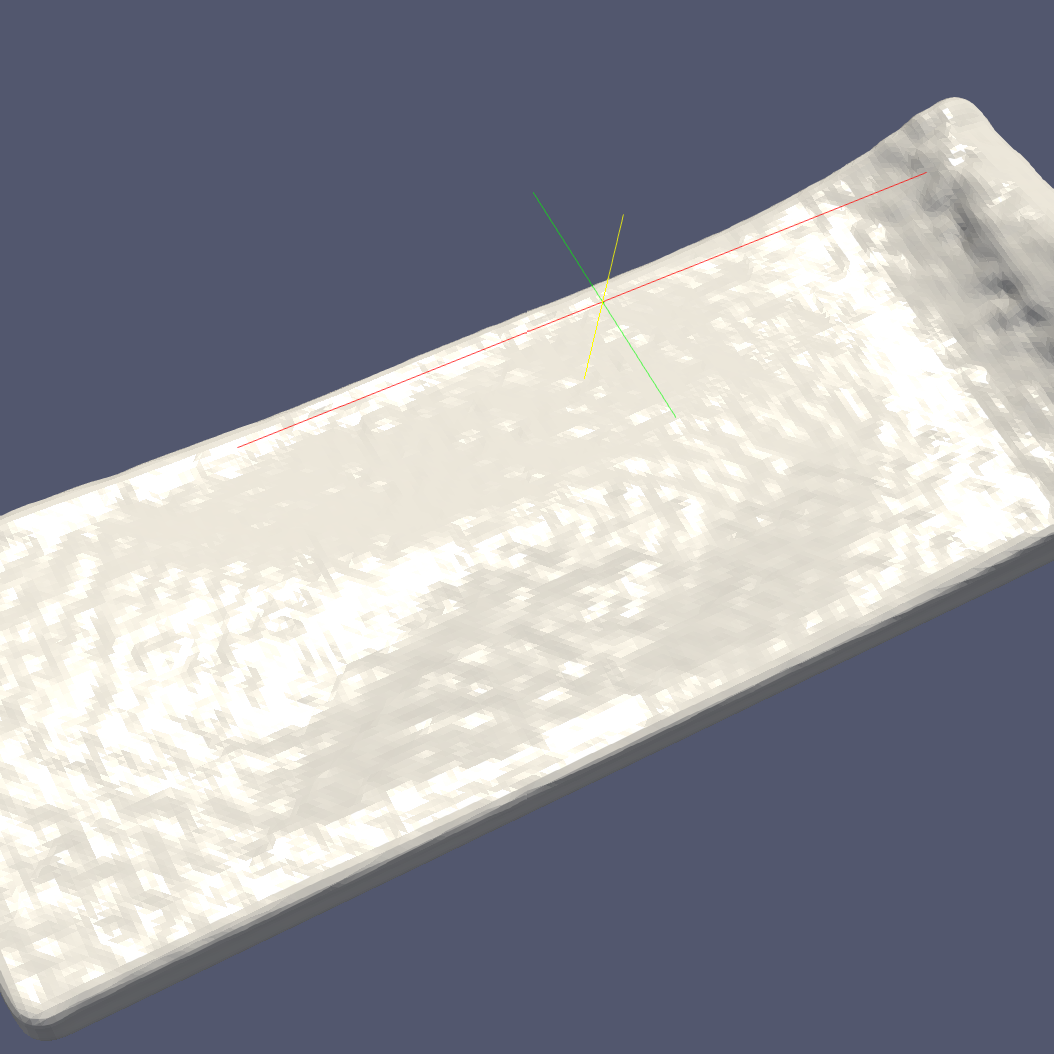
\includegraphics[width=\textwidth]{figures/MLS2SurfaceOriginal.png}
			\caption{original surface}
		\end{subfigure}
		\begin{subfigure}[b]{0.47\textwidth}
			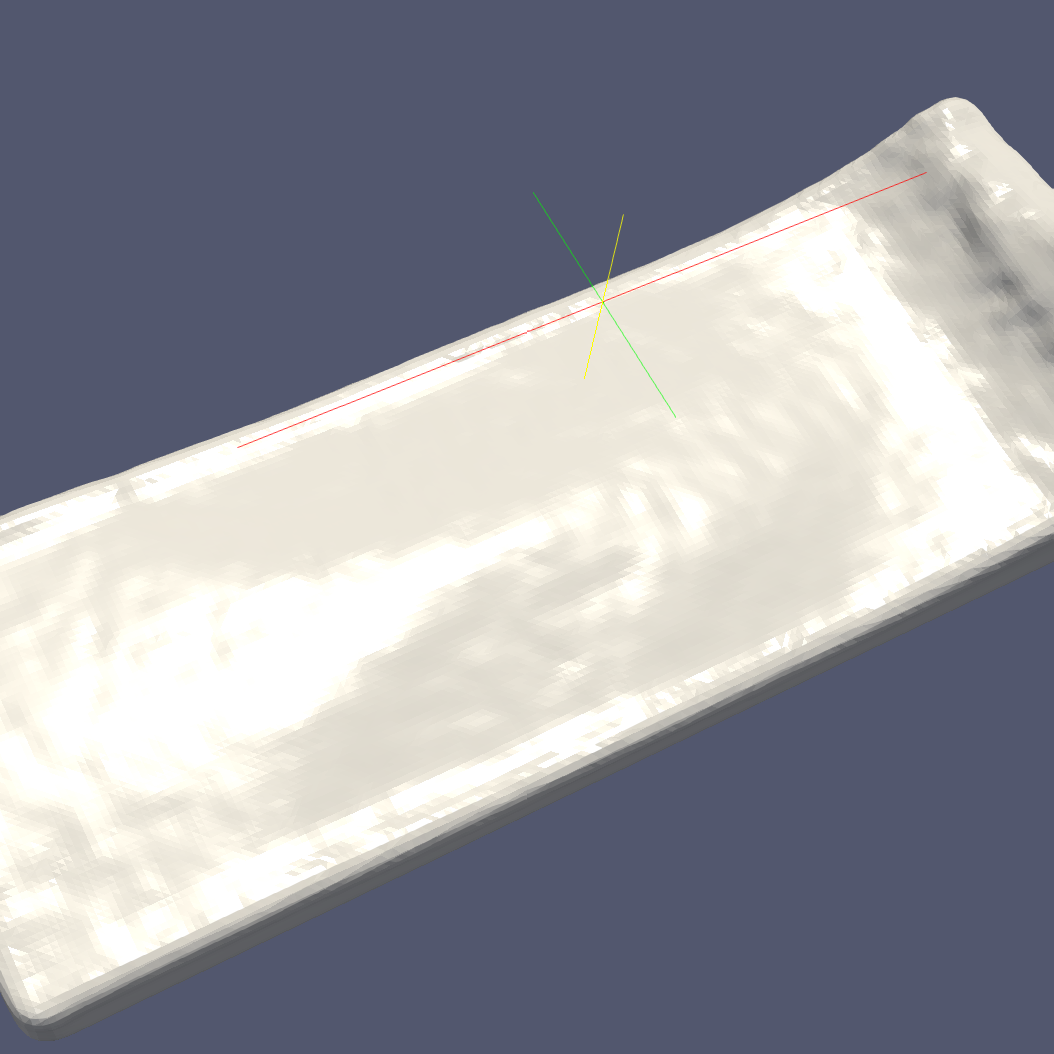
\includegraphics[width=\textwidth]{figures/Mls2Surface1Iteration.png}
			\caption{Mls correction 1 iteration}
		\end{subfigure}
		\begin{subfigure}[b]{0.47\textwidth}
			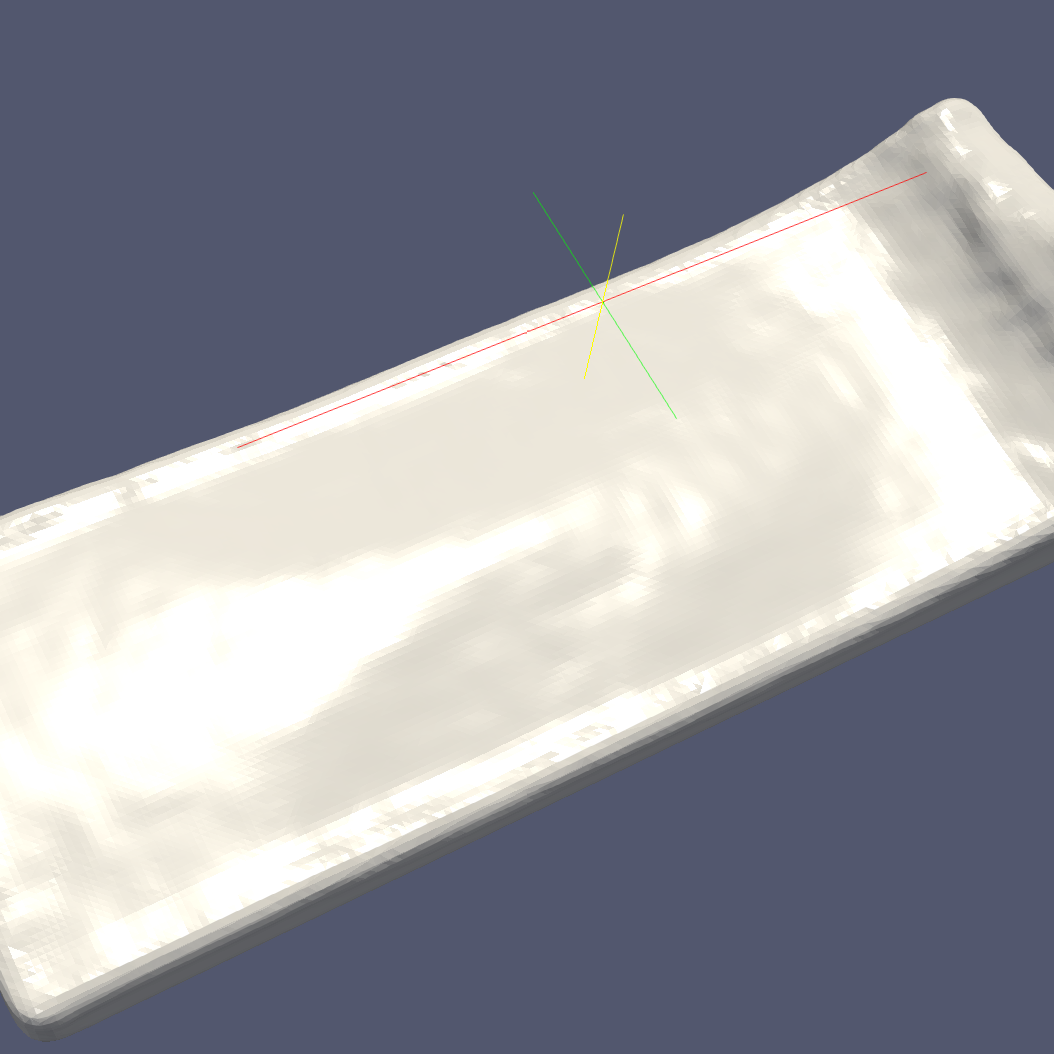
\includegraphics[width=\textwidth]{figures/Mls2Surface2Iteration.png}
			\caption{Mls correction 2 iterations}
		\end{subfigure}
		\begin{subfigure}[b]{0.47\textwidth}
			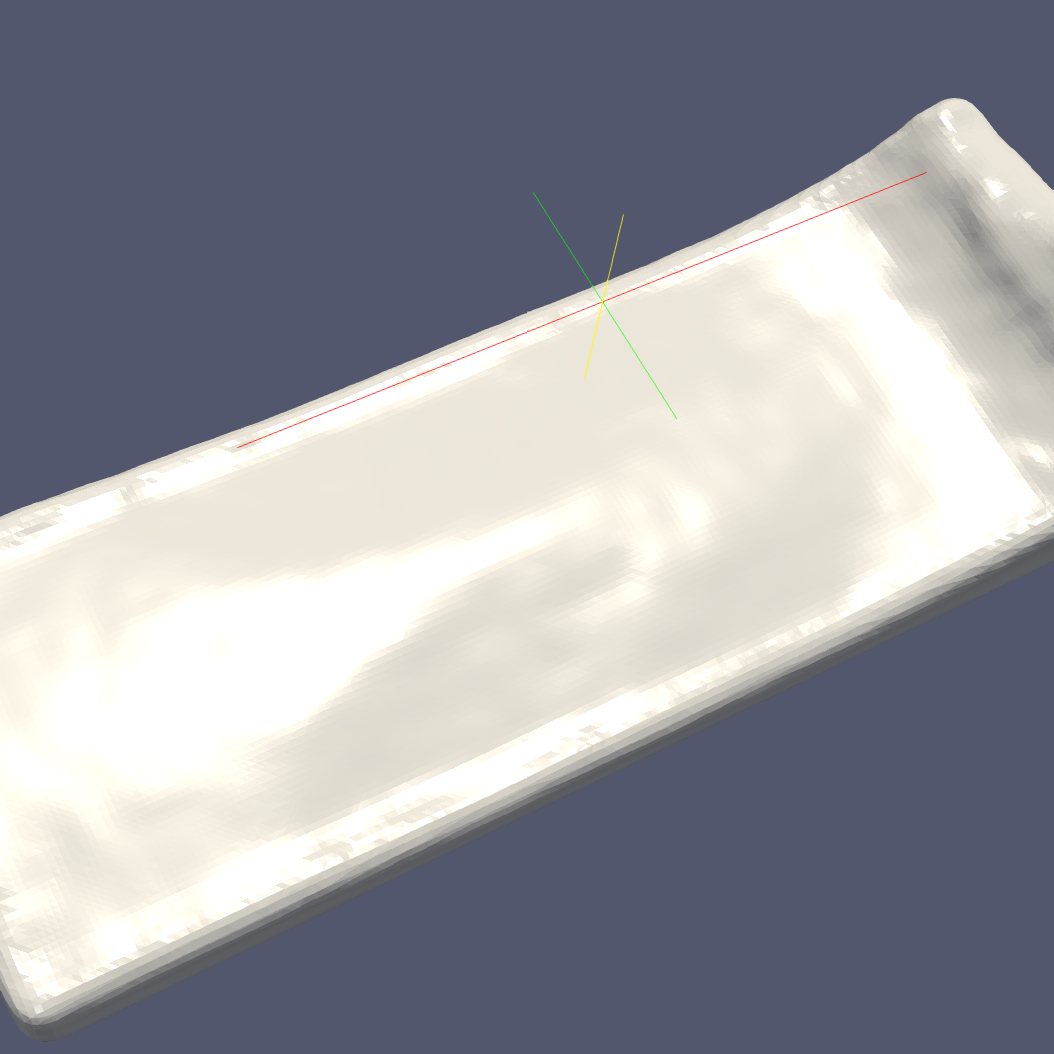
\includegraphics[width=\textwidth]{figures/Mls2Surface3Iteration.png}
			\caption{Mls correction 3 iterations}
		\end{subfigure}
		\begin{subfigure}[b]{0.47\textwidth}
			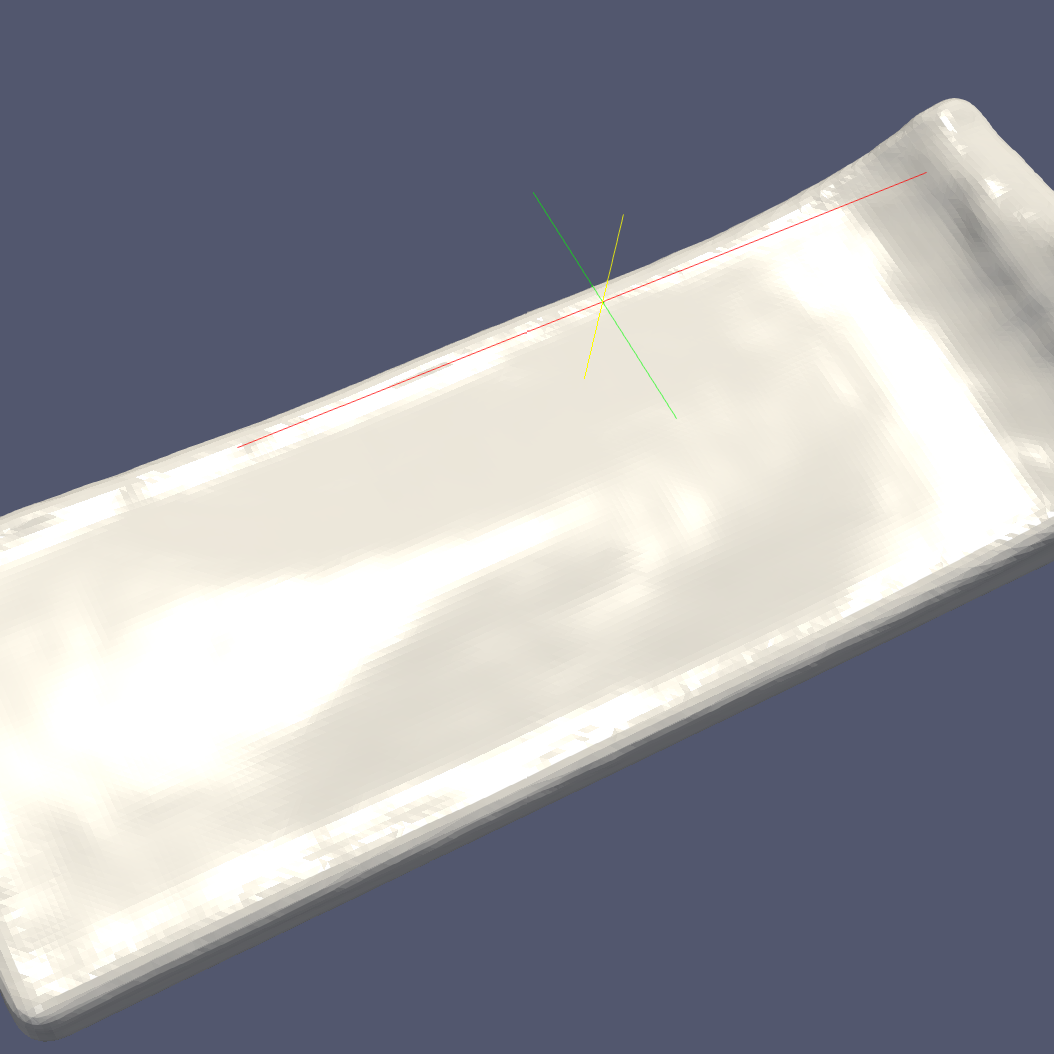
\includegraphics[width=\textwidth]{figures/Mls2Surface4Iteration.png}
			\caption{Mls correction 4 iterations}
		\end{subfigure}
		\begin{subfigure}[b]{0.47\textwidth}
			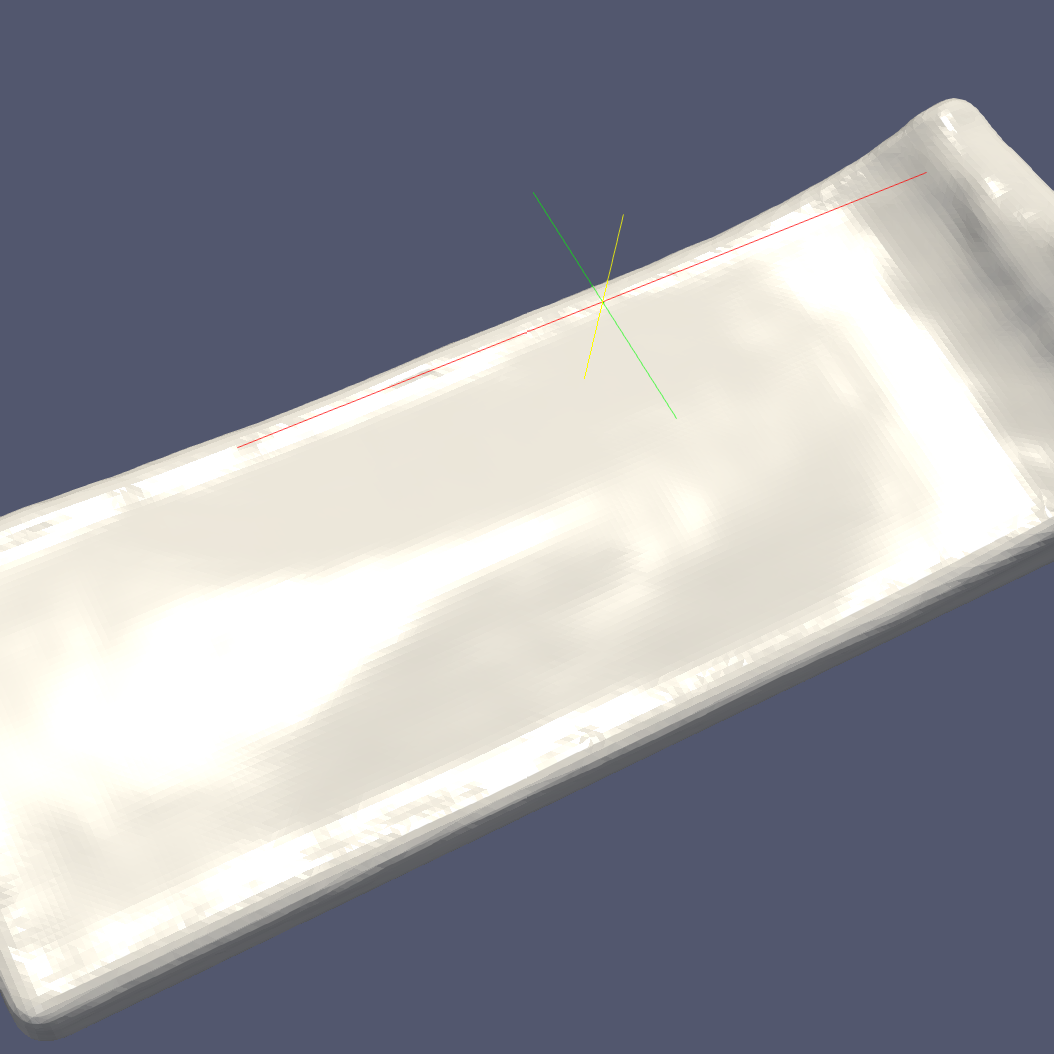
\includegraphics[width=\textwidth]{figures/Mls2Surface5Iteration.png}
			\caption{Mls correction 5 iterations}
		\end{subfigure}
	\end{center}
	\caption{Reconstructed mls surface} 
	\label{fig:mls_surf_iter_examples2}
\end{figure}

The more iterations are applied for the mls correction the smoother surface we receive. However, the most of the smoothing work is done during first two or three iterations. Sum of squared errors falls very fast during first two iterations and stays on the same level during further iteration, which means that there is not much smoothing applied to the level set after the first two iterations. On the other hand according to the figure \ref{fig:mls_surf_iter_examples} large amount of iteration can destroy tiny fluid features, such as splashes and thin areas near the border of the fluid surface. This can be controlled via calibration of the smoothing factor, but for the purpose of this thesis, removal of small frequency bumps on the reconstructed surface, one iteration is enough in most cases.

\section{Performance analysis}
The performance of the mls smoothing filter will be measured w.r.t. the number of MlsSamples, MaxMlsSamples, number of iterations. All measurements was performed on the AMD Ryzen 5 3550H. For transparent algorithm evaluation all computations were performed on single processor. All evaluations are displayed in seconds. Reconstruction was performed on the 2 frames of fluid scene with 40000 SPH particles. Note that in the mls reconstructions $updateLevelSet$ is a total of underlying methods initial $updateLevelSet$ and $mlsSmoothPath$ applied on top of that.\\
Table \ref{tab:mls_initial_method} shows the evaluated performance density based reconstruction method.
\begin{table}[H]
	\begin{center}
		\scriptsize
		\begin{tabular}{|l|c|}
			\hline
			Stage & time \\
			\hline
				configureHashTables	&	0.076903\\
				getTriangles	&	0.499455\\
				total execution time	&	6.029499\\
				updateGrid	&	1.337325\\
				updateLevelSet	&	3.736989\\
				updateSurfaceParticles	&	0.287444\\
			\hline
		\end{tabular}
	\end{center}
	\caption{Initial performance evaluation for density based reconstruction}
	\label{tab:mls_initial_method}
\end{table}
Table \ref{tab:mls_ms_perf} shows evaluated performance of the mls filter depending on the number of samples taken for the computation of mls surface (MlsSamples). In this test MlsMaxSamples is explicitly set to the MlsSamples
\begin{table}[H]
	\begin{center}
		\scriptsize
		\begin{tabular}{|l|c|c|c|}
			\hline
			MlsSamples & 100 & 200 & 300 \\
			\hline
			configureHashTables		&	0.078537	&	0.076541	&	0.083138\\
			getTriangles			&	0.538212	&	0.510159	&	0.505589\\
			mlsSmoothPath			&	33.357061	&	72.295714	&	119.967774\\
			total execution time	&	39.713907	&	78.652220	&	126.201645\\
			updateGrid				&	1.459942	&	1.461316	&	1.437795\\
			updateLevelSet			&	37.277470	&	76.245051	&	123.824661\\
			updateSurfaceParticles	&	0.289628	&	0.287632	&	0.286882\\
			\hline
		\end{tabular}
	\end{center}
	\caption{Initial performance evaluation for density based reconstruction}
	\label{tab:mls_ms_perf}
\end{table}
Table \ref{tab:mls_mms_perf} shows evaluated performance of the mls filter depending on the number of maximum number of samples  (MaxMlsSamples) taking fixed number of MlsSamples, in this test MlsSamples=400.
\begin{table}[H]
	\begin{center}
		\scriptsize
		\begin{tabular}{|l|c|c|c|c|}
			\hline
			MaxMlsSamples & 50 & 100 & 150 & 200 \\
			\hline
			configureHashTables     	& 0.081193	&	0.081389	& 0.078795		& 0.077161\\
			getTriangles    			& 0.566251	&	0.565616	& 0.554958		& 0.535509\\
			mlsSmoothPath   			& 87.600709	&	94.290563	& 104.010487	& 116.572329\\
			total execution time    	& 94.378367	&	100.942730	& 110.744296	& 123.356513\\
			updateGrid      			& 1.585025	&	1.531106	& 1.586204		& 1.596259\\
			updateLevelSet  			& 91.765409	&	98.396836	& 108.144850	& 120.773621\\
			updateSurfaceParticles  	& 0.301292	&	0.298913	& 0.307338		& 0.308659\\
			\hline
		\end{tabular}
	\end{center}
	\caption{Initial performance evaluation for density based reconstruction}
	\label{tab:mls_mms_perf}
\end{table}
Table \ref{tab:mls_iter_perf} shows evaluated performance of the mls filter depending on the number of filter iterations taking fixed number of MlsSamples=200, and MaxSamples=50.
\begin{table}[H]
	\begin{center}
		\scriptsize
		\begin{tabular}{|l|c|c|c|c|}
			\hline
			Iterations & 1 & 2 & 3 & 4 \\
			\hline
			configureHashTables     	& 0.076567	&	0.084189	& 0.078997		& 0.083295\\
			getTriangles    			& 0.606721	&	0.583862	& 0.644775		& 0.524303\\
			mlsSmoothPath   			& 49.395048	&	97.056469	& 144.075857	& 187.602832\\
			total execution time    	& 56.223171	&	103.919529	& 151.014921	& 194.276611\\
			updateGrid      			& 1.578684	&	1.586247	& 1.566563		& 1.565801\\
			updateLevelSet  			& 53.585239	&	101.285508	& 148.343585	& 191.733618\\
			updateSurfaceParticles  	& 0.301436	&	0.311386	& 0.300734		& 0.304806\\
			\hline
		\end{tabular}
	\end{center}
	\caption{Performance evaluation depending on the number of smoothing iterations}
	\label{tab:mls_iter_perf}
\end{table}

Table \ref{tab:cluster_factor} shows evaluated performance of the mls filter depending on the ClusterFactor.
\begin{table}[H]
	\begin{center}
		\scriptsize
		\begin{tabular}{|l|c|c|c|c|c|}
			\hline
			ClusterFactor & 0.1 & 0.2 & 0.4 & 0.8 & 1 \\
			\hline
			configureHashTables    	&	0.076390	&	0.074464	&	0.076946	&	0.078014	&	0.077265\\
			getTriangles    		&	0.501665	&	0.503932	&	0.504590	&	0.510349	&	0.507719\\
			mlsSmoothPath   		&	4.791562	&	8.289250	&	15.761765	&	29.372052	&	36.577372\\
			total execution time   	&	13.610064	&	17.358378	&	24.563267	&	38.239182	&	45.699859\\
			updateGrid      		&	1.448008	&	1.456376	&	1.434868	&	1.465417	&	1.458499\\
			updateLevelSet  		&	11.196505	&	14.933524	&	22.164599	&	35.807620	&	43.258932\\
			updateSurfaceParticles 	&	0.291530	&	0.291450	&	0.290358	&	0.290106	&	0.293439\\
			\hline
		\end{tabular}
	\end{center}
	\caption{Performance evaluation depending on the size of the ClusterFactor}
	\label{tab:cluster_factor}
\end{table}

In general all parameters shows linear time expansion on the reconstruction time for $mlsSmoothPath$ stage.

\section{Surface reconstruction results}
In this section some scenes representing the quality of the filter and reconstructed surface are shown. 
Figure \ref{fig:db_mls_reconstruction1} and \ref{fig:db_mls_reconstruction2} shows the reconstructed surface using density based method.
\begin{figure}
	\begin{center}
		\begin{subfigure}[b]{0.47\textwidth}
			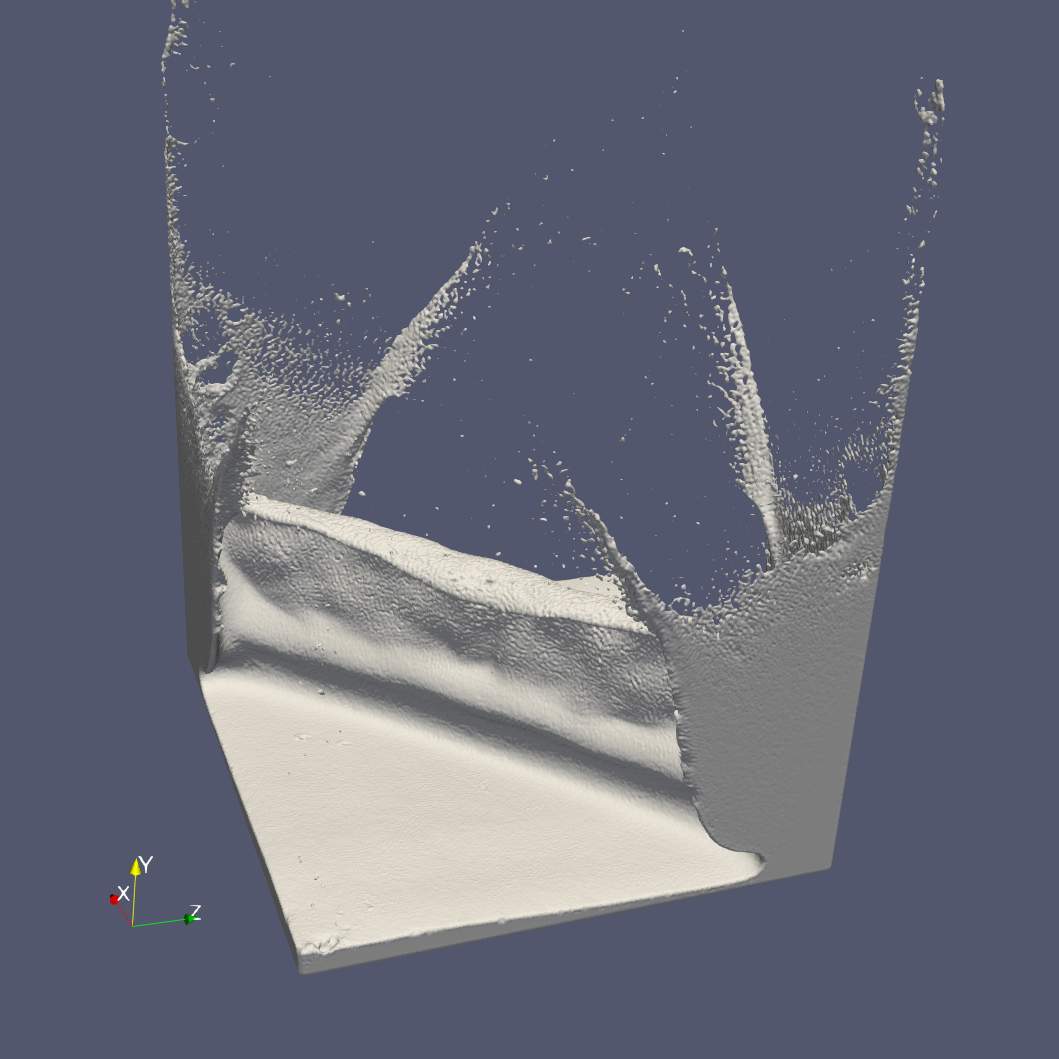
\includegraphics[width=\textwidth]{figures/DDMOriginal1.png}
			\caption{original surface}
		\end{subfigure}
		\begin{subfigure}[b]{0.47\textwidth}
			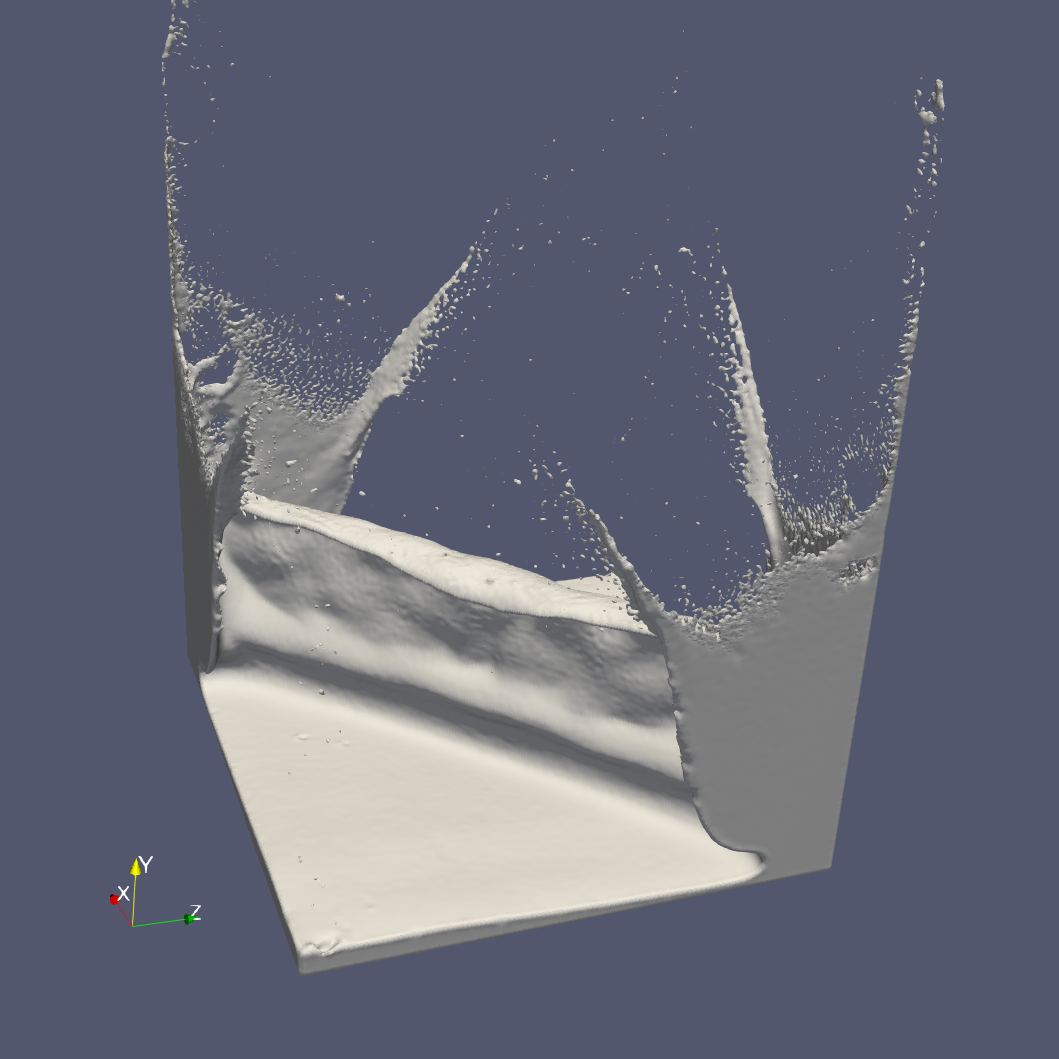
\includegraphics[width=\textwidth]{figures/DDMMls1.png}
			\caption{Mls correction smoothed}
		\end{subfigure}
		\begin{subfigure}[b]{0.47\textwidth}
			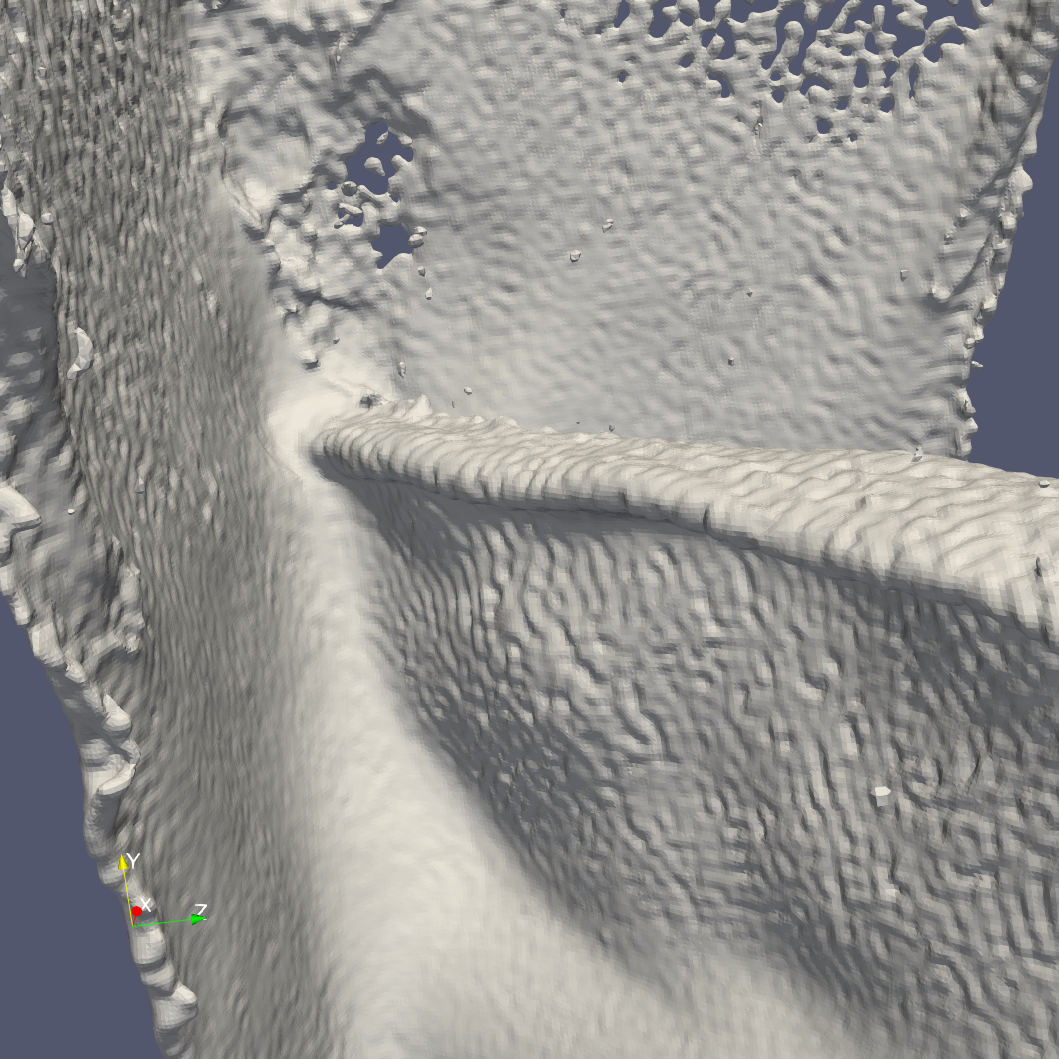
\includegraphics[width=\textwidth]{figures/DDMOriginal2.png}
			\caption{original surface}
		\end{subfigure}
		\begin{subfigure}[b]{0.47\textwidth}
			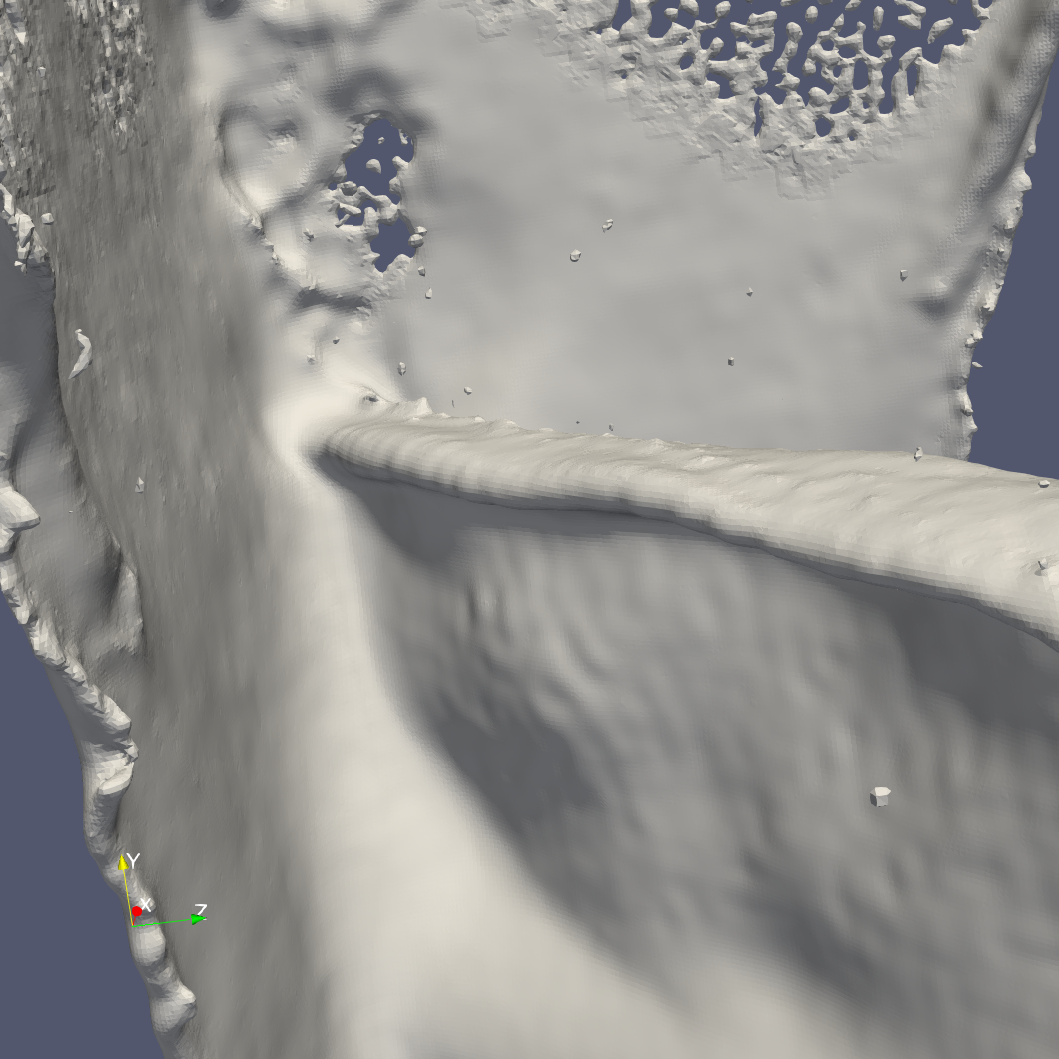
\includegraphics[width=\textwidth]{figures/DDMMls2.png}
			\caption{Mls correction smoothed}
		\end{subfigure}
	\end{center}
	\caption{Original density based surface with mls smoothing comparison} \label{fig:db_mls_reconstruction1}
\end{figure}
\begin{figure}
	\begin{center}
		\begin{subfigure}[b]{0.47\textwidth}
			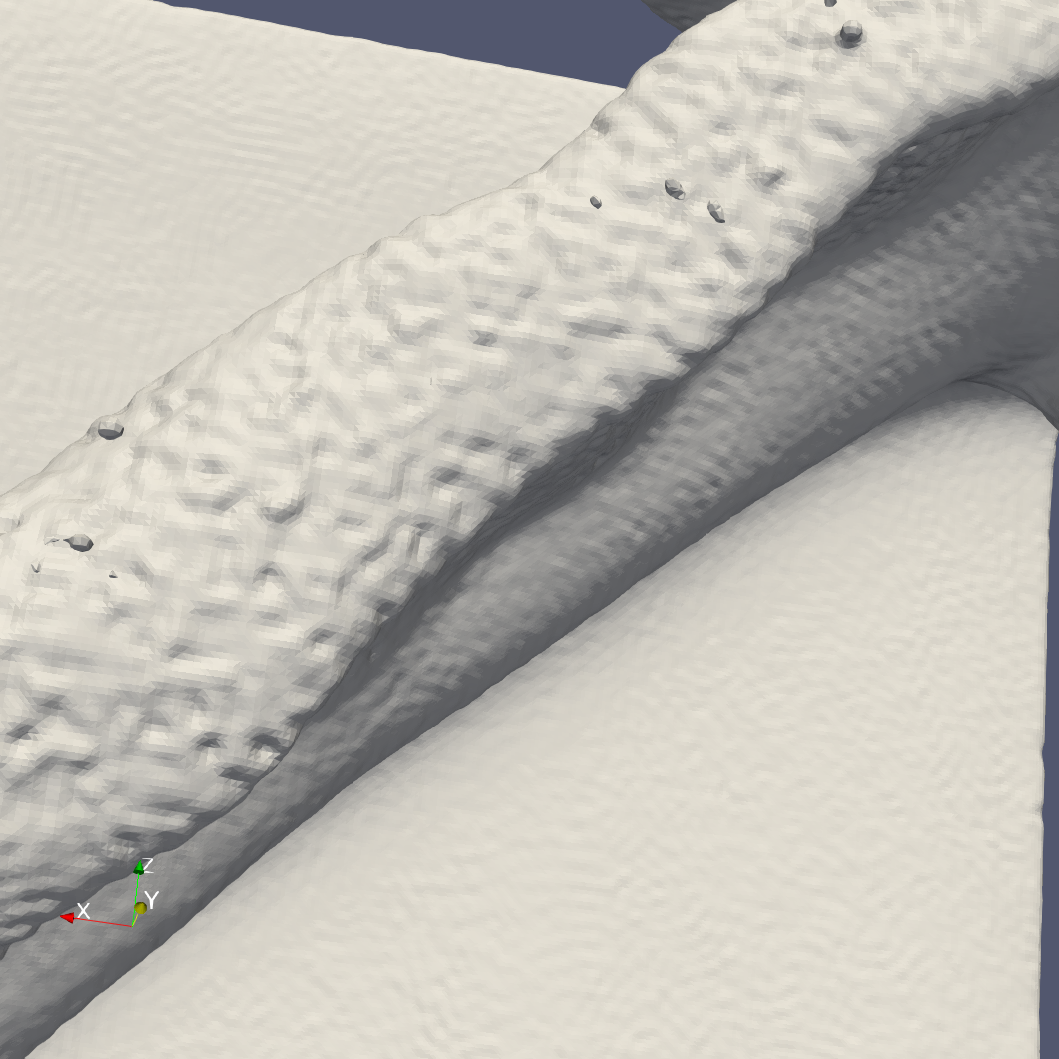
\includegraphics[width=\textwidth]{figures/DDMOriginal3.png}
			\caption{original surface}
		\end{subfigure}
		\begin{subfigure}[b]{0.47\textwidth}
			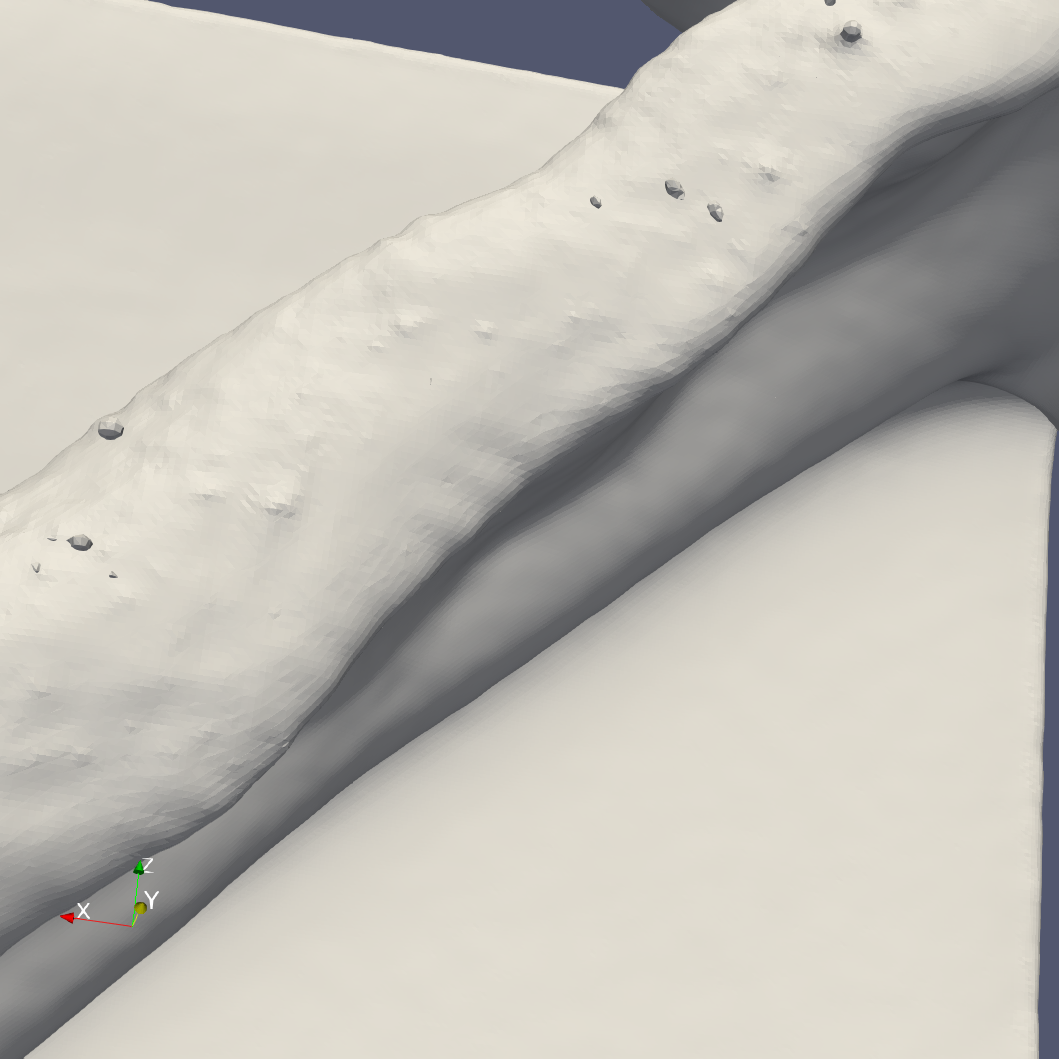
\includegraphics[width=\textwidth]{figures/DDMMls3.png}
			\caption{Mls correction smoothed}
		\end{subfigure}
		\begin{subfigure}[b]{0.47\textwidth}
			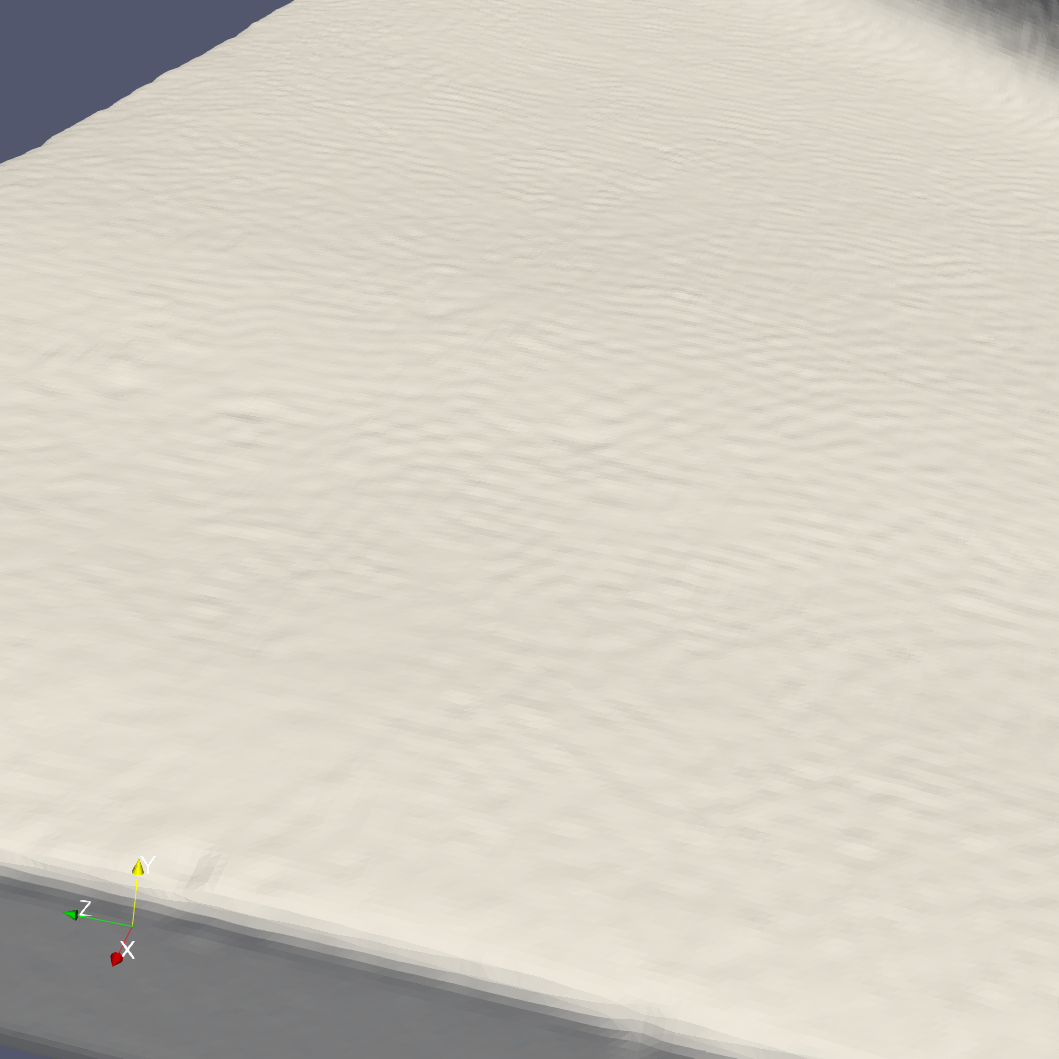
\includegraphics[width=\textwidth]{figures/DDMOriginal4.png}
			\caption{original surface}
		\end{subfigure}\begin{subfigure}[b]{0.47\textwidth}
			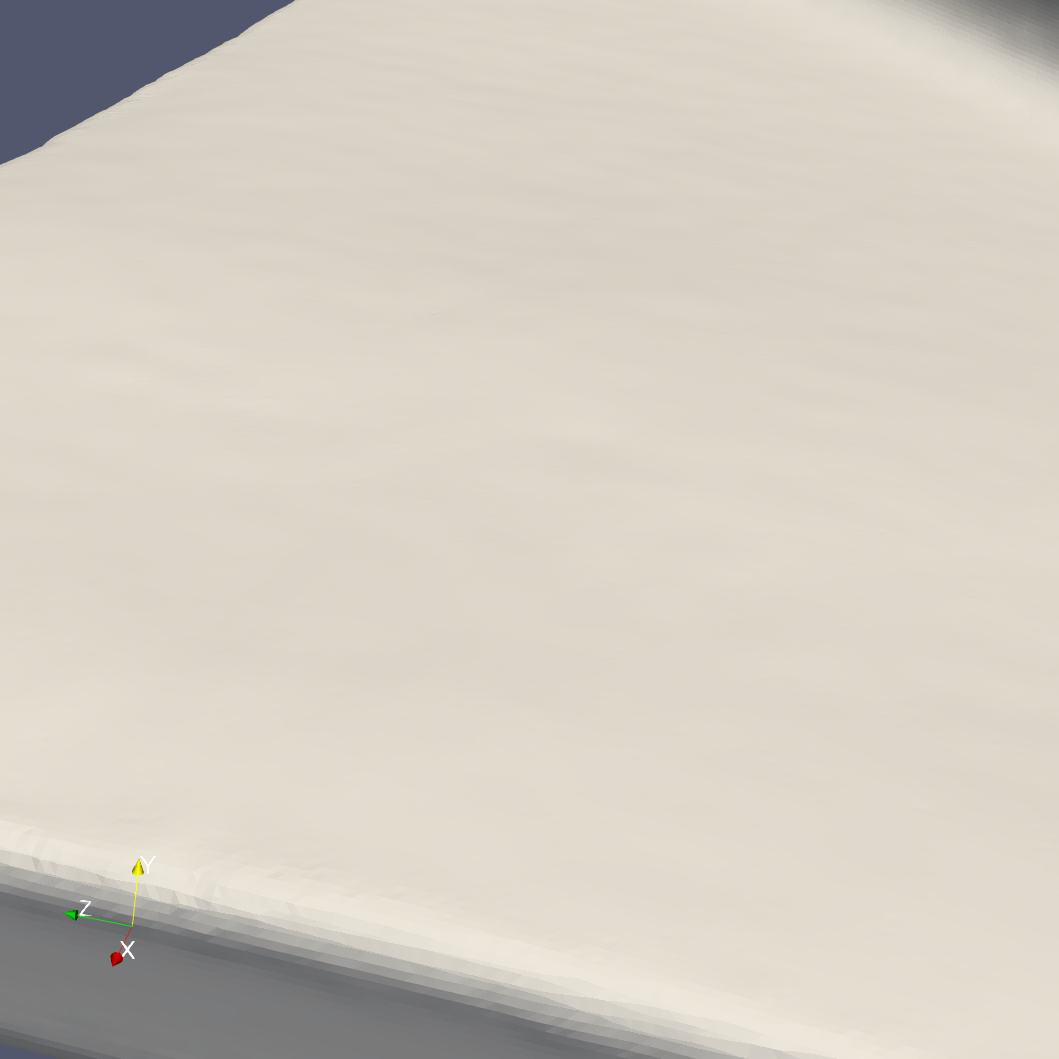
\includegraphics[width=\textwidth]{figures/DDMMls4.png}
			\caption{Mls correction smoothed}
		\end{subfigure}
	\end{center}
	\caption{Original density based surface with mls smoothed surface comparison} \label{fig:db_mls_reconstruction2}
\end{figure}
On Figures \ref{fig:db_mls_reconstruction3} and \ref{fig:db_mls_reconstruction4} surface reconstruction of canyon scene is presented.

\begin{figure}
	\begin{center}
		\begin{subfigure}[b]{0.47\textwidth}
			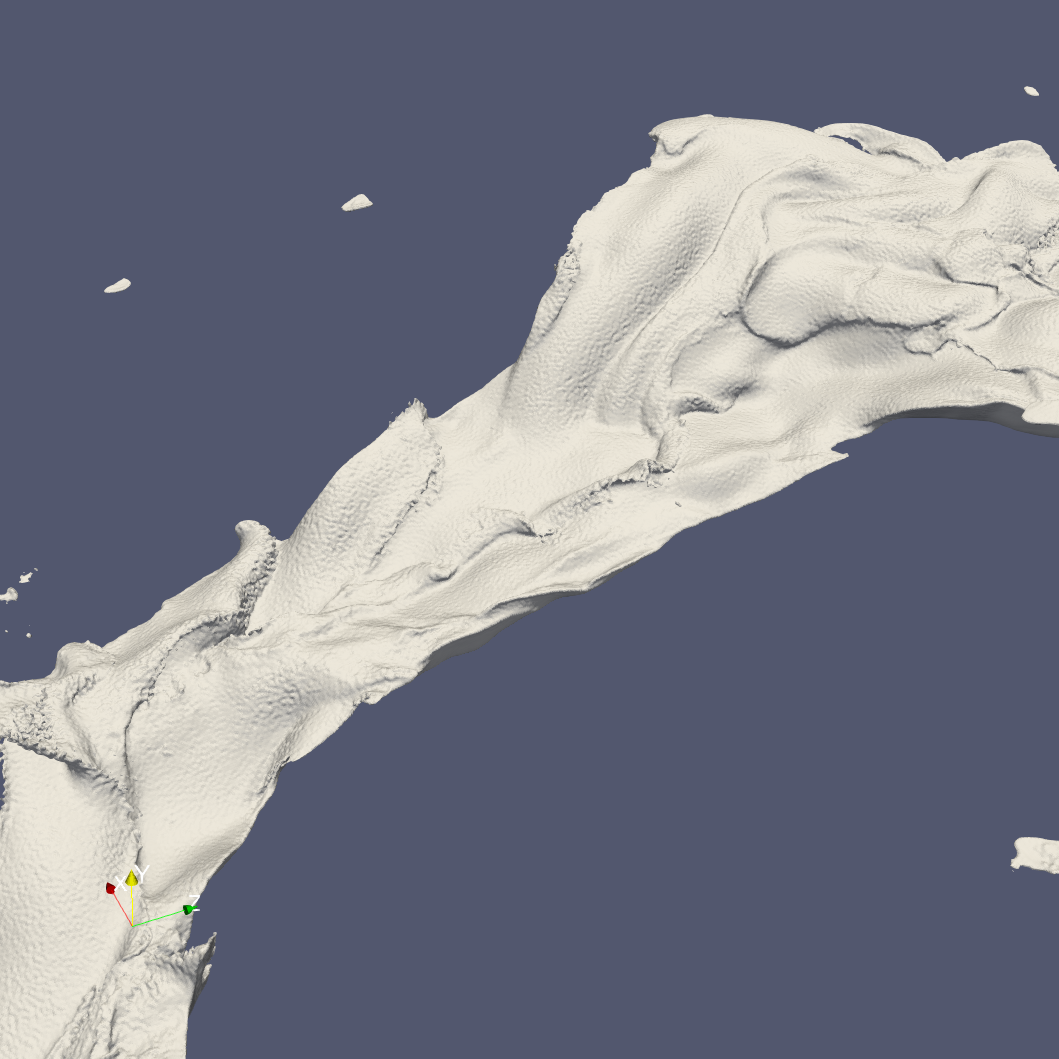
\includegraphics[width=\textwidth]{figures/CanionOriginal1.png}
			\caption{original surface}
		\end{subfigure}
		\begin{subfigure}[b]{0.47\textwidth}
			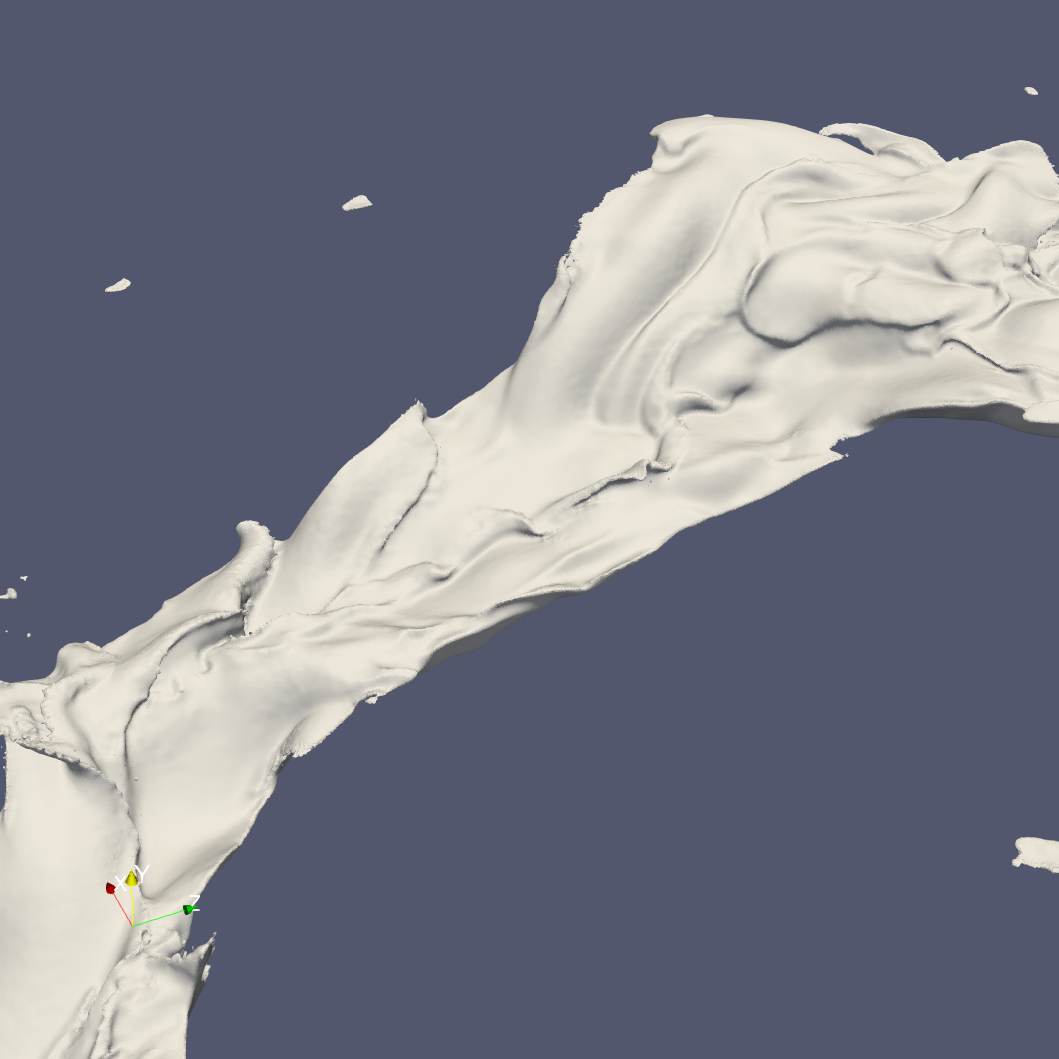
\includegraphics[width=\textwidth]{figures/CanionMls1.png}
			\caption{Mls correction smoothed}
		\end{subfigure}
		\begin{subfigure}[b]{0.47\textwidth}
			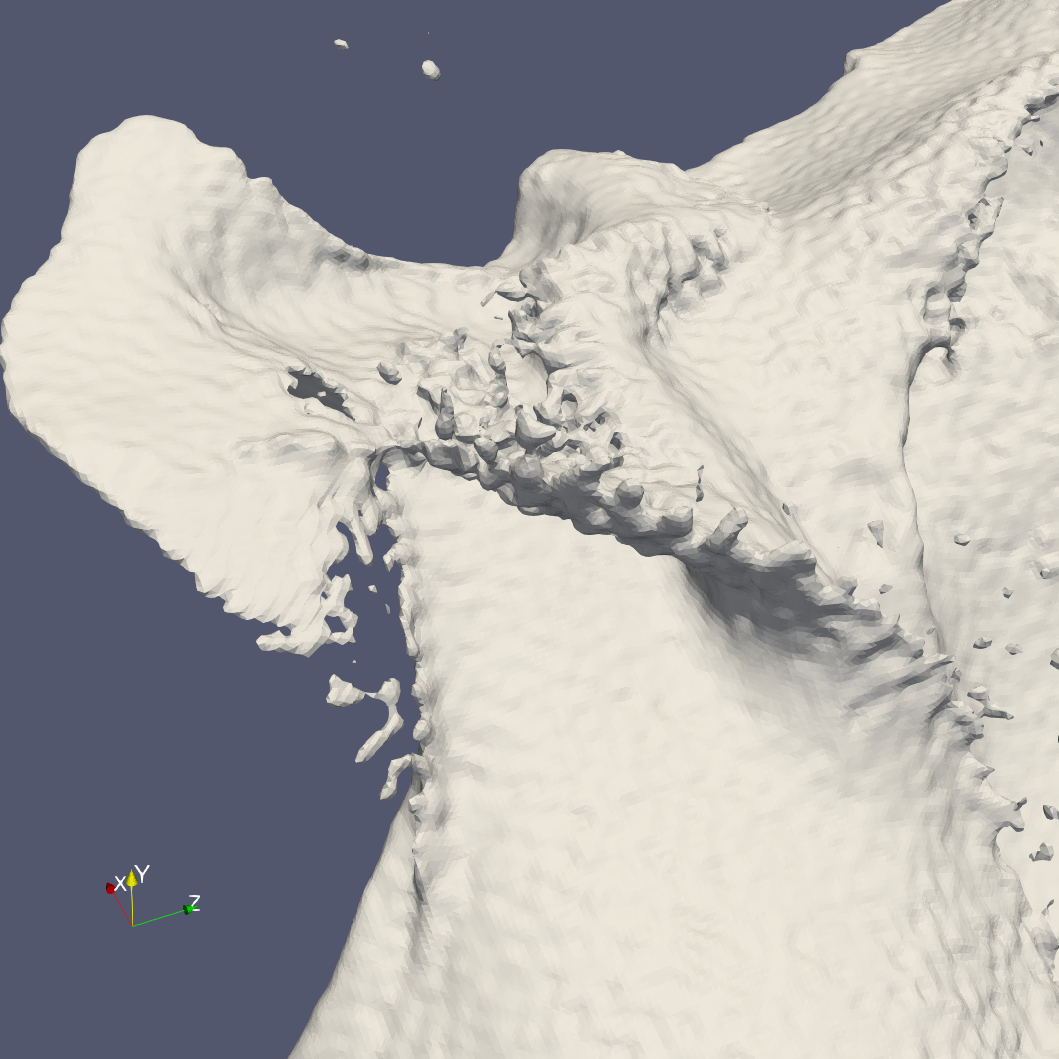
\includegraphics[width=\textwidth]{figures/CanionOriginal2.png}
			\caption{original surface}
		\end{subfigure}
		\begin{subfigure}[b]{0.47\textwidth}
			\includegraphics[width=\textwidth]{figures/CanionMls2.png}
			\caption{Mls correction smoothed}
		\end{subfigure}
	\end{center}
	\caption{Original density based surface with mls smoothing comparison} \label{fig:db_mls_reconstruction3}
\end{figure}
\begin{figure}
	\begin{center}
		\begin{subfigure}[b]{0.47\textwidth}
			\includegraphics[width=\textwidth]{figures/CanionOriginal3.png}
			\caption{Mls correction smoothed}
		\end{subfigure}
		\begin{subfigure}[b]{0.47\textwidth}
			\includegraphics[width=\textwidth]{figures/CanionMls3.png}
			\caption{original surface}
		\end{subfigure}
		\begin{subfigure}[b]{0.47\textwidth}
			\includegraphics[width=\textwidth]{figures/CanionOriginal4.png}
			\caption{Mls correction smoothed}
		\end{subfigure}
		\begin{subfigure}[b]{0.47\textwidth}
			\includegraphics[width=\textwidth]{figures/CanionMls4.png}
			\caption{original surface}
		\end{subfigure}
	\end{center}
	\caption{Original density based surface with mls smoothing comparison} \label{fig:db_mls_reconstruction4}
\end{figure}
\section{Conclusion and Future Work}
Mls smoothing filter proven to be a good alternative of blur filter. The mls filter is is much more stable then the blur filter. As was already shown iterative application of the method converges to some defined surface. Iterative application doesn't destroys continuous areas of the surface. The filter could be configured so, that small features, such that droplets or splashes in the reconstructed scene could be preserved, in the mean time undesired bumps are removed.\\
However, the most negative disadvantage of applying the mls filter is its computation time. The total complexity of the algorithm  is $O(n*m)$, where $n$ is set of 0-level intersection cells and $m$ is a set of MlsSamples. By applying Monte Carlo approaches it is possible to uniformly sample $N \subseteq n$ and $M \subseteq m$, such that the total execution time of the reconstruction could be decreased, not sacrificing too much the final quality of the reconstructed surface.\\
The future work can be applied to massively parallelize the algorithm so that it can be ran on the HPC clusters, or even port the computations on the GPU. In this work OpenMP injections was applied to parallelize all stages of the smoothing algorithms as well as reconstruction algorithms. However, current implementation contains a lot of data dependences, which is unsuitable for massively parallel architectures like resent GPGPU's.\\ Another way the algorithm can be used is generation of dataset, which can be used as a training set for a deep multi-output regression neural network analogically to \cite{DNNNoiseFilter}.